\documentclass[11pt,oneside,openany]{book}
\usepackage[paper=a4paper,top=2.2cm,bottom=2.2cm,left=2.5cm,right=2.2cm]{geometry}
\usepackage[T1]{fontenc}
\usepackage[utf8]{inputenc}
\usepackage{lmodern}
\usepackage{amsmath,amssymb,mathtools,bm}
\usepackage{graphicx}
\usepackage{booktabs,tabularx,longtable,array,multirow}
\usepackage{enumitem}
\usepackage{listings}
\usepackage{microtype}
\usepackage{caption,subcaption}
\usepackage{hyperref}
\usepackage{cleveref}

\hypersetup{hidelinks,pdftitle={Simulim dhe Metoda Numerike},pdfauthor={Klaudio Peqini}}
\graphicspath{{figures/}}
\setlength{\parindent}{1.25em}
\setlength{\parskip}{0pt}
\setlist{itemsep=.1em,topsep=.2em,parsep=0pt}
\captionsetup{font=small,labelfont=bf}
\pagestyle{plain}
\newcolumntype{Y}{>{\raggedright\arraybackslash}X}
\newcommand{\vect}[1]{\bm{#1}}
\newcommand{\E}{\mathbb{E}}
\newcommand{\Var}{\operatorname{Var}}
\newcommand{\Cov}{\operatorname{Cov}}
\newcommand{\R}{\mathbb{R}}
\newcommand{\dd}{\,\mathrm{d}}
\newcommand{\Oh}{\mathcal{O}}
\newcommand{\avg}[1]{\left\langle #1\right\rangle}
\renewcommand{\contentsname}{Përmbajtja}
\renewcommand{\chaptername}{Kapitulli}
\renewcommand{\figurename}{Figura}
\renewcommand{\tablename}{Tabela}
\renewcommand{\bibname}{Literatura}
\setcounter{tocdepth}{1}
\makeatletter
\renewcommand*\l@section{\@dottedtocline{1}{1.5em}{3.2em}}
\makeatother
\newenvironment{qellime}{\par\medskip\noindent\textbf{Rezultatet e të nxënit.}\ }{\par\medskip}
\newenvironment{shembull}[1][]{\par\medskip\noindent\textbf{Shembull #1.}\ }{\par\medskip}
\newenvironment{kujdes}{\par\medskip\noindent\textbf{Kujdes numerik.}\ }{\par\medskip}
\newenvironment{lidhje}{\par\medskip\noindent\textbf{Lidhja me laboratorin.}\ }{\par\medskip}
\lstdefinestyle{scientific}{basicstyle=\ttfamily\footnotesize,keywordstyle=\bfseries,commentstyle=\itshape,showstringspaces=false,frame=single,framerule=.3pt,breaklines=true,columns=fullflexible,literate={ë}{{\"e}}1 {Ë}{{\"E}}1 {ç}{{\c c}}1 {Ç}{{\c C}}1}
\lstset{style=scientific}

\begin{document}
\frontmatter
\begin{titlepage}
\centering
\vspace*{1.5cm}
{\Large Universiteti i Tiranës\\Fakulteti i Shkencave të Natyrës\\Departamenti i Fizikës\par}
\vspace{2.2cm}
{\Huge\bfseries Simulim dhe Metoda Numerike\par}
\vspace{.6cm}
{\LARGE Leksione të shkruara\par}
\vspace{1.4cm}
{\Large Bachelor në Fizikë dhe Shkenca Kompjuterike\par}
\vfill
{\large Prof. Asoc. Dr. Klaudio Peqini\par}
\vspace{.4cm}
{\large Viti akademik 2026--2027\par}
\end{titlepage}

\chapter*{Parathënie}
Ky tekst përmbledh në një tërësi koherente përmbajtjen e lëndës \emph{Simulim dhe Metoda Numerike}, me 30 orë leksione dhe 30 orë laborator. Ai vazhdon filozofinë e kursit \emph{Modelim në Fizikë}: nga pyetja fizike te modeli matematik, nga modeli te algoritmi dhe nga algoritmi te një eksperiment numerik i verifikueshëm e i riprodhueshëm. Theksi i ri vendoset te gabimi numerik, kampionimi, simulimi stokastik dhe metodat Monte Carlo.

Teksti nuk e lidh metodën shkencore me një gjuhë të vetme programimi. Shembujt mund të realizohen në Python ose MATLAB/Octave. Notebook-u përdoret për të bashkuar shpjegimin, kodin, figurat dhe interpretimin; funksionet dhe paketat përdoren për kod të ripërdorshëm. Termat \emph{bredhje}, \emph{statistike} dhe \emph{pacaktueshmëri} përdoren në mënyrë të njëtrajtshme në të gjithë tekstin.

\begin{figure}[h]
\centering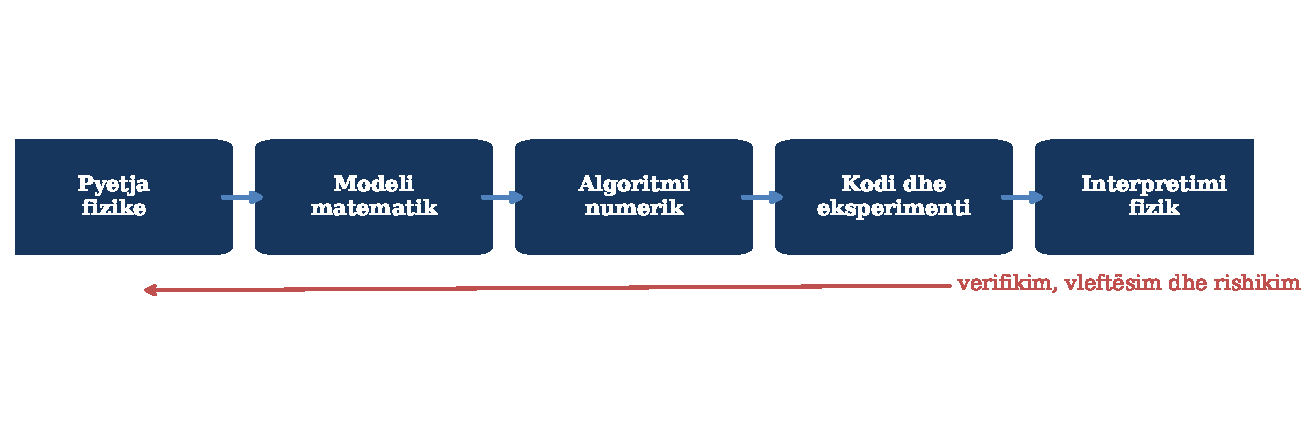
\includegraphics[width=.96\textwidth]{01_cikli_simulimit.pdf}
\caption{Cikli i punës në simulimin fizik. Rezultati kthehet te pyetja fillestare përmes verifikimit dhe vleftësimit.}
\end{figure}

\chapter*{Si të përdoret ky tekst}
Çdo kapitull përmban objektiva, teori, shembuj fizikë, algoritme, analiza të gabimit, lidhje me laboratorin dhe pyetje kontrolli. Leximi duhet të shoqërohet me ekzekutimin e notebook-ut përkatës. Kur paraqitet një rezultat numerik, studenti duhet të jetë në gjendje të përgjigjet: cilin model po zgjidhim, me cilën metodë, me çfarë gabimi dhe me cilat kufizime fizike?

\tableofcontents
\mainmatter
\chapter{Hyrje në simulimet fizike dhe programimin shkencor}
\begin{qellime}
Studenti dallon sistemin real, modelin matematik, algoritmin dhe kodin; formulon hyrjet, daljet dhe supozimet; dallon simulimin determinist nga ai stokastik; organizon një eksperiment të riprodhueshëm në Python ose MATLAB/Octave.
\end{qellime}

\section{Nga modeli te eksperimenti numerik}
Një simulim fizik është një eksperiment i kryer mbi një model. Ai nuk fillon me kodin, por me një pyetje: cilën madhësi kërkojmë, në çfarë kushtesh dhe me çfarë saktësie? Sistemi real përmban më shumë hollësi sesa mund të përfaqësohen. Modelimi zgjedh mekanizmat dominues, ndërsa simulimi zbaton pasojat e kësaj zgjedhjeje.

Një problem dinamik mund të shkruhet në formën
\begin{equation}
 \frac{\dd \vect y}{\dd t}=\vect f(t,\vect y;\vect\theta),\qquad \vect y(t_0)=\vect y_0,
\end{equation}
ku $\vect y$ është gjendja dhe $\vect\theta$ përmbledh parametrat. Për një grimcë në një përmasë, $\vect y=(x,v)^T$. Në një model stokastik, evolucioni varet edhe nga një ndryshore rasti $\xi_n$,
\begin{equation}
 \vect Y_{n+1}=\vect G(t_n,\vect Y_n;\vect\theta,\xi_n).
\end{equation}
Një ekzekutim determinist jep të njëjtën trajektore për të njëjtat hyrje; një ekzekutim stokastik jep një realizim. Përfundimi stokastik merret nga bashkësia e realizimeve.

\section{Hierarkia e modeleve}
Modelet ndërtohen në nivele. Modeli minimal izolon mekanizmin kryesor dhe lehtëson kontrollin analitik. Modeli i zgjeruar shton fërkim, forcë të jashtme, zhurmë ose gjeometri reale. Modeli më kompleks nuk është domosdoshmërisht më i mirë: ai kërkon më shumë parametra, të dhëna dhe prova vleftësimi.

\begin{shembull}[Rënia e lirë]
Pa rezistencë ajri, $y(t)=y_0+v_0t-gt^2/2$. Ky rast ka zgjidhje analitike dhe përdoret për verifikim. Me rezistencë lineare, $m\dot v=-mg-cv$; me rezistencë kuadratike, $m\dot v=-mg-cv|v|$. Zgjedhja ndërmjet tyre është vendim fizik, jo programues.
\end{shembull}

\section{Diskretizimi}
Kompjuteri ruan një numër të fundmë vlerash. Koha zëvendësohet nga rrjeti
\begin{equation}
 t_n=t_0+n\Delta t,\qquad n=0,1,\ldots,N.
\end{equation}
Hapi $\Delta t$ kontrollon rezolucionin dhe koston. Një hap më i vogël zakonisht ul gabimin e këputjes, por rrit numrin e veprimeve dhe mund të ekspozojë gabimin e rrumbullakimit. Përzgjedhja e hapit duhet të mbështetet në një studim konvergjence.

\section{Programimi shkencor}
Programimi shkencor e kthen arsyetimin në një procedurë që mund të përsëritet. Një notebook i mirë përmban: pyetjen fizike; supozimet; parametrat dhe njësitë; funksionet; eksperimentet; figurat; analizën e gabimit; përfundimin. Parametrat nuk duhen fshehur brenda funksioneve. Një funksion duhet të kryejë një detyrë të qartë dhe të kthejë rezultate që mund të testohen.

\begin{table}[ht]
\centering
\caption{Dy rrugë teknike me të njëjtin standard shkencor.}
\begin{tabularx}{\textwidth}{YY}
\toprule Python & MATLAB/Octave\\ \midrule
NumPy për vektorë dhe matrica & Vektorë dhe matrica si objekte bazë\\
Matplotlib për figura & \texttt{plot} dhe funksionet grafike\\
Funksione dhe module \texttt{.py} & Funksione dhe skripte \texttt{.m}\\
Jupyter Notebook & Jupyter me kernel Octave ose Live Script\\
\bottomrule
\end{tabularx}
\end{table}

\section{Verifikimi, vleftësimi dhe riprodhueshmëria}
Verifikimi pyet nëse kodi zgjidh saktë ekuacionet e zgjedhura. Vleftësimi pyet nëse ekuacionet përshkruajnë mjaftueshëm sistemin real për qëllimin e deklaruar. Verifikimi përdor zgjidhje analitike, ligje ruajtjeje, teste njësish dhe konvergjencë. Vleftësimi përdor matje, parametra të kalibruar dhe krahasim me modele alternative.

Riprodhueshmëria kërkon kodin, të dhënat, versionet e paketave, parametrat, farën e gjeneratorit dhe rendin e ekzekutimit. Një figurë pa këto të dhëna është dëshmi e paplotë.

\begin{lidhje}
Laboratori 1 ndërton të njëjtin notebook në njërën prej dy gjuhëve. Versioni i instruktorit shërben për shpjegim; versioni i studentit duhet të përmbajë arsyetimin, kodin dhe interpretimin e vet.
\end{lidhje}

\section*{Pyetje kontrolli}
\begin{enumerate}
\item Jepni një shembull ku kodi është i saktë, por modeli fizik është i papërshtatshëm.
\item Pse zvogëlimi i hapit nuk garanton gjithmonë përmirësim?
\item Cilat të dhëna duhen ruajtur për një eksperiment Monte Carlo të riprodhueshëm?
\end{enumerate}
\section{Algoritmi bazë i një eksperimenti numerik}
Algoritmi kryesor i kapitullit nuk është një formulë e vetme, por cikli i plotë i punës. Ai duhet të përdoret në çdo notebook të kursit.

\begin{enumerate}
\item Formulohet pyetja fizike dhe përcaktohet madhësia e daljes.
\item Shënohen supozimet, njësitë, parametrat dhe kushtet fillestare.
\item Zgjidhet modeli minimal që mund t'i përgjigjet pyetjes.
\item Përcaktohen rrjeti, algoritmi, toleranca dhe kriteri i ndalimit.
\item Shkruhet kodi si funksione të testueshme.
\item Verifikohet me një rast analitik ose një ligj ruajtjeje.
\item Kryhet studimi i konvergjencës ose i numrit të mostrave.
\item Raportohen rezultati, gabimi numerik, pacaktueshmëria dhe kufijtë e modelit.
\end{enumerate}

\subsection{Një skelet Python për notebook-un}
\begin{lstlisting}[language=Python,caption={Skelet minimal për një eksperiment numerik.}]
from dataclasses import dataclass
import numpy as np
import matplotlib.pyplot as plt

@dataclass(frozen=True)
class Parametra:
    y0: float = 1.5       # m
    v0: float = 8.0       # m/s
    g: float = 9.81       # m/s^2
    t_fund: float = 1.2   # s
    dt: float = 0.02      # s

def modeli_analitik(t, p):
    """Pozicioni vertikal pa rezistence ajri."""
    return p.y0 + p.v0*t - 0.5*p.g*t**2

def eksperiment(p):
    t = np.arange(0.0, p.t_fund + p.dt/2, p.dt)
    y = modeli_analitik(t, p)
    assert np.isclose(y[0], p.y0)
    return t, y

p = Parametra()
t, y = eksperiment(p)
plt.plot(t, y)
plt.xlabel("Koha t [s]")
plt.ylabel("Lartesia y [m]")
plt.grid(alpha=0.25)
plt.show()
\end{lstlisting}

\subsection{Kontrolli i riprodhueshmërisë}
Për simulime stokastike përdoret një gjenerator i deklaruar, jo gjendja globale e fshehur.
\begin{lstlisting}[language=Python]
rng = np.random.default_rng(2026)
mostra = rng.normal(loc=0.0, scale=1.0, size=10_000)
\end{lstlisting}
Fara nuk e bën rezultatin ``më të rastit''; ajo identifikon realizimin. Në raport shënohen fara, numri i mostrave dhe versionet e bibliotekave.

\subsection{Terminologji dhe stil shkencor}
Në këtë tekst përdoren \emph{zbatim} për implementation, \emph{rrjetë} për grid, \emph{hap} për step, \emph{mbetje} për residual, \emph{vleftësim} për validation dhe \emph{riprodhueshmëri} për reproducibility. Kodi nuk duhet të fshehë njësitë fizike; ato shënohen në komente, tabela dhe boshte.

\begin{lidhje}
Notebook-u i studentit duhet të nisë nga ky skelet dhe të ruajë ndarjen ndërmjet parametrave, modelit, eksperimentit dhe paraqitjes grafike.
\end{lidhje}

Për organizimin terminologjik të modelit, algoritmit dhe zbatimit numerik janë konsultuar tekstet universitare shqip të analizës numerike \cite{hanelli,hoxha,datja}, krahas literaturës ndërkombëtare të fizikës llogaritëse \cite{newman,landau}.

\subsection{Nga ligji fizik te algoritmi: një shembull i plotë}
Le të ndërtojmë modelin e rënies vertikale me rezistencë lineare të ajrit. Zgjedhim boshtin pozitiv për poshtë dhe shënojmë me $y(t)$ zhvendosjen dhe me $v(t)=\dot y(t)$ shpejtësinë. Ligji i dytë i Njutonit jep
\begin{equation}
 m\dot v=mg-cv,\qquad \dot y=v,
\end{equation}
ku $m>0$, $g>0$ dhe $c\ge0$. Përmasat fizike janë $[g]=LT^{-2}$ dhe $[c]=MT^{-1}$; prandaj $c/m$ ka përmasën e inversit të kohës. Koha karakteristike $\tau=m/c$ tregon sa shpejt humbet kujtesa e kushtit fillestar. Zgjidhja analitike,
\begin{equation}
 v(t)=v_\infty+(v_0-v_\infty)e^{-t/\tau},\qquad v_\infty=\frac{mg}{c},
\end{equation}
është një pikë reference për verifikimin e kodit. Ajo nuk përdoret sepse problemi është i vështirë, por sepse na lejon të ndajmë gabimin e algoritmit nga gabimi i modelit.

Me metodën e Eulerit, derivati në $t_n$ zëvendësohet nga diferenca përpara,
\begin{equation}
 \dot v(t_n)=\frac{v(t_n+h)-v(t_n)}{h}+\Oh(h).
\end{equation}
Duke neglizhuar termin $\Oh(h)$ dhe duke shënuar $v_n\approx v(t_n)$ merret
\begin{equation}
 v_{n+1}=v_n+h\left(g-\frac{c}{m}v_n\right),\qquad y_{n+1}=y_n+hv_n.
\end{equation}
Gabimi lokal i një hapi është $\Oh(h^2)$, ndërsa grumbullimi në një interval kohor të fiksuar jep gabim global $\Oh(h)$. Kjo dallon rendin lokal nga rendi global dhe shpjegon pse përgjysmimi i hapit duhet ta përgjysmojë afërsisht gabimin për një metodë të rendit të parë.

\begin{lstlisting}[language=Python,caption={Eksperiment konvergjence për rënien me rezistencë lineare.}]
import numpy as np

def renie_euler(m, c, g, y0, v0, T, h):
    n = int(np.ceil(T / h))
    h = T / n                 # hapi rregullohet që t_n të arrijë saktë T
    t = np.linspace(0.0, T, n + 1)
    y = np.empty(n + 1); v = np.empty(n + 1)
    y[0], v[0] = y0, v0
    for k in range(n):
        y[k + 1] = y[k] + h * v[k]
        v[k + 1] = v[k] + h * (g - (c / m) * v[k])
    return t, y, v

def v_sakte(t, m, c, g, v0):
    tau = m / c
    v_inf = m * g / c
    return v_inf + (v0 - v_inf) * np.exp(-t / tau)

for h in (0.2, 0.1, 0.05, 0.025):
    t, y, v = renie_euler(1.0, 0.4, 9.81, 0.0, 0.0, 4.0, h)
    gabimi = np.max(np.abs(v - v_sakte(t, 1.0, 0.4, 9.81, 0.0)))
    print(f"h={h:7.4f}, gabimi maksimal={gabimi:.6e}")
\end{lstlisting}
Ky program ndan modelin, integruesin dhe testin analitik. Në MATLAB/Octave të njëjtat vargje ndërtohen me \texttt{linspace} dhe cikli me \texttt{for}; ndryshimi sintaksor nuk ndryshon logjikën shkencore.

\subsection{Verifikim, vleftësim dhe analizë ndjeshmërie}
Një rezultat mund të jetë i konverguar ndaj $h\to0$ dhe përsëri të jetë fizikisht i gabuar. Konvergjenca kontrollon vetëm diskretizimin. Për vleftësim duhen të dhëna ose një model referimi. Në shembullin e mësipërm, koeficienti $c$ mund të varet nga forma, dendësia e ajrit dhe regjimi i rrjedhjes. Nëse $c$ është matur me pacaktueshmëri, kjo pacaktueshmëri duhet të përhapet deri te $v(t)$.

Ndjeshmëria lokale ndaj parametrit $c$ mund të vlerësohet me
\begin{equation}
 S_c(t)\approx\frac{v(t;c+\Delta c)-v(t;c-\Delta c)}{2\Delta c}.
\end{equation}
Vlera $S_c$ ka njësi dhe varet nga shkalla; një ndjeshmëri pa përmasa është $cS_c/v$. Në një studim të plotë raportohen veçmas gabimi i diskretizimit, pacaktueshmëria e parametrave dhe mospërputhja model--eksperiment.

\subsection{Përmbledhje dhe punë e pavarur}
Eksperimenti numerik është një zinxhir argumentesh: përkufizim i pyetjes, zgjedhje e modelit, kontroll dimensional, diskretizim, implementim, verifikim dhe interpretim fizik. Studenti duhet të jetë në gjendje të tregojë ku hyn çdo supozim dhe cilin lloj gabimi kontrollon çdo provë.

\begin{enumerate}
\item Nxirrni zgjidhjen analitike për $y(t)$ dhe përdoreni për të matur rendin e Eulerit.
\item Zëvendësoni forcën $-cv$ me $-cv|v|$ dhe përcaktoni shpejtësinë kufitare.
\item Ndërtoni të njëjtin eksperiment në MATLAB/Octave dhe krahasoni rezultatet deri në tolerancën e rrumbullakimit.
\item Shpjegoni pse krahasimi me të dhënat eksperimentale është vleftësim, ndërsa krahasimi me zgjidhjen analitike është verifikim.
\end{enumerate}

\subsection{Analiza pa përmasa dhe projektimi i simulimit}
Para se të zgjidhet një metodë numerike, është e dobishme të identifikohen shkallët karakteristike të problemit. Në modelin e rënies me rezistencë lineare,
\begin{equation}
 m\frac{\dd v}{\dd t}=mg-cv,
\end{equation}
shpejtësia karakteristike është $V=mg/c$ dhe koha karakteristike është $T=m/c$. Duke vendosur $u=v/V$ dhe $\tau=t/T$, ekuacioni bëhet
\begin{equation}
 \frac{\dd u}{\dd\tau}=1-u.
\end{equation}
Të tre parametrat dimensionalë janë reduktuar në një ekuacion universal. Kjo formë tregon se çdo trup që i bindet të njëjtit model ka të njëjtën kurbë $u(\tau)$; parametrat vetëm ndryshojnë shkallët e boshteve. Në simulim, analiza pa përmasa ndihmon në zgjedhjen e hapit: $\Delta\tau=\Delta t/T$ duhet të jetë mjaft i vogël për të përshkruar relaksimin. Ajo ndihmon edhe në testim, sepse rezultatet për grupe të ndryshme parametrash duhet të bien mbi të njëjtën kurbë të reduktuar.

Në modelin kuadratik $m\dot v=mg-cv|v|$, shpejtësia kufitare është $V=\sqrt{mg/c}$ dhe një shkallë kohe është $T=V/g$. Përsëri merret një ekuacion pa përmasa, por struktura jolineare mbetet. Krahasimi i dy modeleve duhet bërë në të njëjtat madhësi të reduktuara; përndryshe ndryshimi i njësive ose i shkallëve mund të ngatërrohet me ndryshim fizik.

\subsubsection{Nga kërkesa shkencore te kriteri i pranimit}
Një simulim duhet të fillojë me një kërkesë të matshme. Pohimi ``të simulohet lavjerrësi'' nuk përcakton as produktin, as saktësinë. Një kërkesë operative mund të jetë: ``të përcaktohet perioda për $0\le\theta_0\le1.2$ rad me gabim relativ nën $10^{-3}$ dhe të kontrollohet ruajtja e energjisë për njëqind perioda''. Kjo fjali përcakton madhësinë dalëse, domenin e parametrave, tolerancën dhe një invariant verifikimi.

Kriteri i pranimit nuk duhet të jetë vetëm ``kodi ekzekutohet''. Për një metodë të rendit $p$, raporti
\begin{equation}
 R_h=\frac{\|y_h-y_{h/2}\|}{\|y_{h/2}-y_{h/4}\|}
\end{equation}
duhet të afrohet me $2^p$ në regjimin asimptotik. Nëse kjo nuk ndodh, mund të ketë gabim implementimi, hap ende të madh, zgjidhje jo të lëmuar ose dominim të rrumbullakimit. Kriteret fizike përfshijnë shenjat, kufijtë, njësitë dhe ligjet e ruajtjes. Kriteret statistike përfshijnë përsëritjen me fara të ndryshme dhe intervalin e besimit.

\subsubsection{Hierarkia e pacaktueshmërive}
Në një raport të plotë dallohen së paku katër nivele. Pacaktueshmëria e hyrjeve vjen nga matjet e parametrave. Gabimi i modelit vjen nga mekanizmat e neglizhuar. Gabimi numerik vjen nga diskretizimi dhe aritmetika me saktësi të fundme. Gabimi i kampionimit vjen nga përdorimi i një numri të fundmë realizimesh. Zvogëlimi i hapit kontrollon vetëm një pjesë të nivelit të tretë; rritja e numrit të mostrave kontrollon vetëm nivelin e katërt. Një grafik me shumë shifra nuk mund të kompensojë një model fizik të papërshtatshëm.

Për laboratorin rekomandohet që çdo notebook të përmbajë një tabelë të shkurtër me kolonat: burimi i pacaktueshmërisë, mënyra e vlerësimit, madhësia e efektit dhe prova e kontrollit. Kjo e kthen notebook-un nga një demonstrim kodi në dokument shkencor.


\chapter{Aritmetika kompjuterike dhe analiza e gabimeve}
\begin{qellime}
Studenti përshkruan numrat me pikë të lëvizshme; dallon gabimin absolut e relativ, gabimin e përparmë e të prapmë; analizon kushtëzimin dhe qëndrueshmërinë; njeh anulimin, humbjen e rëndësisë dhe grumbullimin e gabimeve.
\end{qellime}

\section{Përfaqësimi me saktësi të fundme}
Një numër normal binar përfaqësohet si
\begin{equation}
 x=(-1)^s(1.b_1b_2\ldots b_p)_2\,2^e.
\end{equation}
Në standardin IEEE 754, formati double ka 53 bita saktësi në mantisë. Distanca relative ndërmjet numrave pranë njësisë është afërsisht $2^{-52}$. Madhësia
\begin{equation}
 u=\tfrac12\,\beta^{1-p}
\end{equation}
quhet njësia e rrumbullakimit. Modeli bazë është
\begin{equation}
 \operatorname{fl}(x\circ y)=(x\circ y)(1+\delta),\qquad |\delta|\le u,
\end{equation}
për një veprim $\circ$, me kusht që të mos ndodhë tejmbushje ose nënmbushje.

Numrat \texttt{Inf}, \texttt{-Inf} dhe \texttt{NaN} sinjalizojnë rezultate jashtë bashkësisë së numrave të fundmë ose veprime të papërcaktuara. Krahasimi i numrave realë nuk duhet të mbështetet verbërisht në barazinë bit për bit; përdoret një tolerancë që merr parasysh shkallën e problemit.

\section{Gabimi absolut dhe relativ}
Nëse $x$ është vlera e saktë dhe $\tilde x$ përafrimi,
\begin{equation}
 e_a=|\tilde x-x|,\qquad e_r=\frac{|\tilde x-x|}{|x|}.
\end{equation}
Gabimi relativ nuk ka kuptim kur $x=0$ dhe bëhet i paqëndrueshëm pranë zeros. Në vektorë përdoret një normë, për shembull
\begin{equation}
 e_r=\frac{\|\tilde{\vect x}-\vect x\|_2}{\|\vect x\|_2}.
\end{equation}

\section{Anulimi dhe humbja e shifrave}
Zbritja e dy numrave pothuaj të barabartë heq shifrat kryesore të përbashkëta dhe zmadhon gabimin relativ të mbetjes. Shprehja $\sqrt{x+1}-\sqrt{x}$ për $x\gg1$ llogaritet më mirë si
\begin{equation}
 \frac{1}{\sqrt{x+1}+\sqrt{x}}.
\end{equation}
Të dyja janë algjebrikisht të njëjta, por jo numerikisht të barasvlershme.

\begin{figure}[ht]
\centering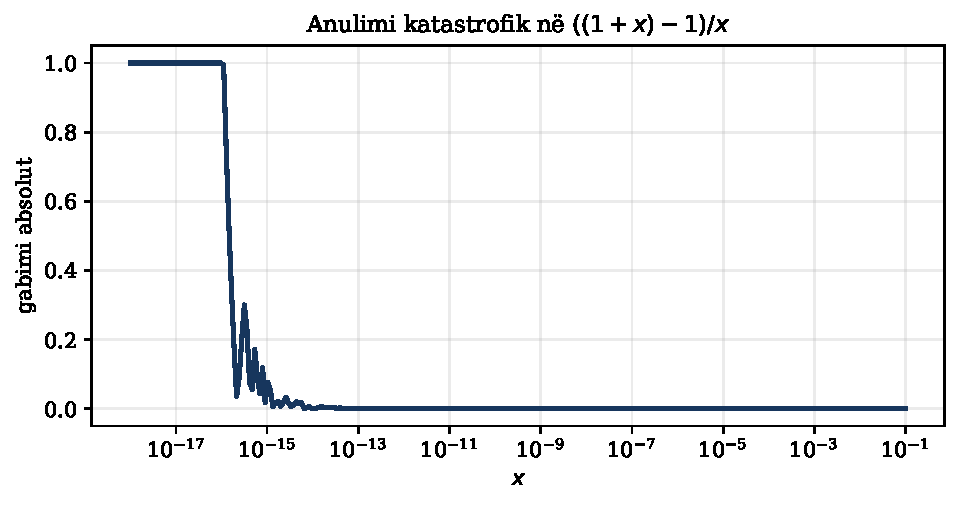
\includegraphics[width=.75\textwidth]{02_anulimi_katastrofik.pdf}
\caption{Gabimi i shkaktuar nga anulimi kur $x$ bëhet i krahasueshëm me saktësinë e makinës.}
\end{figure}

\begin{kujdes}
Renditja e veprimeve ka rëndësi. Në një shumë me terma me madhësi shumë të ndryshme, termat e vegjël mund të humbasin. Mbledhja nga moduli më i vogël te më i madhi ose algoritmi Kahan redukton humbjen.
\end{kujdes}

\section{Kushtëzimi i problemit}
Kushtëzimi është veti e problemit matematik. Për $y=f(x)$, numri relativ i kushtëzimit lokal është
\begin{equation}
 \kappa_f(x)=\left|\frac{x f'(x)}{f(x)}\right|.
\end{equation}
Në sistemin $A\vect x=\vect b$,
\begin{equation}
 \frac{\|\delta\vect x\|}{\|\vect x\|}\lesssim \kappa(A)\frac{\|\delta\vect b\|}{\|\vect b\|},
 \qquad \kappa(A)=\|A\|\,\|A^{-1}\|.
\end{equation}
Një matricë me $\kappa\gg1$ është e keqkushtëzuar: perturbime të vogla në të dhëna mund të prodhojnë ndryshime të mëdha në zgjidhje.

\begin{figure}[ht]
\centering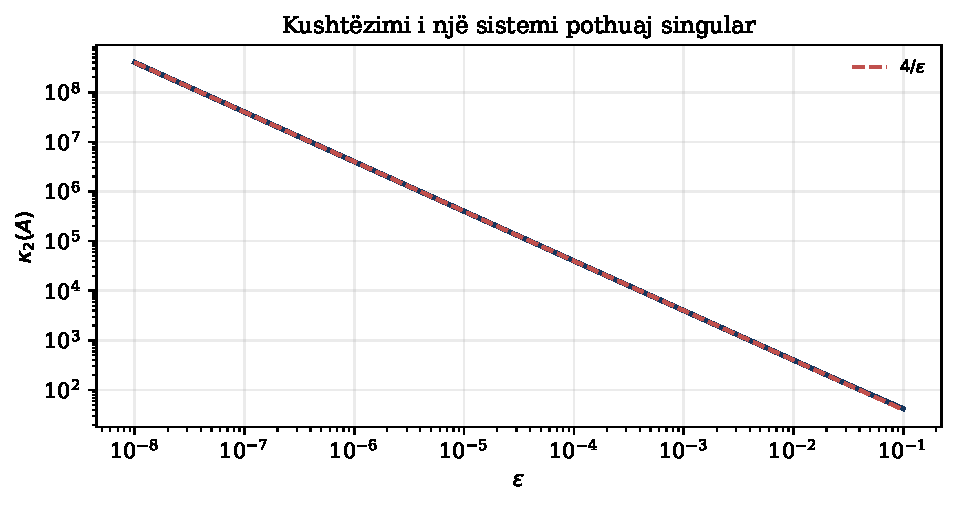
\includegraphics[width=.75\textwidth]{04_kushtzimi_matrices.pdf}
\caption{Rritja e numrit të kushtëzimit kur dy rreshta të matricës bëhen pothuaj linearë të varur.}
\end{figure}

\section{Gabimi i përparmë dhe i prapmë}
Gabimi i përparmë mat distancën ndërmjet rezultatit numerik dhe zgjidhjes së saktë. Analiza e prapme kërkon problemin pak të perturbur që zgjidhet saktësisht nga rezultati i llogaritur. Një algoritëm është i qëndrueshëm në kuptimin e prapëm nëse perturbimi i kërkuar është i vogël. Marrëdhënia konceptuale është
\begin{equation}
 \text{gabimi i përparmë}\ \lesssim\ \text{kushtëzimi}\times\text{gabimi i prapëm}.
\end{equation}
Prandaj, edhe algoritmi më i mirë nuk mund ta shpëtojë një problem intrinsikisht të keqkushtëzuar.

\section{Gabimet matricore}
Shumëzimi matricor kryen shumë mbledhje dhe shumëzime. Kufiri klasik për një produkt skalar me $n$ terma ka faktor
\begin{equation}
 \gamma_n=\frac{nu}{1-nu}\approx nu.
\end{equation}
Invertimi eksplicit i matricës për të zgjidhur $A\vect x=\vect b$ është zakonisht më i shtrenjtë dhe më pak i qëndrueshëm se faktorizimi i drejtpërdrejtë. Në kod përdoret operatori i zgjidhjes, jo $A^{-1}\vect b$.

\begin{shembull}[Shuma e energjive]
Nëse energjia totale merret si diferencë e dy energjive të mëdha, gabimi relativ mund të jetë i lartë edhe kur secila energji është llogaritur me shumë shifra. Një formulim që llogarit drejtpërdrejt madhësinë e vogël mund të jetë numerikisht më i sigurt.
\end{shembull}

\begin{lidhje}
Në laborator maten $u$, anulimi dhe ndikimi i rendit të mbledhjes. Pastaj ndërtohet një familje sistemesh $2\times2$ dhe krahasohet gabimi i zgjidhjes me $\kappa(A)$.
\end{lidhje}

\section*{Pyetje kontrolli}
\begin{enumerate}
\item Dalloni një problem të keqkushtëzuar nga një algoritëm i paqëndrueshëm.
\item Pse $A^{-1}\vect b$ nuk është mënyra e rekomanduar për të zgjidhur sistemin?
\item Jepni një reformulim që shmang anulimin katastrofik.
\end{enumerate}
\section{Algoritmet për diagnostikimin e gabimeve numerike}
Qëllimi praktik është të dallohen katër burime: gabimi i të dhënave, kushtëzimi i problemit, gabimi i algoritmit dhe rrumbullakimi. Një diagnozë e mirë ndryshon vetëm një faktor në çdo provë.

\subsection{Matja e saktësisë së makinës}
\begin{lstlisting}[language=Python,caption={Vlerësimi empirik i distancës pranë njësisë.}]
eps = 1.0
while 1.0 + eps/2.0 != 1.0:
    eps /= 2.0
print(eps, np.finfo(float).eps)
\end{lstlisting}
Vlera e marrë është epsilon-i i makinës sipas konventës së NumPy. Njësia e rrumbullakimit është afërsisht gjysma e saj.

\subsection{Shuma Kahan}
Në mbledhjen e shumë termave, një kompensim ruan pjesën e humbur nga rrumbullakimi.
\begin{lstlisting}[language=Python,caption={Mbledhja e kompensuar Kahan.}]
def shuma_kahan(x):
    s = 0.0
    c = 0.0
    for value in x:
        y = value - c
        t = s + y
        c = (t - s) - y
        s = t
    return s

x = np.r_[1e16, np.ones(1_000_000), -1e16]
print(np.sum(x), shuma_kahan(x))
\end{lstlisting}
Ky test duhet përsëritur me renditje të ndryshme. Rezultati tregon se asociativiteti algjebrik nuk ruhet plotësisht në pikë të lëvizshme.

\subsection{Kushtëzimi dhe mbetja}
\begin{lstlisting}[language=Python,caption={Krahasimi i gabimit me mbetjen.}]
def diagnostiko(A, b, x_ref):
    x = np.linalg.solve(A, b)
    mbetja = np.linalg.norm(b - A @ x) / np.linalg.norm(b)
    gabimi = np.linalg.norm(x - x_ref) / np.linalg.norm(x_ref)
    return np.linalg.cond(A), mbetja, gabimi

for e in [1e-2, 1e-6, 1e-10]:
    A = np.array([[1.0, 1.0], [1.0, 1.0 + e]])
    x_ref = np.array([1.0, 1.0])
    b = A @ x_ref
    print(e, diagnostiko(A, b, x_ref))
\end{lstlisting}
Mbetja mund të mbetet e vogël edhe kur gabimi i zgjidhjes rritet. Prandaj raportohen të dyja bashkë me $\kappa(A)$.

\subsection{Algoritmi i auditimit}
\begin{enumerate}
\item Përcaktohet një zgjidhje reference me saktësi të lartë ose analitike.
\item Ndryshohet hapi, toleranca ose rendi i veprimeve.
\item Vizatohet gabimi në shkallë logaritmike.
\item Kontrollohet pjerrësia e pritur e konvergjencës.
\item Përsëritet me të dhëna pak të perturbura për të matur kushtëzimin.
\end{enumerate}

Terminologjia \emph{gabim i përparmë}, \emph{gabim i prapëm}, \emph{kushtëzim} dhe \emph{qëndrueshmëri} përdoret sipas traditës së analizës numerike në shqip, veçanërisht në tekstet e Hanellit--Osmanit dhe Hoxhës.

Për trajtimin në shqip të gabimeve, sistemeve lineare dhe qëndrueshmërisë janë përdorur \cite{hanelli,hoxha,datja}; analiza moderne e qëndrueshmërisë krahasohet me \cite{higham}.

\subsection{Modeli standard i rrumbullakimit dhe përhapja e gabimit}
Le të jetë $\operatorname{fl}(x)$ numri i përfaqësueshëm më i afërt me $x$. Për numrat normalë dhe rrumbullakimin drejt më të afërtit shkruhet
\begin{equation}
 \operatorname{fl}(x)=x(1+\delta),\qquad |\delta|\le u.
\end{equation}
Ky model është relativ dhe prandaj nuk përshkruan drejtpërdrejt sjelljen pranë nënmbushjes. Për një varg veprimesh, çdo hap fut një faktor të ri $(1+\delta_i)$. Prodhimi plotëson
\begin{equation}
 \prod_{i=1}^{n}(1+\delta_i)=1+\theta_n,qquad
 |\theta_n|\le\gamma_n=\frac{nu}{1-nu},
\end{equation}
kur $nu<1$. Formula $\gamma_n\simeq nu$ është e dobishme, por nuk duhet interpretuar si parashikim i saktë i gabimit: ajo është kufi në rastin më të pafavorshëm.

Për $f(x_1,\ldots,x_p)$, linearizimi jep
\begin{equation}
 \Delta f\simeq\sum_{j=1}^{p}\frac{\partial f}{\partial x_j}\Delta x_j.
\end{equation}
Nëse perturbimet trajtohen si të pavarura me devijime standarde $\sigma_j$, përhapja probabilitare e rendit të parë është
\begin{equation}
 \sigma_f^2\simeq\sum_{j=1}^{p}\left(\frac{\partial f}{\partial x_j}\right)^2\sigma_j^2,
\end{equation}
ndërsa për hyrje të korreluara shfaqen termat $2(\partial_i f)(\partial_j f)\operatorname{Cov}(x_i,x_j)$. Analiza deterministe e rrumbullakimit dhe përhapja probabilitare e pacaktueshmërisë nuk janë e njëjta gjë, megjithëse përdorin të njëjtin mjet të linearizimit.

\subsection{Kushtëzimi absolut dhe relativ}
Për një hartë $f:\R^n\to\R^m$, perturbimi i rendit të parë është $\Delta\vect y\simeq J_f(\vect x)\Delta\vect x$. Numri absolut i kushtëzimit në normat e zgjedhura është
\begin{equation}
 \kappa_{\mathrm{abs}}(\vect x)=\|J_f(\vect x)\|,
\end{equation}
kurse numri relativ mund të shkruhet
\begin{equation}
 \kappa_{\mathrm{rel}}(\vect x)=
 \frac{\|J_f(\vect x)\|\,\|\vect x\|}{\|f(\vect x)\|}.
\end{equation}
Kjo formulë tregon pse kushtëzimi rritet pranë një rezultati zero: një ndryshim absolut i moderuar bëhet ndryshim relativ i madh. Për sistemin linear, nga
\begin{equation}
 (A+\Delta A)(\vect x+\Delta\vect x)=\vect b+\Delta\vect b
\end{equation}
dhe neglizhimi i produkteve të rendit të dytë merret
\begin{equation}
 A\Delta\vect x\simeq\Delta\vect b-\Delta A\vect x.
\end{equation}
Prandaj
\begin{equation}
 \frac{\|\Delta\vect x\|}{\|\vect x\|}
 \lesssim\kappa(A)\left(
 \frac{\|\Delta A\|}{\|A\|}+\frac{\|\Delta\vect b\|}{\|\vect b\|}
 \right),
\end{equation}
me kusht që perturbimi i matricës të jetë mjaft i vogël.

\subsection{Mbetja dhe kufiri i gabimit të zgjidhjes}
Për një përafrim $\widehat{\vect x}$, mbetja është $\vect r=\vect b-A\widehat{\vect x}$. Gabimi i vërtetë $\vect e=\vect x-\widehat{\vect x}$ plotëson $A\vect e=\vect r$, kështu që
\begin{equation}
 \|\vect e\|\le\|A^{-1}\|\,\|\vect r\|.
\end{equation}
Duke normalizuar dhe përdorur $\|\vect b\|\le\|A\|\|\vect x\|$ merret kufiri praktik
\begin{equation}
 \frac{\|\vect e\|}{\|\vect x\|}
 \le \kappa(A)\frac{\|\vect r\|}{\|\vect b\|}.
\end{equation}
Pra mbetja e vogël është e nevojshme, por jo e mjaftueshme për saktësi të lartë kur $\kappa(A)$ është e madhe.

\begin{lstlisting}[language=Python,caption={Raport diagnostik për një sistem linear.}]
import numpy as np

def raport_sistemi(A, b, x_hat):
    r = b - A @ x_hat
    mbetje_relative = np.linalg.norm(r) / np.linalg.norm(b)
    kappa = np.linalg.cond(A)
    kufi_gabimi = kappa * mbetje_relative
    return {"kappa": kappa,
            "mbetje_relative": mbetje_relative,
            "kufi_i_perafert": kufi_gabimi}
\end{lstlisting}
Funksioni nuk pretendon se kufiri është gabimi real; ai jep një alarm të arsyetuar. Në MATLAB/Octave përdoren \texttt{norm}, \texttt{cond} dhe prodhimi \texttt{A*x\_hat}.

\subsection{Përmbledhje dhe ushtrime}
Gabimi i të dhënave, kushtëzimi i problemit dhe qëndrueshmëria e algoritmit duhet të analizohen veçmas. Një raport numerik pa mbetje, kushtëzim dhe studim të saktësisë është i paplotë.
\begin{enumerate}
\item Nxirrni numrin relativ të kushtëzimit të $f(x)=1/(1-x)$ dhe interpretojeni pranë $x=1$.
\item Provoni kufirin $|\theta_n|\le\gamma_n$ për $n=2$ dhe diskutoni rolin e termit $u^2$.
\item Krahasoni shumën naive, shumën nga termi më i vogël dhe shumën Kahan për një varg me shkallë të ndryshme.
\item Ndërtoni matrica me numër kushtëzimi të kontrolluar nga vlerat singulare dhe studioni gabimin përpara.
\end{enumerate}

\subsection{Shuma, produkti skalar dhe gabimet e grumbulluara}
Shuma $s_n=\sum_{i=1}^{n}x_i$ duket operacion elementar, por është një nga burimet më të zakonshme të humbjes së saktësisë. Në mbledhjen naive,
\begin{equation}
 \widehat s_k=\operatorname{fl}(\widehat s_{k-1}+x_k),
\end{equation}
secili hap rrumbullakon rezultatin e pjesshëm. Analiza standarde jep
\begin{equation}
 |\widehat s_n-s_n|\le\gamma_{n-1}\sum_{i=1}^{n}|x_i|,
\end{equation}
ku $\gamma_{n-1}\simeq(n-1)u$. Kufiri varet nga shuma e moduleve, jo nga moduli i shumës. Kur ka anulim të fortë, $|s_n|\ll\sum|x_i|$, gabimi relativ mund të jetë i madh edhe pse gabimi absolut respekton kufirin.

Mbledhja në çift formon një pemë binare dhe ka thellësi $\lceil\log_2n\rceil$ në vend të $n-1$; kufiri përkatës rritet afërsisht me $u\log_2n$. Kjo është e rëndësishme në llogaritjen paralele, ku rendi i reduktimit ndryshon rezultatin bit për bit. Algoritmi Kahan ruan një kompensim për pjesën e humbur dhe shpesh arrin gabim të krahasueshëm me një rrumbullakim të vetëm, megjithëse nuk është ilaç universal për të gjitha vargjet.

Produkti skalar $\vect x^T\vect y$ kombinon shumëzime dhe mbledhje. Kufiri tipik është
\begin{equation}
 |\operatorname{fl}(\vect x^T\vect y)-\vect x^T\vect y|
 \le\gamma_n |\vect x|^T|\vect y|.
\end{equation}
Ky rezultat përhapet te shumëzimi matricor element për element. Në simulime të mëdha, ndryshimi i bibliotekës BLAS, numrit të threads ose rendit të ndarjes mund të ndryshojë bitat e fundit pa ndryshuar vlefshmërinë shkencore. Riprodhueshmëria duhet të përcaktojë nëse kërkohet identitet bit për bit apo vetëm pajtim brenda një tolerance.

\subsubsection{Kushtëzimi komponentor}
Numri klasik $\kappa(A)=\|A\|\|A^{-1}\|$ mat perturbime normore. Në disa probleme, hyrjet kanë pacaktueshmëri relative komponent më komponent. Atëherë një matricë me elemente në shkallë shumë të ndryshme mund të duket keq në një normë, edhe pse struktura fizike e perturbimeve është më e kufizuar. Analiza komponentore përdor $|\Delta A|\le\varepsilon|A|$ dhe $|\Delta b|\le\varepsilon|b|$. Ky dallim është me rëndësi në rrjete rezistive, sisteme bilanci dhe matrica që përmbajnë koeficientë me njësi të ndryshme.

Shkallëzimi me matrica diagonale $D_rAD_c$ mund të barazojë madhësitë e rreshtave dhe kolonave. Ai nuk ndryshon zgjidhjen fizike pasi ndryshoret rikthehen, por mund të përmirësojë sjelljen e eliminimit dhe kuptimin e tolerancave. Shkallëzimi nuk e shëron një varësi reale lineare; ai vetëm shmang që njësitë e papërshtatshme të duken si keqkushtëzim.

\subsubsection{Aritmetika e intervaleve si kontroll}
Në aritmetikën e intervaleve, një madhësi ruhet si $[a,b]$ që garanton përfshirjen e vlerës së saktë. Veprimet rrumbullakohen nga jashtë. Për shembull,
\begin{equation}
 [a,b]+[c,d]=[a+c,b+d].
\end{equation}
Avantazhi është një kufi i garantuar; kufizimi është mbivlerësimi nga varësia. Nëse $x\in[0,1]$, shprehja $x-x$ vlerësohet si $[-1,1]$, megjithëse është saktësisht zero, sepse dy paraqitjet e $x$ trajtohen si të pavarura. Aritmetika e intervaleve është e dobishme për verifikime lokale dhe kufij, por nuk zëvendëson analizën e kushtëzimit ose modelin probabilitar të pacaktueshmërisë.


\chapter{Ekuacionet jolineare, sistemet lineare dhe vlerat vetjake}
\begin{qellime}
Studenti zbaton përgjysmimin, pikën fikse, Njutonin dhe sekanten; zgjidh sisteme lineare me eliminim e faktorizim; interpreton kushtëzimin; llogarit vlera e vektorë vetjakë me metodën fuqi dhe algoritmin QR.
\end{qellime}

\section{Ekuacioni skalar $f(x)=0$}
Rrënja është pikë ku modeli plotëson një kusht fizik: ekuilibër force, energji e caktuar, kohë goditjeje ose parametër kalibrimi. Metoda duhet zgjedhur sipas informacionit të disponueshëm, intervalit të sigurt dhe kostos së vlerësimit të funksionit.

\subsection{Përgjysmimi}
Nëse $f$ është e vazhdueshme dhe $f(a)f(b)<0$, ekziston të paktën një rrënjë në $[a,b]$. Pas $n$ hapash,
\begin{equation}
 |x_n-x_*|\le \frac{b-a}{2^{n+1}}.
\end{equation}
Metoda është e ngadaltë, por robuste. Ajo nuk dallon rrënjët me shumëfish çift, sepse shenja mund të mos ndryshojë.

\begin{shembull}[Algoritmi i përgjysmimit]
Jepen $f$, $a$, $b$ dhe toleranca $\tau$, me $f(a)f(b)<0$. Për sa kohë $(b-a)/2>\tau$, vendoset $c=(a+b)/2$. Nëse $f(a)f(c)\le0$, zëvendësohet $b$ me $c$; përndryshe zëvendësohet $a$ me $c$. Në fund kthehet $(a+b)/2$.
\end{shembull}

\subsection{Pika fikse dhe Njutoni}
Shkrimi $x=g(x)$ jep iteracionin $x_{n+1}=g(x_n)$. Konvergjenca lokale kërkon $|g'(x_*)|<1$. Përzgjedhja e $g$ është pjesë e metodës; forma algjebrike e papërshtatshme mund të divergojë.

Linearizimi i $f$ rreth $x_n$ jep metodën e Njutonit,
\begin{equation}
 x_{n+1}=x_n-\frac{f(x_n)}{f'(x_n)}.
\end{equation}
Pranë një rrënje të thjeshtë, gabimi është kuadratik: $|e_{n+1}|\approx C|e_n|^2$. Megjithatë, derivati i vogël, pika fillestare e keqe ose dalja nga domeni mund ta dështojnë metodën. Një strategji praktike kombinon intervalin e përgjysmimit me hapin e Njutonit.

Sekantja zëvendëson derivatin me pjerrësinë ndërmjet dy pikave. Ajo nuk kërkon derivat dhe ka rend konvergjence $\varphi=(1+\sqrt5)/2$.

\begin{figure}[ht]
\centering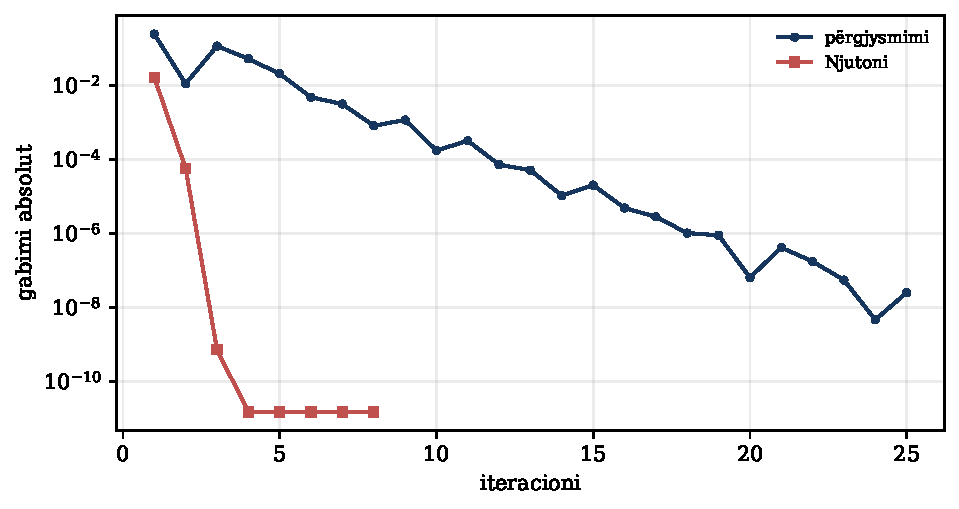
\includegraphics[width=.75\textwidth]{03_konvergjenca_rrenjeve.pdf}
\caption{Konvergjenca lineare e përgjysmimit dhe konvergjenca e shpejtë e Njutonit për $\cos x-x=0$.}
\end{figure}

\section{Sistemet jolineare}
Për $\vect F(\vect x)=\vect0$, linearizimi përdor Jakobin $J_{ij}=\partial F_i/\partial x_j$:
\begin{equation}
 J(\vect x_k)\Delta\vect x_k=-\vect F(\vect x_k),\qquad
 \vect x_{k+1}=\vect x_k+\Delta\vect x_k.
\end{equation}
Në çdo hap zgjidhet një sistem linear; inversi nuk formohet. Shkallëzimi i ndryshoreve është i rëndësishëm kur komponentët kanë njësi ose madhësi shumë të ndryshme. Në probleme të vështira përdoret amortizimi $\vect x_{k+1}=\vect x_k+\lambda\Delta\vect x_k$, $0<\lambda\le1$.

\begin{shembull}[Ekuilibri mekanik]
Për dy masa të lidhura me susta jolineare, $\vect F(\vect x)$ përmbledh forcat neto. Jakobiani është matrica e ngurtësisë tangjente. Konvergjenca e Njutonit tregon jo vetëm zgjidhjen, por edhe afërsinë ndaj humbjes së stabilitetit kur $J$ bëhet pothuaj singular.
\end{shembull}

\section{Sistemet lineare}
Eliminimi i Gausit e shndërron $A$ në formë trekëndore. Pivotimi i pjesshëm zgjedh elementin me modul më të madh në kolonën aktive dhe shmang pjesëtimin me numra të vegjël. Faktorizimi shkruhet
\begin{equation}
 PA=LU,
\end{equation}
ku $P$ është matricë permutimi, $L$ trekëndore e poshtme dhe $U$ trekëndore e sipërme. Për shumë anë të djathta, faktorizimi kryhet një herë dhe zëvendësimet përsëriten.

Për matrica simetrike pozitivisht të përcaktuara përdoret Cholesky,
\begin{equation}
 A=LL^T,
\end{equation}
që shfrytëzon simetrinë dhe ka rreth gjysmën e kostos së LU. Kostoja e faktorizimit të një matrice të dendur $n\times n$ është $\Oh(n^3)$; ruajtja është $\Oh(n^2)$.

\begin{kujdes}
Determinanti i vogël nuk është masë e mirë e kushtëzimit, sepse varet nga shkalla. Përdoret $\kappa(A)$ ose vlera singulare më e vogël. Gjithashtu, një mbetje e vogël $\vect r=\vect b-A\tilde{\vect x}$ nuk garanton gabim të vogël kur $A$ është e keqkushtëzuar.
\end{kujdes}

\section{Vlerat dhe vektorët vetjakë}
Problemi
\begin{equation}
 A\vect v=\lambda\vect v
\end{equation}
shfaqet në modet normale, stabilitet, mekanikë kuantike dhe analiza të rrjeteve. Për një sistem masë--sustë,
\begin{equation}
 K\vect u=\omega^2 M\vect u.
\end{equation}
Vektorët vetjakë janë format modale; vlerat vetjake japin frekuencat katrore.

\begin{figure}[ht]
\centering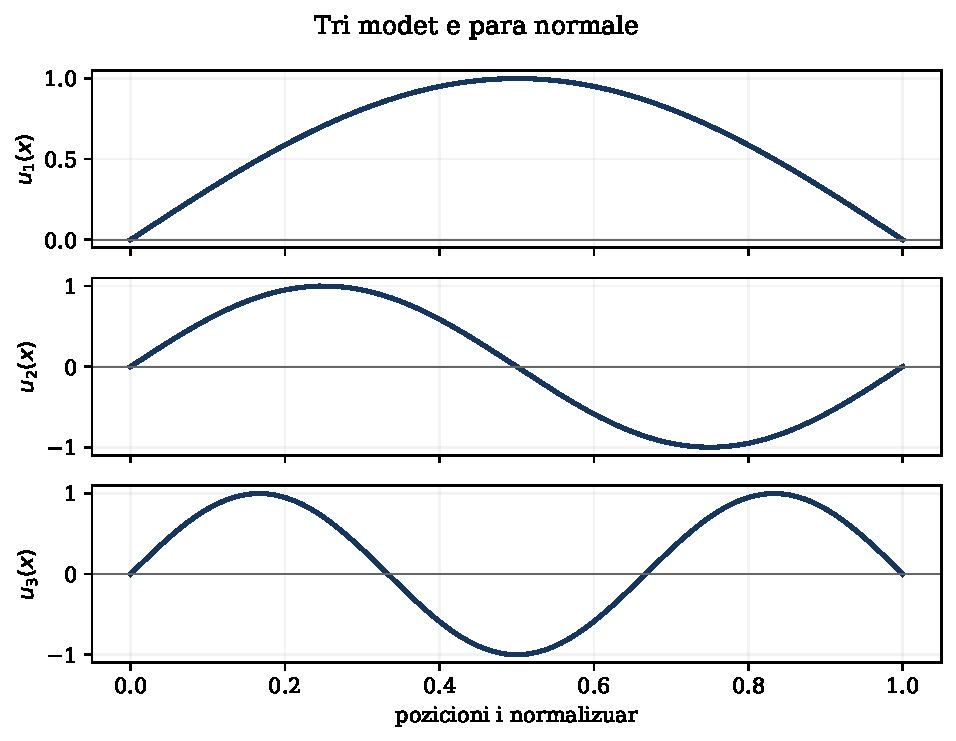
\includegraphics[width=.72\textwidth]{05_modet_normale.pdf}
\caption{Mode normale të një sistemi njëpërmasor me skaje të fiksuara.}
\end{figure}

\subsection{Metoda fuqi}
Iteracioni $\vect x_{k+1}=A\vect x_k/\|A\vect x_k\|$ izolon vektorin e lidhur me vlerën vetjake me modul më të madh, nëse komponenti fillestar përkatës nuk është zero. Shpejtësia përcaktohet nga $|\lambda_2/\lambda_1|$. Vlera vlerësohet me kuocientin Rayleigh
\begin{equation}
 \rho(\vect x)=\frac{\vect x^T A\vect x}{\vect x^T\vect x}.
\end{equation}

\subsection{Algoritmi QR}
Faktorizimi $A_k=Q_kR_k$ dhe përditësimi $A_{k+1}=R_kQ_k$ prodhojnë matrica të ngjashme, pra me të njëjtat vlera vetjake. Për matrica simetrike, $A_k$ afrohet drejt formës diagonale. Në praktikë përdoren reduktimi Hessenberg/tridiagonal dhe zhvendosjet për konvergjencë të shpejtë.

\section{Renditja e faqeve si problem vetjak}
Një matricë kalimi $P$ përshkruan probabilitetin e kalimit ndërmjet faqeve. Vektori stacionar plotëson $\vect p=P\vect p$. Faktori i amortizimit shmang nyjet pa dalje dhe komponentët e shkëputur:
\begin{equation}
 G=\alpha P+(1-\alpha)\frac{\vect1\vect1^T}{n}.
\end{equation}
Metoda fuqi mbi $G$ jep renditjen. Ky shembull lidh algjebrën lineare, zinxhirët Markov dhe simulimin.

\begin{lidhje}
Laboratori ndërton sistemin masë--sustë, verifikon simetrinë, llogarit frekuencat dhe vizaton modet. Një ushtrim shtesë ndërton një rrjet të vogël faqesh dhe krahason iteracionin e fuqisë me zgjidhjen e drejtpërdrejtë.
\end{lidhje}

\section*{Pyetje kontrolli}
\begin{enumerate}
\item Kur preferohet përgjysmimi ndaj Njutonit?
\item Pse pivotimi është pjesë e qëndrueshmërisë së eliminimit?
\item Çfarë përcakton shpejtësinë e metodës fuqi?
\end{enumerate}
\section{Algoritmet kryesore dhe zbatimi në Python}
Ky kapitull përmban tri familje problemesh. Secila kërkon një kriter ndalimi të lidhur me mbetjen, jo vetëm me ndryshimin ndërmjet dy iteracioneve.

\subsection{Përgjysmimi dhe Njutoni i mbrojtur}
\begin{lstlisting}[language=Python,caption={Përgjysmimi me kontroll të intervalit.}]
def pergjysmimi(f, a, b, tol=1e-12, max_iter=200):
    fa, fb = f(a), f(b)
    if fa * fb > 0:
        raise ValueError("Intervali nuk kufizon nje ndryshim shenje.")
    for _ in range(max_iter):
        c = 0.5 * (a + b)
        fc = f(c)
        if abs(fc) < tol or 0.5*(b-a) < tol:
            return c
        if fa * fc <= 0:
            b, fb = c, fc
        else:
            a, fa = c, fc
    raise RuntimeError("Nuk u arrit konvergjenca.")
\end{lstlisting}

\begin{lstlisting}[language=Python,caption={Njutoni me kontroll të derivatit.}]
def njutoni(f, df, x, tol=1e-12, max_iter=50):
    for _ in range(max_iter):
        fx, dfx = f(x), df(x)
        if abs(fx) < tol:
            return x
        if abs(dfx) < np.sqrt(np.finfo(float).eps):
            raise ArithmeticError("Derivat shume i vogel.")
        hapi = -fx / dfx
        x = x + hapi
        if abs(hapi) < tol * (1 + abs(x)):
            return x
    raise RuntimeError("Nuk u arrit konvergjenca.")
\end{lstlisting}
Në një zbatim robust, hapi i Njutonit pranohet vetëm nëse qëndron brenda intervalit dhe zvogëlon mbetjen; përndryshe kryhet një përgjysmim.

\subsection{Zgjidhja e sistemit linear}
\begin{lstlisting}[language=Python,caption={Zgjidhja dhe diagnostika pa formuar inversin.}]
A = np.array([[4., -1., 0.], [-1., 4., -1.], [0., -1., 3.]])
b = np.array([15., 10., 10.])
x = np.linalg.solve(A, b)
r = b - A @ x
print("x =", x)
print("mbetja relative =", np.linalg.norm(r)/np.linalg.norm(b))
print("kappa_2 =", np.linalg.cond(A))
\end{lstlisting}
Operatori \texttt{solve} përdor faktorizime të përshtatshme. Shkrimi \texttt{inv(A) @ b} shmanget.

\subsection{Metoda fuqi}
\begin{lstlisting}[language=Python,caption={Vlera vetjake dominante dhe kuocienti Rayleigh.}]
def metoda_fuqi(A, tol=1e-11, max_iter=10_000):
    x = np.ones(A.shape[0])
    x /= np.linalg.norm(x)
    lam_old = 0.0
    for k in range(max_iter):
        y = A @ x
        x = y / np.linalg.norm(y)
        lam = x @ A @ x
        if abs(lam - lam_old) < tol * (1 + abs(lam)):
            return lam, x, k + 1
        lam_old = lam
    raise RuntimeError("Metoda fuqi nuk konvergoi.")
\end{lstlisting}
Kontrolli përfundimtar është norma $\|A\vect x-\lambda\vect x\|$. Shenja e vektorit vetjak nuk ka kuptim fizik më vete: $\vect x$ dhe $-\vect x$ përfaqësojnë të njëjtin mod.

\subsection{Lidhja me modet normale}
Për $K\vect u=\omega^2M\vect u$, përdoret \texttt{scipy.linalg.eigh(K, M)} kur $K$ dhe $M$ janë simetrike dhe $M$ pozitivisht e përcaktuar. Frekuencat renditen, normalizohen dhe kontrollohet ortogonaliteti $U^TMU=I$.

Rendi i paraqitjes së metodave të rrënjëve, sistemeve dhe vlerave vetjake ndjek traditën e teksteve shqip \cite{hanelli,hoxha,datja}; termat e algjebrës lineare numerike kontrollohen edhe kundrejt punimeve të Departamentit të Matematikës së Aplikuar të UT-së \cite{zeqiri2020}.

\subsection{Konvergjenca e metodave për rrënjët}
Le të jetë $x_*$ rrënjë e thjeshtë. Në iteracionin e pikës fikse $x_{k+1}=g(x_k)$, teorema e vlerës mesatare jep
\begin{equation}
 e_{k+1}=x_{k+1}-x_*=g'(\xi_k)(x_k-x_*)=g'(\xi_k)e_k.
\end{equation}
Nëse $|g'(x)|\le q<1$ në një interval që ruhet nga $g$, atëherë $|e_k|\le q^k|e_0|$. Ky është konvergjim linear. Për Njutonin, zhvillimi Taylor rreth $x_k$ jep
\begin{equation}
 0=f(x_*)=f(x_k)+f'(x_k)(x_*-x_k)+\frac{f''(\xi_k)}{2}(x_*-x_k)^2.
\end{equation}
Pas zëvendësimit të hapit të Njutonit merret
\begin{equation}
 e_{k+1}=\frac{f''(\xi_k)}{2f'(x_k)}e_k^2.
\end{equation}
Konvergjenca kuadratike vlen vetëm pasi iteracioni ka hyrë në fqinjësinë e rrënjës dhe kur $f'(x_*)\ne0$. Për një rrënjë me shumëfish $m$, Njutoni standard bëhet linear; formula e modifikuar $x_{k+1}=x_k-mf(x_k)/f'(x_k)$ rikthen rendin kuadratik kur $m$ dihet.

Metoda e Müller-it ndërton një polinom kuadratik në tri pika dhe zgjedh rrënjën e tij që vazhdon trajektoren e iteracionit. Ajo mund të prodhojë rrënjë komplekse edhe nga pika fillestare reale, çka është avantazh për polinomet, por kërkon trajtim të kujdesshëm të degës së rrënjës katrore dhe të anulimit në emërues.

\subsection{Eliminimi i Gausit dhe pivotimi}
Në hapin $k$, elementi $a_{kk}^{(k)}$ përdoret si pivot dhe shumëzuesit janë
\begin{equation}
 \ell_{ik}=\frac{a_{ik}^{(k)}}{a_{kk}^{(k)}},\qquad i=k+1,\ldots,n.
\end{equation}
Rreshti $i$ përditësohet me $a_{ij}^{(k+1)}=a_{ij}^{(k)}-\ell_{ik}a_{kj}^{(k)}$. Në aritmetikë të saktë, kjo është një sekuencë transformimesh elementare. Në aritmetikë me saktësi të fundme, pivot i vogël prodhon shumëzues të mëdhenj dhe zmadhon gabimet. Pivotimi i pjesshëm zgjedh
\begin{equation}
 p=\arg\max_{i\ge k}|a_{ik}^{(k)}|
\end{equation}
dhe këmben rreshtat $p$ dhe $k$. Rezultati ruhet si $PA=LU$. Faktorizimi kushton afërsisht $2n^3/3$ veprime me presje të lëvizshme, kurse dy zëvendësimet për çdo anë të djathtë kushtojnë $\Oh(n^2)$.

Formimi i $A^{-1}$ kërkon zgjidhjen e $n$ sistemeve dhe pastaj një shumëzim tjetër me $\vect b$; ai shton punë dhe rrumbullakime pa nevojë. Për këtë arsye \texttt{solve(A,b)} është zgjedhja standarde.

\subsection{Njutoni për sisteme dhe kriteret e ndalimit}
Nga zhvillimi shumëpërmasor
\begin{equation}
 \vect F(\vect x+\Delta\vect x)=\vect F(\vect x)+J(\vect x)\Delta\vect x+\Oh(\|\Delta\vect x\|^2)
\end{equation}
vendosja e anës së majtë në zero jep sistemin e Njutonit. Duhet të kontrollohen njëkohësisht norma e mbetjes dhe madhësia relative e hapit,
\begin{equation}
 \|\vect F(\vect x_k)\|\le\tau_F,
 \qquad
 \|\Delta\vect x_k\|\le\tau_x(1+\|\vect x_k\|).
\end{equation}
Vetëm kriteri i hapit mund të pranojë stagnim; vetëm mbetja mund të mashtrojë kur ekuacionet kanë shkallë shumë të ndryshme. Shkallëzimi i secilit ekuacion me një madhësi karakteristike i bën kriteret fizikisht të krahasueshme.

\begin{lstlisting}[language=Python,caption={Njutoni i amortizuar për një sistem jolinear.}]
import numpy as np

def njutoni_sistem(F, J, x0, tol=1e-10, maksimumi=50):
    x = np.array(x0, dtype=float)
    for k in range(maksimumi):
        Fx = np.asarray(F(x), dtype=float)
        if np.linalg.norm(Fx, ord=np.inf) <= tol:
            return x, k
        hapi = np.linalg.solve(J(x), -Fx)
        alfa = 1.0
        # Kërkim prapa: pranohet vetëm ulja e normës së mbetjes.
        while np.linalg.norm(F(x + alfa*hapi)) >= np.linalg.norm(Fx):
            alfa *= 0.5
            if alfa < 2.0**-20:
                raise RuntimeError("Njutoni stagnoi; kontrolloni shkallëzimin.")
        x = x + alfa*hapi
    raise RuntimeError("U arrit numri maksimal i iteracioneve.")
\end{lstlisting}

\subsection{Metoda fuqi dhe algoritmi QR: derivim spektral}
Nëse $A$ ka një bazë vektorësh vetjakë dhe $\vect x_0=\sum_i c_i\vect v_i$, atëherë
\begin{equation}
 A^k\vect x_0=\lambda_1^k\left[c_1\vect v_1+
 \sum_{i=2}^{n}c_i\left(\frac{\lambda_i}{\lambda_1}\right)^k\vect v_i\right].
\end{equation}
Kur $|\lambda_1|>|\lambda_2|$ dhe $c_1\ne0$, termat e tjerë shuhen relativisht si $|\lambda_2/\lambda_1|^k$. Normalizimi shmang tejmbushjen, por nuk ndryshon drejtimin.

Në algoritmin QR, $A_k=Q_kR_k$ dhe $A_{k+1}=R_kQ_k=Q_k^TA_kQ_k$, kështu që $A_{k+1}$ është e ngjashme me $A_k$. Për matrica simetrike, transformimet ortogonale ruajnë mirë normën dhe diagonalja konvergon te vlerat vetjake. Zhvendosja $A_k-\mu_kI=Q_kR_k$, e ndjekur nga $A_{k+1}=R_kQ_k+\mu_kI$, përshpejton ndarjen e vlerave të afërta.

\subsection{Përmbledhje dhe ushtrime}
Metodat e këtij kapitulli bashkohen nga linearizimi: Njutoni linearizon funksionin, eliminimi zgjidh problemin linear dhe analiza spektrale shpjegon mënyrën si vepron matrica në drejtime të veçanta.
\begin{enumerate}
\item Nxirrni rendin e sekantes duke supozuar $|e_{k+1}|\simeq C|e_k e_{k-1}|$.
\item Implementoni Müller-in me numra kompleksë dhe provojeni te $x^4+1=0$.
\item Numëroni veprimet e eliminimit të Gausit dhe nxirrni termin $2n^3/3$.
\item Për një sistem masë--sustë, verifikoni ortogonalitetin e modeve ndaj matricës së masës.
\item Ndërtoni një rrjet faqesh dhe studioni ndikimin e parametrit të amortizimit në konvergjencën e renditjes.
\end{enumerate}

\subsection{Metoda e Müller-it dhe rrënjët komplekse}
Metoda e Müller-it përdor tri pika $x_0,x_1,x_2$ dhe ndërton polinomin kuadratik interpolues për $f$. Duke vendosur $h_1=x_1-x_0$, $h_2=x_2-x_1$ dhe diferencat e pjesëtuara
\begin{equation}
 \delta_1=\frac{f(x_1)-f(x_0)}{h_1},\qquad
 \delta_2=\frac{f(x_2)-f(x_1)}{h_2},
\end{equation}
koeficienti kuadratik është $d=(\delta_2-\delta_1)/(h_1+h_2)$. Polinomi rreth $x_2$ shkruhet
\begin{equation}
 p(x_2+s)=f(x_2)+bs+ds^2,qquad b=\delta_2+h_2d.
\end{equation}
Rrënja që jep hapin më të qëndrueshëm është
\begin{equation}
 s=-\frac{2f(x_2)}{b+\operatorname{sgn}_*(b)\sqrt{b^2-4df(x_2)}},
\end{equation}
ku shenja zgjidhet që emëruesi të ketë modul maksimal. Kjo zgjedhje shmang anulimin ndërmjet $b$ dhe rrënjës katrore. Pika e re është $x_3=x_2+s$, pastaj ruhet tresha më e fundit.

Diskriminanti mund të jetë negativ edhe kur pikat janë reale, prandaj implementimi duhet të lejojë aritmetikë komplekse. Kjo e bën Müller-in të dobishëm për polinome pa rrënjë reale. Renditja e konvergjencës është afërsisht $1.84$, më e lartë se e sekantes, por çdo hap përdor më shumë informacion dhe mund të jetë më pak i parashikueshëm. Për probleme ku kërkohet një rrënjë reale brenda një intervali fizik, një metodë e mbrojtur me përgjysmim është zakonisht më e sigurt.

\subsubsection{Refinimi iterativ i sistemeve lineare}
Pas zgjidhjes së $A\widehat x=b$, llogaritet mbetja $r=b-A\widehat x$ dhe zgjidhet
\begin{equation}
 A\delta x=r,qquad \widehat x\leftarrow\widehat x+\delta x.
\end{equation}
Në aritmetikë të saktë, një hap do të korrigjonte të gjithë gabimin. Në praktikë, nëse mbetja llogaritet me saktësi më të lartë se faktorizimi, refinimi mund të rikuperojë disa shifra. Faktorizimi LU ripërdoret, kështu që çdo korrigjim kushton vetëm dy zëvendësime trekëndore. Procesi ndalet kur mbetja e shkallëzuar nuk ulet më ose korrigjimi bëhet i papërfillshëm.

Një kriter i dobishëm komponentor është
\begin{equation}
 \eta=\max_i\frac{|r_i|}{(|A||\widehat x|+|b|)_i}.
\end{equation}
Ai interpretohet si perturbimi relativ minimal i afërt i të dhënave që e bën $\widehat x$ zgjidhje të saktë. Një $\eta$ pranë saktësisë së makinës tregon algoritëm të qëndrueshëm në prapavijë, por gabimi përpara mund të mbetet i madh kur sistemi është i keqkushtëzuar.

\subsubsection{Problemi i përgjithësuar i vlerave vetjake}
Në mekanikën e sistemeve me shumë shkallë lirie shfaqet
\begin{equation}
 K\vect u=\omega^2M\vect u,
\end{equation}
ku $M$ është matrica e masës dhe $K$ matrica e ngurtësisë. Nëse $M$ është simetrike pozitivisht e përcaktuar, faktorizimi Cholesky $M=LL^T$ e kthen problemin në
\begin{equation}
 L^{-1}KL^{-T}\vect z=\omega^2\vect z,qquad \vect u=L^{-T}\vect z.
\end{equation}
Matrica e transformuar është simetrike. Modet mund të normalizohen që $\vect u_i^TM\vect u_j=\delta_{ij}$ dhe atëherë $\vect u_i^TK\vect u_j=\omega_i^2\delta_{ij}$. Këto identitete janë prova numerike: mbetja $\|K\vect u_i-\omega_i^2M\vect u_i\|$ kontrollon çdo çift vetjak, ndërsa ortogonaliteti kontrollon të gjithë bazën.

Në rrjete ose sisteme me simetri, vlera vetjake të shumëfishta nuk përcaktojnë vektorë unikë; përcaktohet vetëm nënhapësira vetjake. Krahasimi komponent më komponent i dy vektorëve nga programe të ndryshme mund të jetë i pakuptimtë. Duhet krahasuar mbetja, vlera vetjake dhe hapësira e shtrirë nga modet përkatëse.


\chapter{Interpolimi, regresi dhe përshtatja e modeleve}
\begin{qellime}
Studenti ndërton polinomin e Lagranzhit dhe interpolimin Hermitian; dallon interpolimin nga regresi; zbaton katrorët më të vegjël linearë e jolinearë; interpreton mbetjet, peshat dhe pacaktueshmërinë e parametrave.
\end{qellime}

\section{Interpolimi polinomial}
Për nyje të dallueshme $(x_i,y_i)$ ekziston një polinom unik me gradë jo më të madhe se $n$ që kalon në $n+1$ pika. Forma e Lagranzhit është
\begin{equation}
 p_n(x)=\sum_{i=0}^{n}y_iL_i(x),\qquad
 L_i(x)=\prod_{j\ne i}\frac{x-x_j}{x_i-x_j}.
\end{equation}
Gabimi për $f\in C^{n+1}$ është
\begin{equation}
 f(x)-p_n(x)=\frac{f^{(n+1)}(\xi)}{(n+1)!}\prod_{i=0}^{n}(x-x_i).
\end{equation}
Formula tregon rolin e lëmueshmërisë dhe të vendosjes së nyjeve. Rritja e gradës në nyje të baraslarguara mund të përkeqësojë përafrimin pranë skajeve: fenomeni Runge.

\begin{figure}[ht]
\centering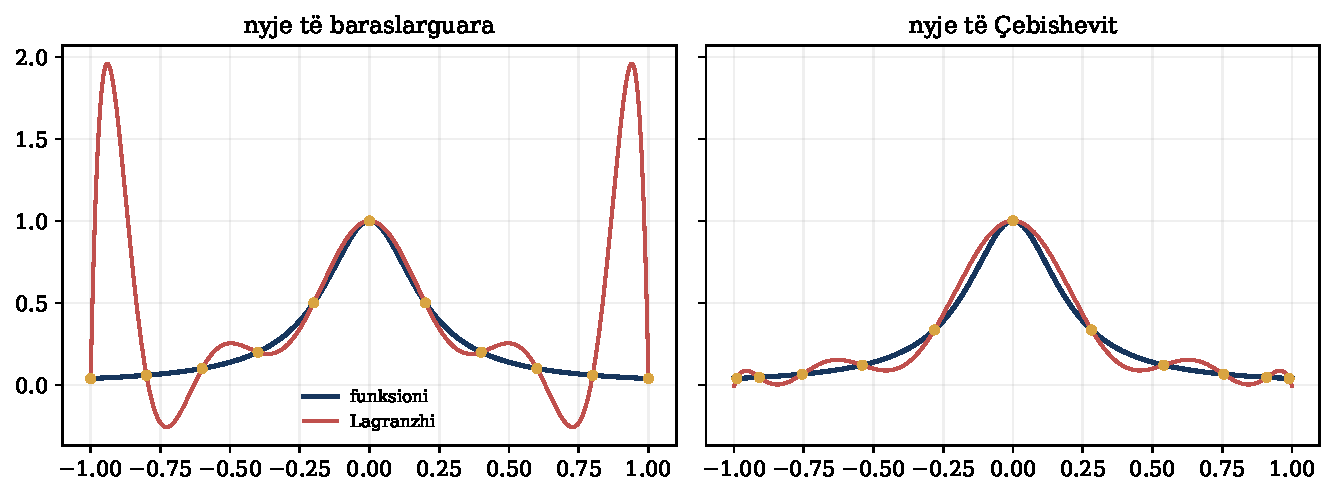
\includegraphics[width=.95\textwidth]{06_interpolimi_runge.pdf}
\caption{Interpolimi i funksionit Runge. Nyjet e Çebishevit zvogëlojnë lëkundjet në skaje.}
\end{figure}

Në llogaritje përdoret forma baricentrike, jo prodhimi i drejtpërdrejtë i polinomeve bazë. Për grupe të mëdha të dhënash preferohen splinet kubike, të cilat përdorin polinome lokale dhe ruajnë vazhdimësinë e dy derivateve të para.

\section{Interpolimi Hermitian dhe ekstrapolimi}
Interpolimi Hermitian përdor edhe vlerat e derivateve. Për dy pika, polinomi kubik përcaktohet nga $f(x_0)$, $f'(x_0)$, $f(x_1)$ dhe $f'(x_1)$. Kjo është bazë për trajektore të lëmuara dhe skema integrimi.

Ekstrapolimi vlerëson jashtë intervalit të të dhënave dhe është shumë më i rrezikshëm. Ekstrapolimi Richardson shfrytëzon një zhvillim të njohur të gabimit,
\begin{equation}
 A(h)=A+c h^p+\Oh(h^{p+1}),qquad
 A\approx\frac{2^pA(h/2)-A(h)}{2^p-1}.
\end{equation}
Ai përdoret për të rritur rendin ose për të vlerësuar kufirin $h\to0$.

\section{Regresi linear}
Në regres, pikat nuk kërkohet të kalohen saktësisht. Modeli $\vect y=X\vect\beta+\vect\varepsilon$ përshtatet duke minimizuar
\begin{equation}
 S(\vect\beta)=\|X\vect\beta-\vect y\|_2^2.
\end{equation}
Ekuacionet normale janë $X^TX\hat{\vect\beta}=X^T\vect y$, por formimi i $X^TX$ katrorëzon numrin e kushtëzimit. Faktorizimi QR është më i qëndrueshëm. Kur devijimet standarde $\sigma_i$ njihen, minimizohet
\begin{equation}
 \chi^2=\sum_i\frac{[y_i-f(x_i;\vect\beta)]^2}{\sigma_i^2}.
\end{equation}

\begin{figure}[ht]
\centering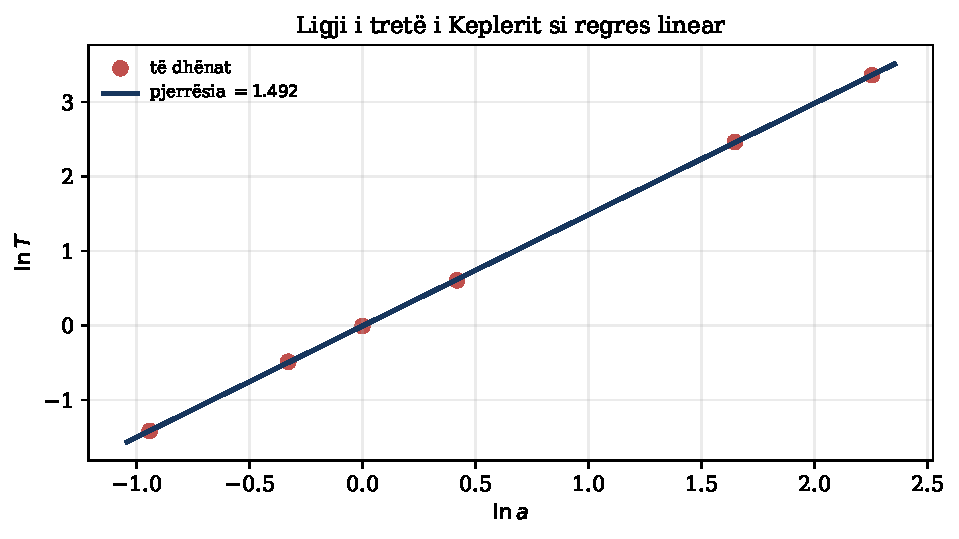
\includegraphics[width=.72\textwidth]{07_regresioni_kepler.pdf}
\caption{Linearizimi logaritmik i $T^2\propto a^3$. Pjerrësia e pritur për $\ln T$ kundrejt $\ln a$ është $3/2$.}
\end{figure}

\begin{shembull}[Ligji i tretë i Keplerit]
Modeli $T=C a^p$ bëhet $\ln T=\ln C+p\ln a$. Përshtatja jep $p$ dhe pacaktueshmërinë e tij. Transformimi logaritmik ndryshon strukturën e gabimit; nëse gabimi është aditiv në $T$, përshtatja jolineare në shkallën origjinale mund të jetë më e përshtatshme.
\end{shembull}

\section{Mbetjet dhe diagnostika}
Mbetjet $r_i=y_i-\hat y_i$ nuk janë mbeturina; ato testojnë modelin. Një strukturë sistematike në $r_i$ tregon jolinearitet të munguar, heteroskedasticitet, korrelacion ose pikë jashtë modelit. Koeficienti $R^2$ nuk mjafton për vleftësim dhe nuk duhet përdorur si provë shkakësie.

Për gabime Gauss të pavarura me variancë $\sigma^2$, kovarianca e parametrave është afërsisht
\begin{equation}
 \Cov(\hat{\vect\beta})=\sigma^2(X^TX)^{-1}.
\end{equation}
Në modele jolineare përdoret Jakobiani në optimum, bootstrap-i ose kampionimi probabilitar.

\section{Shmangiet minimale absolute}
Minimizimi $\sum_i|r_i|$ është më robust ndaj pikave ekstreme se katrorët më të vegjël. Funksioni nuk është i derivueshëm në zero, por problemi mund të formulohet si program linear. Zgjedhja e humbjes shpreh një supozim statistik: $L_2$ lidhet me gabimin Gauss, ndërsa $L_1$ me shpërndarje me bishta më të rëndë.

\begin{lidhje}
Laboratori përdor të dhëna planetare, përshtat $T=C a^p$, vizaton mbetjet dhe krahason regresin e papeshuar, të peshuar dhe një përshtatje robuste.
\end{lidhje}

\section*{Pyetje kontrolli}
\begin{enumerate}
\item Pse interpolimi me gradë të lartë mund të dështojë edhe për funksion të lëmuar?
\item Kur linearizimi logaritmik ndryshon interpretimin statistik të gabimit?
\item Çfarë informacioni japin mbetjet që nuk e jep $R^2$?
\end{enumerate}
\section{Algoritmet e interpolimit dhe përshtatjes}
\subsection{Interpolimi baricentrik}
Forma baricentrike është më e qëndrueshme se vlerësimi i drejtpërdrejtë i bazës së Lagranzhit. Peshat janë
\begin{equation}
 w_i=\left[\prod_{j\ne i}(x_i-x_j)\right]^{-1},\qquad
 p(x)=\frac{\sum_iw_iy_i/(x-x_i)}{\sum_iw_i/(x-x_i)}.
\end{equation}
Nëse $x$ përputhet me një nyje, kthehet drejtpërdrejt $y_i$.

\begin{lstlisting}[language=Python,caption={Interpolimi baricentrik nga SciPy.}]
import numpy as np
from scipy.interpolate import BarycentricInterpolator

f = lambda x: 1.0/(1.0 + 25.0*x*x)
n = 15
i = np.arange(n)
x_cheb = np.cos((2*i + 1)*np.pi/(2*n))
interp = BarycentricInterpolator(x_cheb, f(x_cheb))

x = np.linspace(-1, 1, 1000)
gabimi = np.max(np.abs(interp(x) - f(x)))
print("gabimi maksimal =", gabimi)
\end{lstlisting}

\subsection{Katrorët më të vegjël me QR}
\begin{lstlisting}[language=Python,caption={Përshtatja e një modeli linear në parametra.}]
def pershtat_linearisht(X, y, sigma=None):
    if sigma is not None:
        W = 1.0 / np.asarray(sigma)
        X = X * W[:, None]
        y = y * W
    beta, mbetje, rank, singular = np.linalg.lstsq(X, y, rcond=None)
    return beta, mbetje, rank, singular

# ln(T) = beta0 + beta1 ln(a)
X = np.column_stack([np.ones_like(a), np.log(a)])
beta, *_ = pershtat_linearisht(X, np.log(T))
print("eksponenti i Keplerit =", beta[1])
\end{lstlisting}
\texttt{lstsq} përdor faktorizime numerikisht më të sigurta se zgjidhja eksplicite e ekuacioneve normale.

\subsection{Përshtatja jolineare}
\begin{lstlisting}[language=Python,caption={Përshtatja e modelit $T=C a^p$ në shkallën origjinale.}]
from scipy.optimize import curve_fit

def kepler(a, C, p):
    return C * a**p

param, kov = curve_fit(kepler, a, T, p0=(1.0, 1.5), sigma=sigma_T,
                       absolute_sigma=True)
gabim_param = np.sqrt(np.diag(kov))
print(param, gabim_param)
\end{lstlisting}

\subsection{Diagnostika e mbetjeve}
Pas përshtatjes vizatohen $r_i$ kundrejt $x_i$, histogrami dhe, kur rendi kohor ka rëndësi, autokorrelacioni. Një lakim sistematik tregon model të mangët; formë hinke tregon variancë jo të njëtrajtshme; pika me ndikim të madh kërkojnë kontroll fizik, jo fshirje automatike.

\begin{kujdes}
Termi \emph{përshtatje} përdoret për fitting, \emph{mbetje} për residual dhe \emph{shmangie minimale absolute} për least absolute deviations. \emph{Regres} i referohet modelit të statistikës, ndërsa \emph{interpolim} kalon saktësisht nëpër nyje.
\end{kujdes}

Për interpolimin, përafrimin dhe shembujt MATLAB/Python janë konsultuar \cite{hanelli,hoxha,datja}. Për terminologjinë e rizgjedhjes, mbetjeve dhe vlerësimit statistik janë përdorur edhe punimet doktorale të UT-së \cite{butka,tasho}.

\subsection{Interpolimi i Lagranzhit dhe termi i mbetjes}
Për nyje të ndryshme $x_0,\ldots,x_n$, polinomi interpolues është
\begin{equation}
 p_n(x)=\sum_{i=0}^{n}f(x_i)L_i(x),\qquad
 L_i(x)=\prod_{j\ne i}\frac{x-x_j}{x_i-x_j}.
\end{equation}
Vërtetimi është i drejtpërdrejtë: $L_i(x_j)=\delta_{ij}$, prandaj $p_n(x_j)=f(x_j)$. Uniciteti rrjedh sepse diferenca e dy polinomeve interpoluese do të kishte $n+1$ rrënjë, por gradë jo më të madhe se $n$.

Nëse $f\in C^{n+1}$, gabimi në një pikë $x$ është
\begin{equation}
 f(x)-p_n(x)=\frac{f^{(n+1)}(\xi_x)}{(n+1)!}
 \omega_{n+1}(x),\qquad
 \omega_{n+1}(x)=\prod_{i=0}^{n}(x-x_i).
\end{equation}
Kjo formulë ndan dy burime: lëmueshmërinë e funksionit dhe gjeometrinë e nyjeve. Nyjet e baraslarguara mund ta bëjnë $\omega_{n+1}$ shumë të madhe pranë skajeve; nyjet e Çebishevit e kontrollojnë këtë faktor dhe zbusin dukurinë Runge.

Forma baricentrike
\begin{equation}
 p_n(x)=\frac{\sum_i w_i f_i/(x-x_i)}{\sum_i w_i/(x-x_i)},
 \qquad w_i=\left[\prod_{j\ne i}(x_i-x_j)\right]^{-1},
\end{equation}
është numerikisht më e përshtatshme se zgjerimi i polinomit në fuqi. Nëse $x$ përkon me një nyje, kthehet drejtpërdrejt $f_i$ për të shmangur pjesëtimin me zero.

\subsection{Interpolimi Hermitian dhe ekstrapolimi i Richardson-it}
Interpolimi Hermitian përdor jo vetëm $f(x_i)$, por edhe derivate. Për dy nyje dhe vlera të derivateve ndërtohet një polinom kub. Në formë të përgjithshme, nyjet përsëriten në tabelën e diferencave të pjesëtuara dhe diferenca e parë në një nyje të përsëritur zëvendësohet nga $f'(x_i)$.

Ekstrapolimi nis nga një përafrim me zhvillim asimptotik
\begin{equation}
 A(h)=A+c_ph^p+c_{p+1}h^{p+1}+\cdots.
\end{equation}
Dy vlera me hapa $h$ dhe $h/r$ japin
\begin{equation}
 A_{\mathrm{R}}=\frac{r^pA(h/r)-A(h)}{r^p-1}
 =A+\Oh(h^{p+1}),
\end{equation}
ose rend edhe më të lartë kur zhvillimi përmban vetëm fuqi çifte. Kjo është ideja pas derivimit të përmirësuar dhe integrimit Romberg. Ekstrapolimi nuk duhet zbatuar jashtë regjimit asimptotik; nëse hapi është shumë i madh, modeli i gabimit nuk vlen, ndërsa për hap tepër të vogël dominon rrumbullakimi.

\subsection{Katrorët më të vegjël dhe QR}
Për modelin linear $\vect y=X\vect\beta+\vect\varepsilon$, minimizohet
\begin{equation}
 S(\vect\beta)=\|\vect y-X\vect\beta\|_2^2.
\end{equation}
Gradienti është $\nabla S=-2X^T(\vect y-X\vect\beta)$. Kushti $\nabla S=0$ jep ekuacionet normale
\begin{equation}
 X^TX\widehat{\vect\beta}=X^T\vect y.
\end{equation}
Gjeometrikisht, mbetja është ortogonale me hapësirën e kolonave të $X$. Megjithatë, $\kappa(X^TX)=\kappa(X)^2$, prandaj formimi i ekuacioneve normale përkeqëson kushtëzimin. Me $X=QR$, ku $Q^TQ=I$, zgjidhet
\begin{equation}
 R\widehat{\vect\beta}=Q^T\vect y,
\end{equation}
pa katrorëzuar numrin e kushtëzimit.

Nëse gabimet kanë kovariancë $\Sigma$, kriteri i peshuar është
\begin{equation}
 (\vect y-X\vect\beta)^T\Sigma^{-1}(\vect y-X\vect\beta).
\end{equation}
Kjo formulë tregon se peshat nuk janë dekorim: ato përfaqësojnë modelin probabilitar të matjeve. Kur gabimet kanë shpërndarje Gauss, katrorët më të vegjël përkojnë me vlerësimin e gjasës më të madhe.

\subsection{Shmangiet minimale absolute}
Kriteri
\begin{equation}
 \min_{\vect\beta}\sum_{i=1}^{n}|y_i-\vect x_i^T\vect\beta|
\end{equation}
është më pak i ndjeshëm ndaj vlerave ekstreme se kriteri kuadratik. Duke futur $u_i\ge0$ me
\begin{equation}
 -u_i\le y_i-\vect x_i^T\vect\beta\le u_i,
\end{equation}
problemi bëhet programim linear me objektiv $\min\sum_i u_i$. Funksioni absolut nuk është i derivueshëm në zero, prandaj nuk duhet trajtuar verbërisht me ekuacionet normale.

\begin{lstlisting}[language=Python,caption={Përshtatje lineare me QR dhe diagnostikë të mbetjeve.}]
import numpy as np

def pershtatje_qr(x, y):
    x = np.asarray(x, float); y = np.asarray(y, float)
    X = np.column_stack((np.ones_like(x), x))
    Q, R = np.linalg.qr(X, mode="reduced")
    beta = np.linalg.solve(R, Q.T @ y)
    mbetje = y - X @ beta
    sigma2 = (mbetje @ mbetje) / (len(y) - X.shape[1])
    kov_beta = sigma2 * np.linalg.inv(R) @ np.linalg.inv(R).T
    return beta, mbetje, kov_beta
\end{lstlisting}

\subsection{Përmbledhje dhe ushtrime}
Interpolimi supozon se të dhënat duhet të kalohen saktësisht; regresi pranon mbetje dhe kërkon një model të tyre. Zgjedhja nuk është thjesht numerike, por lidhet me kuptimin e të dhënave.
\begin{enumerate}
\item Vërtetoni formulën e mbetjes së Lagranzhit duke ndërtuar një funksion me $n+2$ zero.
\item Krahasoni nyjet e baraslarguara dhe të Çebishevit për funksionin Runge.
\item Nxirrni Richardson-in për një metodë të rendit të dytë dhe ndërtoni tabelën Romberg.
\item Përshtatni ligjin e tretë të Keplerit në shkallë lineare dhe logaritmike; diskutoni modelin e gabimit në secilin rast.
\item Formuloni regresin me shmangie minimale absolute si program linear.
\end{enumerate}

\subsection{Ndërtimi i interpoluesit Hermitian}
Për nyje $x_i$ ku njihen $f_i=f(x_i)$ dhe $f_i'=f'(x_i)$, interpoluesi Hermitian me $n+1$ nyje ka gradë jo më të madhe se $2n+1$. Duke përdorur bazën e Lagranzhit $L_i(x)$, përkufizohen
\begin{equation}
 H_i(x)=\left[1-2L_i'(x_i)(x-x_i)\right]L_i(x)^2,
 \qquad
 K_i(x)=(x-x_i)L_i(x)^2.
\end{equation}
Ato plotësojnë $H_i(x_j)=\delta_{ij}$, $H_i'(x_j)=0$, $K_i(x_j)=0$ dhe $K_i'(x_j)=\delta_{ij}$. Prandaj
\begin{equation}
 p(x)=\sum_{i=0}^{n}\left[f_iH_i(x)+f_i'K_i(x)\right].
\end{equation}
Nëse $f\in C^{2n+2}$, mbetja është
\begin{equation}
 f(x)-p(x)=\frac{f^{(2n+2)}(\xi_x)}{(2n+2)!}
 \prod_{i=0}^{n}(x-x_i)^2.
\end{equation}
Fuqia katrore tregon se vlera dhe pjerrësia përputhen në çdo nyje. Në të dhëna eksperimentale, derivatet e vlerësuara me zhurmë mund ta përkeqësojnë rezultatin; interpolimi Hermitian është më i vlefshëm kur derivatet vijnë nga ligji fizik ose maten me cilësi të mjaftueshme.

\subsubsection{Regresi, gjasa dhe pacaktueshmëria e parametrave}
Në modelin $\vect y=X\vect\beta+\vect\varepsilon$, me $\vect\varepsilon\sim\mathcal N(0,\sigma^2I)$, logaritmi i gjasës ndryshon nga një konstante me
\begin{equation}
 -\frac{1}{2\sigma^2}\|\vect y-X\vect\beta\|_2^2.
\end{equation}
Prandaj vlerësuesi i katrorëve më të vegjël është edhe vlerësues i gjasës më të madhe. Kur $X$ ka rang të plotë,
\begin{equation}
 \widehat{\vect\beta}=(X^TX)^{-1}X^T\vect y,
 \qquad
 \Cov(\widehat{\vect\beta})=\sigma^2(X^TX)^{-1}.
\end{equation}
Kjo formulë përdoret për teori, por jo domosdoshmërisht për llogaritje: QR ose SVD janë më të qëndrueshme. Varianca vlerësohet me
\begin{equation}
 s^2=\frac{\|\vect r\|^2}{n-p},
\end{equation}
ku $p$ është numri i parametrave. Pjesëtimi me $n-p$ merr parasysh shkallët e lirisë të përdorura në përshtatje.

Një interval për mesataren e modelit në $\vect x_*$ ka variancë $s^2\vect x_*^T(X^TX)^{-1}\vect x_*$. Një interval parashikimi për një matje të re shton edhe $s^2$, sepse matja e re ka zhurmën e vet. Ngatërrimi i këtyre dy intervaleve çon në deklarim tepër optimist të parashikimit.

\subsubsection{Diagnostika dhe zgjedhja e modelit}
Mbetjet duhet të kontrollohen ndaj vlerave të përshtatura, kohës dhe ndryshoreve shpjeguese. Një hark sistematik tregon jolinearitet të pambuluar; një hinkë tregon variancë jo konstante; grupe të ndara tregojnë ndryshore të munguar. Autokorrelacioni i mbetjeve shkel pavarësinë dhe ndryshon pacaktueshmërinë e parametrave.

Shtimi i parametrave ul gjithmonë shumën e katrorëve, prandaj ajo nuk mjafton për zgjedhje modeli. Vleftësimi i kryqëzuar ndan të dhënat në pjesë trajnimi dhe kontrolli. Kriteret AIC ose BIC kombinojnë përshtatjen me penalizim të kompleksitetit, por bazohen në supozime probabilitare që duhet deklaruar. Në ligjin e Keplerit, përshtatja e $T^2=a^3$ mund të bëhet me një parametër fizik; një polinom i gradës së lartë mund të përshtatë pikat më mirë, por nuk jep interpretim dhe ekstrapolon keq.

Ekstrapolimi është gjithmonë më i rrezikshëm se interpolimi sepse largohet nga mbështetja e të dhënave. Intervalet statistikë të një modeli nuk përfshijnë automatikisht gabimin nga forma e gabuar e modelit. Për këtë arsye, çdo ekstrapolim duhet të shoqërohet me arsyetim fizik dhe analizë ndjeshmërie ndaj modeleve alternative.


\chapter{Diferencimi dhe integrimi numerik}
\begin{qellime}
Studenti nxjerr formulat e diferencave të fundme; analizon gabimin e këputjes dhe rrumbullakimit; zbaton trapezin, Simpsonin dhe kuadraturën e Gausit; zgjedh metodën sipas lëmueshmërisë dhe dimensionit.
\end{qellime}

\section{Derivatet nga zhvillimi Taylor}
Nga
\begin{equation}
 f(x+h)=f(x)+hf'(x)+\frac{h^2}{2}f''(x)+\cdots
\end{equation}
merret diferenca përpara
\begin{equation}
 f'(x)=\frac{f(x+h)-f(x)}{h}+\Oh(h),
\end{equation}
ndërsa kombinimi simetrik jep
\begin{equation}
 f'(x)=\frac{f(x+h)-f(x-h)}{2h}+\Oh(h^2).
\end{equation}
Për derivatin e dytë,
\begin{equation}
 f''(x)=\frac{f(x+h)-2f(x)+f(x-h)}{h^2}+\Oh(h^2).
\end{equation}
Koeficientët mund të ndërtohen sistematikisht duke kërkuar që kombinimi linear të riprodhojë polinomet deri në një gradë të caktuar.

\section{Hapi optimal}
Gabimi i këputjes ulet me $h$, por zbritja $f(x+h)-f(x)$ humbet shifra kur $h$ është shumë i vogël. Për diferencën përpara,
\begin{equation}
 E(h)\approx C_1h+C_2\frac{u}{h},
\end{equation}
prandaj ekziston një hap optimal i rendit $\sqrt{u}$. Për diferencën qendrore, kompromisi tipik jep $h\sim u^{1/3}$.

\begin{figure}[ht]
\centering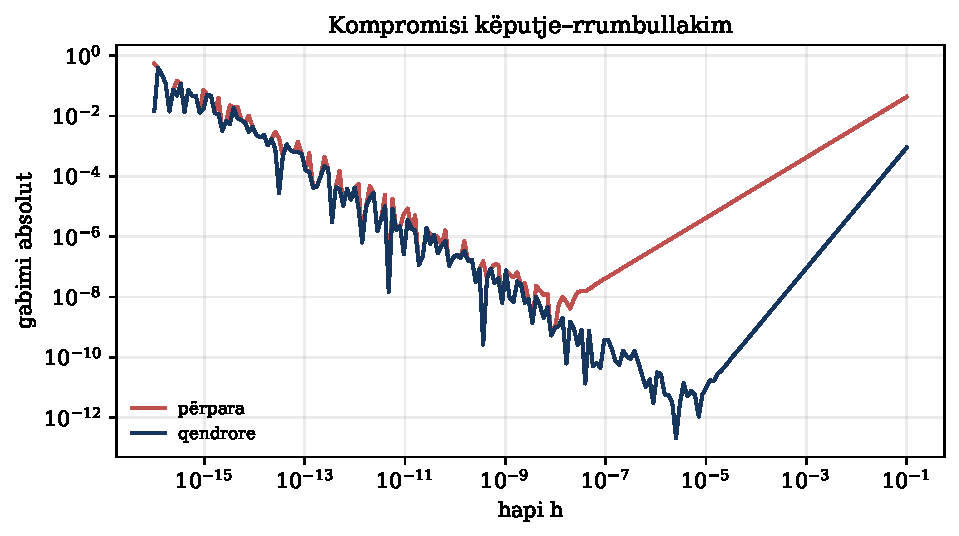
\includegraphics[width=.74\textwidth]{08_gabimi_derivimit.pdf}
\caption{Gabimi total ka formë U: këputja dominon për hapa të mëdhenj, rrumbullakimi për hapa tepër të vegjël.}
\end{figure}

\section{Kuadratura e përbërë}
Integrali ndahet në nënintervale. Rregulla e trapezit është
\begin{equation}
 T_n=h\left[\frac{f(a)+f(b)}2+\sum_{i=1}^{n-1}f(a+ih)\right],\qquad h=\frac{b-a}{n},
\end{equation}
me gabim global $\Oh(h^2)$. Rregulla e Simpsonit për $n$ çift është
\begin{equation}
 S_n=\frac h3\left[f_0+f_n+4\sum_{i\text{ tek}}f_i+2\sum_{i\text{ çift},\,i\ne0,n}f_i\right],
\end{equation}
me gabim global $\Oh(h^4)$ për funksione mjaft të lëmuara.

\begin{figure}[ht]
\centering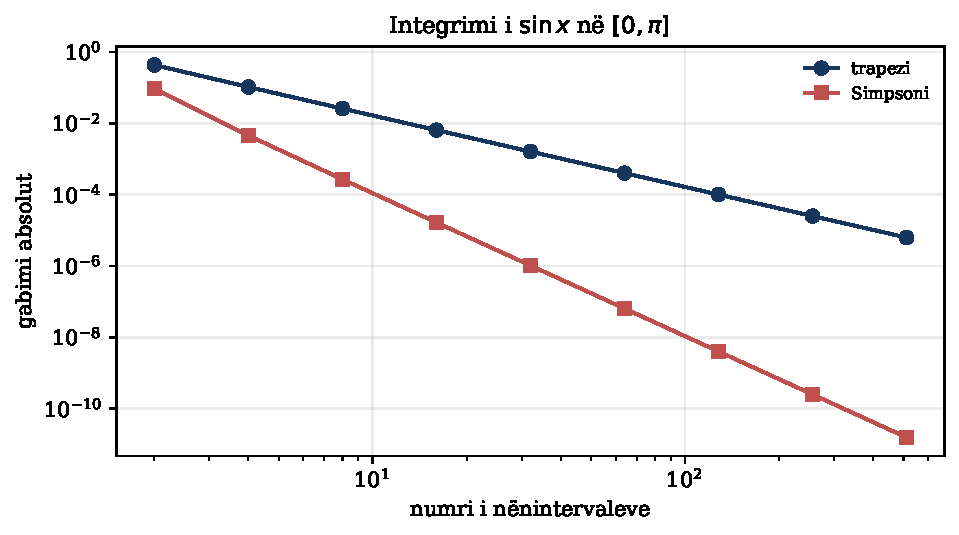
\includegraphics[width=.74\textwidth]{09_kuadratura_konvergjenca.pdf}
\caption{Konvergjenca e trapezit dhe Simpsonit për një integral me zgjidhje të njohur.}
\end{figure}

\section{Kuadratura e Gausit}
Rregulli me $n$ nyje
\begin{equation}
 \int_{-1}^{1}f(x)\dd x\approx\sum_{i=1}^{n}w_if(x_i)
\end{equation}
zgjedh nyjet si zerot e polinomit Legendre $P_n$. Ai integron saktë çdo polinom me gradë deri $2n-1$. Një transformim afin e çon intervalin $[a,b]$ në $[-1,1]$. Kuadratura Gauss është e fuqishme kur funksioni është i lëmuar dhe dimensioni i vogël.

\section{Integrale të papërshtatshme dhe shumëfishta}
Singularitetet e integrueshme trajtohen me ndryshim ndryshoreje ose ndarje të intervalit. Intervali i pafund mund të hartohet në interval të fundmë. Në $d$ përmasa, prodhimi tensorial i $n$ nyjeve kërkon $n^d$ vlerësime: mallkimi i dimensionalitetit. Kjo është pika ku metodat Monte Carlo bëhen konkurruese, sepse gabimi i tyre bazë varet nga numri i mostrave dhe jo drejtpërdrejt nga $d$.

\begin{shembull}[Perioda e lavjerrësit]
Për amplitudë $\theta_0$, perioda e saktë e modelit ideal është
\begin{equation}
 T=4\sqrt{\frac Lg}\int_0^{\pi/2}\frac{\dd\phi}{\sqrt{1-k^2\sin^2\phi}},\qquad k=\sin(\theta_0/2).
\end{equation}
Integrali eliptik mund të llogaritet me Simpson ose Gauss dhe të krahasohet me $T_0=2\pi\sqrt{L/g}$. Diferenca mat kufirin e përafrimit të këndit të vogël.
\end{shembull}

\begin{lidhje}
Laboratori llogarit periodën për disa amplituda, kryen studim konvergjence dhe ndan gabimin e kuadraturës nga gabimi i modelit $\sin\theta\approx\theta$.
\end{lidhje}

\section*{Pyetje kontrolli}
\begin{enumerate}
\item Pse derivati numerik nuk përmirësohet pafundësisht kur $h\to0$?
\item Çfarë kushti duhet për rendin e katërt të Simpsonit?
\item Pse prodhimi tensorial bëhet i papërshtatshëm në dimension të lartë?
\end{enumerate}
\section{Algoritmet e diferencimit dhe kuadraturës}
\subsection{Derivati qendror dhe studimi i hapit}
\begin{lstlisting}[language=Python,caption={Gabimi i derivatit qendror për një varg hapash.}]
import numpy as np

def derivat_qendror(f, x, h):
    return (f(x + h) - f(x - h)) / (2.0*h)

f = np.sin
x0 = 1.0
h = np.logspace(-16, -1, 200)
D = derivat_qendror(f, x0, h)
gabimi = np.abs(D - np.cos(x0))
h_opt = h[np.argmin(gabimi)]
print("h optimal empirik =", h_opt)
\end{lstlisting}
Grafiku $E(h)$ duhet të paraqitet në bosht log--log. Në zonën e këputjes pritet pjerrësi afërsisht 2; në zonën e rrumbullakimit gabimi rritet kur $h$ zvogëlohet.

\subsection{Rregulli i përbërë i Simpsonit}
\begin{lstlisting}[language=Python,caption={Integrimi Simpson me kontrollin e numrit çift të nënintervaleve.}]
def simpson(f, a, b, n):
    if n <= 0 or n % 2 != 0:
        raise ValueError("n duhet te jete numer pozitiv çift.")
    x = np.linspace(a, b, n + 1)
    y = f(x)
    h = (b - a) / n
    return h/3 * (y[0] + y[-1]
                  + 4*np.sum(y[1:-1:2])
                  + 2*np.sum(y[2:-2:2]))

for n in [4, 8, 16, 32, 64]:
    I = simpson(np.sin, 0.0, np.pi, n)
    print(n, I, abs(I - 2.0))
\end{lstlisting}

\subsection{Vlerësimi Runge i gabimit}
Nëse metoda ka rend $p$, dy llogaritje me $h$ dhe $h/2$ japin
\begin{equation}
 E_{h/2}\approx\frac{|A(h/2)-A(h)|}{2^p-1}.
\end{equation}
Ky vlerësim është i vlefshëm vetëm në regjimin asimptotik. Prandaj kontrollohet edhe raporti i gabimeve për tri hapa radhazi.

\begin{lstlisting}[language=Python]
def studim_konvergjence(llogarit, ns, p):
    v = np.array([llogarit(n) for n in ns])
    e_runge = np.abs(v[1:] - v[:-1]) / (2**p - 1)
    return v, e_runge
\end{lstlisting}

\subsection{Kuadratura e Gausit}
\begin{lstlisting}[language=Python,caption={Gauss--Legendre në një interval të përgjithshëm.}]
from numpy.polynomial.legendre import leggauss

def gauss_legendre(f, a, b, n):
    xi, w = leggauss(n)
    x = 0.5*(b-a)*xi + 0.5*(a+b)
    return 0.5*(b-a) * np.sum(w * f(x))
\end{lstlisting}
Në notebook krahasohen numri i vlerësimeve të funksionit, gabimi dhe koha e ekzekutimit. Kjo e lidh kuadraturën klasike me motivimin për Monte Carlo në dimension të lartë.

Formulat dhe emërtimet shqip të diferencimit e integrimit numerik mbështeten te \cite{hanelli,hoxha,datja}; interpretimi fizik dhe krahasimi me Monte Carlo plotësohen nga \cite{newman,press}.

\subsection{Nxjerrja sistematike e formulave të diferencimit}
Nga zhvillimet Taylor
\begin{align}
 f(x+h)&=f(x)+hf'(x)+\frac{h^2}{2}f''(x)+\frac{h^3}{6}f'''(x)+\Oh(h^4),\\
 f(x-h)&=f(x)-hf'(x)+\frac{h^2}{2}f''(x)-\frac{h^3}{6}f'''(x)+\Oh(h^4)
\end{align}
dalin dy kombinime të rëndësishme. Zbritja e barazimeve anulon termat çift dhe jep
\begin{equation}
 f'(x)=\frac{f(x+h)-f(x-h)}{2h}-\frac{h^2}{6}f'''(x)+\Oh(h^4),
\end{equation}
pra diferenca qendrore ka gabim të këputjes $\Oh(h^2)$. Mbledhja anulon termat tek dhe jep
\begin{equation}
 f''(x)=\frac{f(x+h)-2f(x)+f(x-h)}{h^2}-\frac{h^2}{12}f^{(4)}(x)+\Oh(h^4).
\end{equation}
Koeficientët e formulave me më shumë pika gjenden duke kërkuar që kombinimi linear të riprodhojë saktë monomet $1,x,x^2,\ldots$ deri në gradën e dëshiruar.

Gabimi i rrumbullakimit në diferencën e parë rritet afërsisht si $u|f|/h$, ndërsa gabimi i këputjes për diferencën qendrore ulet si $C h^2$. Modeli
\begin{equation}
 E(h)\simeq C_1h^2+C_2\frac{u}{h}
\end{equation}
ka minimum për $h_{\mathrm{opt}}\sim u^{1/3}$. Kjo shpjegon formën në U të grafikut të gabimit: zvogëlimi i pakufizuar i hapit nuk rrit saktësinë.

\subsection{Rregulla e trapezit dhe termi i gabimit}
Në intervalin $[a,b]$, polinomi linear interpolues është
\begin{equation}
 p_1(x)=f(a)\frac{b-x}{b-a}+f(b)\frac{x-a}{b-a}.
\end{equation}
Integrimi i tij jep
\begin{equation}
 T_1=\frac{b-a}{2}[f(a)+f(b)].
\end{equation}
Nga mbetja e interpolimit ose nga Taylor-i rreth mesit merret
\begin{equation}
 \int_a^b f(x)\dd x-T_1=-\frac{(b-a)^3}{12}f''(\xi).
\end{equation}
Për $n$ nënintervale me hap $h=(b-a)/n$, mbledhja e gabimeve lokale jep gabim global
\begin{equation}
 E_T=-\frac{b-a}{12}h^2 f''(\xi),
\end{equation}
pra rregulla e përbërë është e rendit të dytë.

\subsection{Rregulla e Simpsonit}
Mbi dy nënintervale, integrohet polinomi kuadratik që kalon në $x_0$, $x_1=x_0+h$ dhe $x_2=x_0+2h$:
\begin{equation}
 S_2=\frac{h}{3}[f(x_0)+4f(x_1)+f(x_2)].
\end{equation}
Edhe pse interpoluesi ka gradë dy, simetria e bën rregullën të saktë edhe për polinomet kubike. Gabimi lokal është
\begin{equation}
 -\frac{h^5}{90}f^{(4)}(\xi),
\end{equation}
ndërsa përbërja në një interval të fiksuar jep gabim global $\Oh(h^4)$. Numri i nënintervaleve duhet të jetë çift. Një kod i mirë e verifikon këtë parakusht, në vend që të prodhojë në heshtje një rezultat të pakuptimtë.

\subsection{Kuadratura e Gausit}
Kërkohen nyje $x_i$ dhe pesha $w_i$ të tilla që
\begin{equation}
 \int_{-1}^{1}f(x)\dd x\approx\sum_{i=1}^{n}w_if(x_i)
\end{equation}
të jetë e saktë për gradën më të lartë të mundshme. Me $2n$ parametra përcaktohen momentet deri në gradën $2n-1$. Nyjet optimale janë rrënjët e polinomit Legendre $P_n$. Për $n=2$, simetria kërkon nyje $\pm a$ dhe pesha të barabarta $w$; saktësia për $1$ dhe $x^2$ jep $2w=2$ dhe $2wa^2=2/3$, prandaj $w=1$ dhe $a=1/\sqrt3$.

Për intervalin $[a,b]$ përdoret transformimi
\begin{equation}
 x=\frac{a+b}{2}+\frac{b-a}{2}\xi,qquad
 \dd x=\frac{b-a}{2}\dd\xi.
\end{equation}
Avantazhi është saktësia e lartë me pak vlerësime; kufizimi është se nyjet nuk janë të futura natyrshëm, prandaj kontrolli adaptiv kërkon çifte rregullash ose nënndarje.

\begin{lstlisting}[language=Python,caption={Simpson i përbërë me kontroll të dyfishimit të rrjetit.}]
import numpy as np

def simpson(f, a, b, n):
    if n <= 0 or n % 2:
        raise ValueError("n duhet të jetë numër pozitiv çift.")
    x = np.linspace(a, b, n + 1)
    h = (b - a) / n
    return (h / 3.0) * (f(x[0]) + f(x[-1])
           + 4.0*np.sum(f(x[1:-1:2]))
           + 2.0*np.sum(f(x[2:-1:2])))

def kontroll_simpson(f, a, b, n):
    I_h = simpson(f, a, b, n)
    I_h2 = simpson(f, a, b, 2*n)
    gabimi = abs(I_h2 - I_h) / (2.0**4 - 1.0)
    return I_h2, gabimi
\end{lstlisting}

\subsection{Përmbledhje dhe ushtrime}
Derivimi numerik është intrinsikisht më i ndjeshëm ndaj zhurmës, ndërsa integrimi ka efekt mesatarizues. Rendi formal duhet konfirmuar me një studim rrjeti dhe jo vetëm cituar.
\begin{enumerate}
\item Nxirrni formulën qendrore me pesë pika për $f'(x)$ dhe termin kryesor të gabimit.
\item Vërtetoni saktësinë kubike të Simpsonit duke integruar monomet $1,x,x^2,x^3$.
\item Ndërtoni Gauss--Legendre me tri pika nga momentet dhe simetria.
\item Llogaritni periodën e lavjerrësit si integral dhe krahasoni Simpsonin me Gauss-in.
\end{enumerate}

\subsection{Kuadratura adaptive dhe vlerësimi lokal i gabimit}
Një rrjet uniform harxhon pika në rajone ku funksioni është i lëmuar dhe mund të mos zgjidhë rajone me ndryshim të shpejtë. Kuadratura adaptive e ndan intervalin aty ku gabimi i vlerësuar është i madh. Për Simpsonin, le të jenë $S(a,b)$ vlerësimi në të gjithë intervalin dhe
\begin{equation}
 S_2=S(a,m)+S(m,b),\qquad m=\frac{a+b}{2}.
\end{equation}
Meqë gabimi kryesor shkallëzohet si $h^4$ globalisht, vlerësimi i Richardson-it është
\begin{equation}
 E\approx\frac{S_2-S(a,b)}{2^4-1}.
\end{equation}
Nëse $|E|$ është nën tolerancën lokale, pranohet $S_2+E$; përndryshe të dy gjysmat ndahen rekursivisht. Toleranca globale ndahet ndërmjet intervaleve, për shembull përgjysmohet në çdo degë. Duhet vendosur thellësi maksimale për të shmangur rekursion të pafundëm pranë singulariteteve ose zhurmës.

Vlerësimi mund të dështojë kur dy rregullat japin rastësisht të njëjtin rezultat, kur funksioni ka një kulm shumë të ngushtë që nuk kapet nga pikat ose kur ka ndërprerje. Një algoritëm profesional kombinon rregulla të futura Gauss--Kronrod, zbulim të sjelljes së keqe dhe raport të statusit, jo vetëm një numër.

\subsubsection{Integralet e papërshtatshme}
Për një kufi të pafundëm, transformimi
\begin{equation}
 x=\frac{t}{1-t},\qquad \dd x=\frac{\dd t}{(1-t)^2},\qquad 0\le t<1,
\end{equation}
e kthen $[0,\infty)$ në $[0,1)$. Transformimi duhet zgjedhur sipas shuarjes së integrandit; Jakobi mund të krijojë një funksion të vështirë pranë $t=1$. Një alternativë është prerja në $R$ dhe kufizimi analitik i bishtit.

Për singularitetin integrueshëm $x^{-1/2}$ në zero, zëvendësimi $x=t^2$ jep
\begin{equation}
 \int_0^1\frac{g(x)}{\sqrt x}\dd x
 =2\int_0^1g(t^2)\dd t,
\end{equation}
që është i rregullt nëse $g$ është i lëmuar. Njohja e strukturës analitike është më efikase se zvogëlimi brutal i hapit.

\subsubsection{Integralet shumëpërmasore}
Rregulli tensorial me $n$ pika për bosht kërkon $n^d$ vlerësime në $d$ përmasa. Kjo është mallkimi i dimensionalitetit. Për dimensione të ulëta dhe integrandë të lëmuar, kuadratura tensoriale ose rrjetet e rralla mund të jenë shumë të sakta. Për dimensione të larta, Monte Carlo me gabim $N^{-1/2}$ bëhet konkurrues sepse eksponenti nuk varet shprehimisht nga $d$.

Megjithatë, dimensioni ndikon përmes variancës dhe gjeometrisë. Nëse rajoni $D$ zë një pjesë jashtëzakonisht të vogël të kutisë kufizuese, metoda hit-or-miss ka variancë të madhe. Një parametrizim që gjeneron pika drejtpërdrejt në $D$ është shumë më efikas. Për një disk, përdorimi i $r=R\sqrt U$ dhe $\theta=2\pi V$ prodhon shpërndarje uniforme në sipërfaqe; zgjedhja $r=RU$ do të grumbullonte pika pranë qendrës.

\subsubsection{Verifikimi me funksione prove}
Një rutinë integrimi testohet me polinome të gradës së saktësisë, funksione periodike, kulme të ngushta dhe raste me zgjidhje të njohur. Rendi matet duke vizatuar gabimin ndaj hapit në shkallë log--log. Pjerrësia duhet të jetë pranë rendit teorik vetëm para se rrumbullakimi të dominojë. Raporti duhet të përmbajë numrin e vlerësimeve të funksionit; dy metoda me të njëjtin gabim mund të kenë kosto shumë të ndryshme.


\chapter{Ekuacionet diferenciale dhe dinamika numerike}
\begin{qellime}
Studenti zbaton Eulerin, Runge--Kutta dhe skemat me shumë hapa; analizon gabimin lokal, global dhe stabilitetin; simulon rënien e lirë, lavjerrësin dhe problemin e dy trupave; dallon probleme fillestare e kufitare.
\end{qellime}

\section{Problemi i vlerës fillestare}
Për
\begin{equation}
 \dot{\vect y}=\vect f(t,\vect y),\qquad \vect y(t_0)=\vect y_0,
\end{equation}
metoda e Eulerit është
\begin{equation}
 \vect y_{n+1}=\vect y_n+h\vect f(t_n,\vect y_n).
\end{equation}
Gabimi lokal është $\Oh(h^2)$ dhe gabimi global $\Oh(h)$. Euler-i është i dobishëm pedagogjikisht, por rrallë është zgjedhja përfundimtare.

Metoda e mesit dhe Heun janë të rendit të dytë. Metoda klasike RK4 përdor katër pjerrësi,
\begin{align}
 \vect k_1&=\vect f(t_n,\vect y_n),\\
 \vect k_2&=\vect f(t_n+h/2,\vect y_n+h\vect k_1/2),\\
 \vect k_3&=\vect f(t_n+h/2,\vect y_n+h\vect k_2/2),\\
 \vect k_4&=\vect f(t_n+h,\vect y_n+h\vect k_3),\\
 \vect y_{n+1}&=\vect y_n+\frac h6(\vect k_1+2\vect k_2+2\vect k_3+\vect k_4).
\end{align}
Çiftet e futura Runge--Kutta me dy rende japin vlerësim të gabimit dhe hap adaptiv.

\section{Stabiliteti}
Për ekuacionin provë $y'=\lambda y$, Euler-i jep $y_{n+1}=(1+h\lambda)y_n$. Stabiliteti kërkon $|1+h\lambda|<1$. Një metodë mund të ketë rend të lartë dhe përsëri të jetë e papërshtatshme për problem të ngurtë. Ngurtësia shfaqet kur shkallë kohore shumë të ndryshme imponojnë hap shumë të vogël për metoda eksplicite.

\section{Metodat me shumë hapa}
Adams--Bashforth përdor pjerrësi të mëparshme, për shembull
\begin{equation}
 y_{n+1}=y_n+\frac h2(3f_n-f_{n-1}).
\end{equation}
Këto metoda janë ekonomike pas nisjes, por kërkojnë histori dhe kujdes kur ndryshon hapi. Metodat implícite Adams--Moulton dhe BDF kanë zona stabiliteti më të favorshme për probleme të ngurta.

\section{Dinamikë Hamiltoniane}
Në mekanikë, ruajtja afatgjatë e strukturës mund të jetë më e rëndësishme se gabimi lokal minimal. Skema leapfrog/Verlet është simplektike:
\begin{align}
 \vect v_{n+1/2}&=\vect v_n+\frac h2\vect a(\vect r_n),\\
 \vect r_{n+1}&=\vect r_n+h\vect v_{n+1/2},\\
 \vect v_{n+1}&=\vect v_{n+1/2}+\frac h2\vect a(\vect r_{n+1}).
\end{align}
Ajo është e kthyeshme në kohë dhe mban energjinë të kufizuar rreth vlerës së saktë, në vend që të krijojë drift sistematik.

\begin{figure}[ht]
\centering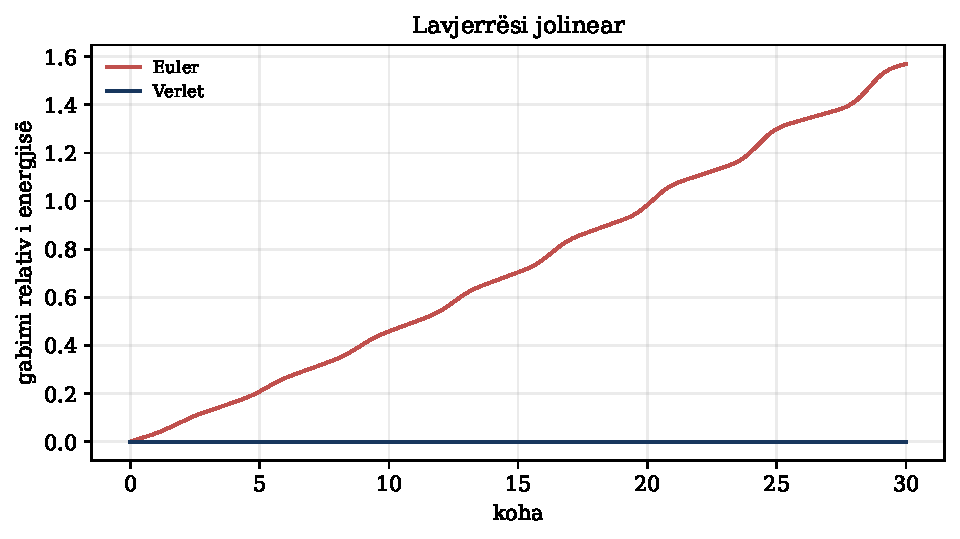
\includegraphics[width=.74\textwidth]{10_energjia_lavjerresit.pdf}
\caption{Euler-i krijon drift energjie, ndërsa Verlet ruan më mirë strukturën afatgjatë.}
\end{figure}

\section{Shembuj fizikë}
\subsection{Rënia në ajër}
Për bosht pozitiv lart,
\begin{equation}
 \dot y=v,\qquad m\dot v=-mg-c_1v-c_2v|v|.
\end{equation}
Modeli lejon krahasimin e rezistencës lineare dhe kuadratike, shpejtësisë terminale dhe ndjeshmërisë ndaj parametrave.

\subsection{Lavjerrësi jolinear}
\begin{equation}
 \ddot\theta+\gamma\dot\theta+\frac gL\sin\theta=A\cos\Omega t.
\end{equation}
Pa forcim dhe fërkim, energjia ruhet. Me forcim mund të shfaqen rezonancë, shumëstabilitet dhe kaos; hapi duhet kontrolluar ndaj periodës më të shkurtër.

\subsection{Problemi i dy trupave}
Në njësi të shkallëzuara,
\begin{equation}
 \ddot{\vect r}=-\mu\frac{\vect r}{r^3}.
\end{equation}
Kontrollet janë energjia, momenti këndor dhe ligji i tretë i Keplerit. Një orbitë që duket e mbyllur për pak perioda mund të ketë drift të ngadalshëm numerik.

\begin{figure}[ht]
\centering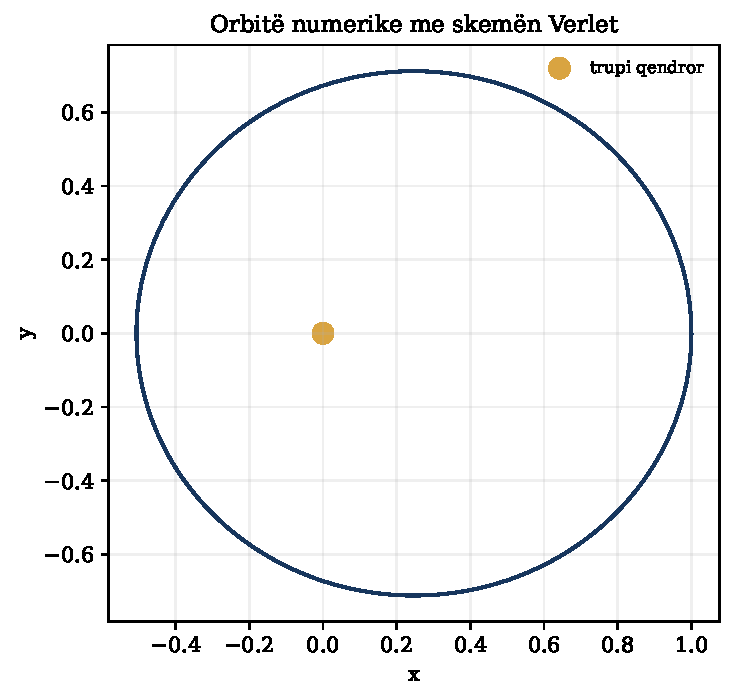
\includegraphics[width=.60\textwidth]{11_orbita_dy_trupave.pdf}
\caption{Orbitë e integruar me skemë simplektike.}
\end{figure}

\section{Problemet e vlerave kufitare}
Në një problem kufitar, kushtet jepen në skaje të ndryshme. Metoda e qitjes e kthen problemin në një kërkim të kushtit fillestar që plotëson skajin tjetër. Diferencat e fundme e kthejnë ekuacionin në sistem algjebrik. Qitja mund të jetë e ndjeshme; formulimi matricor është shpesh më robust.

\begin{lidhje}
Laboratori krahason Euler, RK4 dhe Verlet për rënien, lavjerrësin dhe orbitën. Për çdo metodë vizatohen gabimi, energjia dhe kostoja kundrejt hapit.
\end{lidhje}

\section*{Pyetje kontrolli}
\begin{enumerate}
\item Dalloni rendin nga stabiliteti.
\item Pse një metodë simplektike mund të jetë më e mirë për orbita afatgjata?
\item Si verifikohet numerikisht një integrues orbital?
\end{enumerate}
\section{Integruesit kohorë në Python}
\subsection{Euler dhe Runge--Kutta i rendit të katërt}
\begin{lstlisting}[language=Python,caption={Dy integrues të përgjithshëm për sisteme ODE.}]
def euler(f, t, y0):
    y = np.empty((len(t), len(np.atleast_1d(y0))), float)
    y[0] = y0
    for n, h in enumerate(np.diff(t)):
        y[n+1] = y[n] + h*f(t[n], y[n])
    return y

def rk4(f, t, y0):
    y = np.empty((len(t), len(np.atleast_1d(y0))), float)
    y[0] = y0
    for n, h in enumerate(np.diff(t)):
        k1 = f(t[n], y[n])
        k2 = f(t[n]+h/2, y[n]+h*k1/2)
        k3 = f(t[n]+h/2, y[n]+h*k2/2)
        k4 = f(t[n]+h, y[n]+h*k3)
        y[n+1] = y[n] + h*(k1+2*k2+2*k3+k4)/6
    return y
\end{lstlisting}

\subsection{Modeli i lavjerrësit}
\begin{lstlisting}[language=Python]
def lavjerresi(t, y, g=9.81, L=1.0, gamma=0.0):
    theta, omega = y
    return np.array([omega, -g/L*np.sin(theta) - gamma*omega])

def energjia(y, g=9.81, L=1.0):
    theta, omega = y.T
    return 0.5*(L*omega)**2 + g*L*(1-np.cos(theta))
\end{lstlisting}
Për rastin pa fërkim, drift-i i energjisë mat cilësinë afatgjatë. Për rastin me fërkim, energjia duhet të bjerë; ruajtja nuk është më kontrolli i duhur.

\subsection{Velocity Verlet për gravitetin}
\begin{lstlisting}[language=Python,caption={Skema simplektike për orbitën.}]
def verlet_orbite(r0, v0, dt, n, mu=1.0):
    r = np.empty((n, 2)); v = np.empty((n, 2))
    r[0], v[0] = r0, v0
    def a(q):
        return -mu*q/np.linalg.norm(q)**3
    for k in range(n-1):
        v_half = v[k] + 0.5*dt*a(r[k])
        r[k+1] = r[k] + dt*v_half
        v[k+1] = v_half + 0.5*dt*a(r[k+1])
    return r, v
\end{lstlisting}

\subsection{Protokolli i verifikimit}
\begin{enumerate}
\item Euler-i testohet te $y'=\lambda y$, ku zgjidhja njihet.
\item RK4 testohet me përgjysmim hapi dhe pritet faktor gabimi afërsisht $2^4$.
\item Për orbitën kontrollohen energjia dhe momenti këndor.
\item Për lavjerrësin e këndit të vogël krahasohet perioda me $2\pi\sqrt{L/g}$.
\item Koha dhe memoria raportohen bashkë me gabimin.
\end{enumerate}

\begin{kujdes}
Në terminologjinë numerike shqipe përdoren \emph{metodë e shtjelluar} dhe \emph{metodë e pashtjelluar} për explicit dhe implicit. Në tekst jepen edhe termat ndërkombëtarë kur ndihmojnë studentin të lexojë dokumentacionin e bibliotekave.
\end{kujdes}

Për terminologjinë \emph{problem i vlerës fillestare}, \emph{gabim lokal}, \emph{gabim global}, \emph{metodë e shtjelluar} dhe \emph{qëndrueshmëri} janë përdorur gjerësisht burimet shqip \cite{dishmema,hanelli,hoxha,datja,dishmemaArticle}.

\subsection{Gabimi lokal dhe global i Eulerit}
Për problemin $\vect y'=\vect f(t,\vect y)$, Taylor-i i zgjidhjes së saktë është
\begin{equation}
 \vect y(t_n+h)=\vect y(t_n)+h\vect f(t_n,\vect y(t_n))
 +\frac{h^2}{2}\vect y''(\xi_n).
\end{equation}
Euler-i heq termin e fundit; defekti lokal është $\Oh(h^2)$. Nëse $\vect f$ është Lipschitz në $\vect y$ me konstante $L$, gabimet plotësojnë afërsisht
\begin{equation}
 \|\vect e_{n+1}\|\le(1+hL)\|\vect e_n\|+Ch^2.
\end{equation}
Pas $N=T/h$ hapash dhe përdorimit të pabarazisë diskrete të Grönwall-it merret $\|\vect e_N\|\le C_T h$: rendi global është një më i ulët se rendi i defektit lokal.

\subsection{Qëndrueshmëria absolute}
Ekuacioni provë $y'=\lambda y$ ndan metodën nga problemi. Euler-i jep
\begin{equation}
 y_{n+1}=(1+h\lambda)y_n.
\end{equation}
Për një zgjidhje fizike që shuhet, $\Re\lambda<0$, kërkohet $|1+h\lambda|<1$. Bashkësia $\{z:|1+z|<1\}$ është rajoni i qëndrueshmërisë absolute. Për $\lambda<0$ real, kushti bëhet $0<h<2/|\lambda|$. Një hap mund të jetë mjaft i vogël për saktësi dhe përsëri i papërshtatshëm për qëndrueshmëri, ose anasjelltas.

Problemet e shtyllura përmbajnë shkallë kohore shumë të ndryshme. Metodat eksplicite detyrohen të ndjekin shkallën më të shpejtë edhe kur interesi fizik është te evolucioni i ngadaltë. Euler-i i prapëm ka faktor $1/(1-h\lambda)$ dhe është i qëndrueshëm për të gjithë gjysmëplanin $\Re(h\lambda)<0$, por kërkon zgjidhje algjebrike në çdo hap.

\subsection{Runge--Kutta i rendit të katërt}
Metodat Runge--Kutta përputhin zhvillimin Taylor pa llogaritur derivate të larta të $\vect f$. Skema klasike është
\begin{align}
 \vect k_1&=\vect f(t_n,\vect y_n),\\
 \vect k_2&=\vect f(t_n+h/2,\vect y_n+h\vect k_1/2),\\
 \vect k_3&=\vect f(t_n+h/2,\vect y_n+h\vect k_2/2),\\
 \vect k_4&=\vect f(t_n+h,\vect y_n+h\vect k_3),\\
 \vect y_{n+1}&=\vect y_n+\frac{h}{6}(\vect k_1+2\vect k_2+2\vect k_3+\vect k_4).
\end{align}
Koeficientët plotësojnë kushtet e rendit që barazojnë zhvillimin e skemës me Taylor-in deri në $h^4$. Gabimi lokal është $\Oh(h^5)$ dhe globali $\Oh(h^4)$. Katër vlerësime të funksionit kushtojnë më shumë se Euler-i, por për një tolerancë të dhënë zakonisht lejojnë hapa shumë më të mëdhenj.

\subsection{Metodat me shumë hapa}
Integrimi i identitetit
\begin{equation}
 \vect y(t_{n+1})=\vect y(t_n)+\int_{t_n}^{t_{n+1}}\vect f(t,\vect y(t))\dd t
\end{equation}
dhe interpolimi i $\vect f$ në pika të mëparshme jep Adams--Bashforth. Për dy hapa,
\begin{equation}
 \vect y_{n+1}=\vect y_n+h\left(\frac32\vect f_n-\frac12\vect f_{n-1}\right).
\end{equation}
Metoda kursen vlerësime të funksionit, por nuk nis vetë: nevojitet një metodë njëhapëshe për gjendjet fillestare. Stabiliteti dhe rrënjët e polinomit karakteristik duhet të kontrollohen; një formulë me rend formal të lartë mund të jetë zero-e-paqëndrueshme.

\subsection{Leapfrog, Verlet dhe dinamika Hamiltoniane}
Për $\ddot q=a(q)$, velocity Verlet shkruhet
\begin{align}
 v_{n+1/2}&=v_n+\frac h2a(q_n),\\
 q_{n+1}&=q_n+hv_{n+1/2},\\
 v_{n+1}&=v_{n+1/2}+\frac h2a(q_{n+1}).
\end{align}
Skema është e kthyeshme në kohë dhe simplektike. Ajo nuk e ruan energjinë pikë për pikë, por ruan një Hamiltonian të modifikuar pranë atij të vërtetë; prandaj gabimi i energjisë lëkundet pa drift sistematik për kohë të gjata. Kjo është arsyeja strukturore pse Verlet-i mund të jetë më i mirë se një metodë me rend lokal më të lartë për orbita afatgjata.

\subsection{Problemet kufitare}
Për $y''=f(x,y,y')$ me $y(a)=\alpha$, $y(b)=\beta$, metoda e qitjes e zëvendëson pjerrësinë e panjohur $s=y'(a)$ me parametër. Integrohet problemi fillestar dhe zgjidhet ekuacioni skalar
\begin{equation}
 \Phi(s)=y(b;s)-\beta=0.
\end{equation}
Qitja është intuitive, por mund të jetë e keqkushtëzuar. Diferencat e fundme ndërtojnë një sistem algjebrik për të gjitha nyjet dhe janë më të përshtatshme kur zgjidhja rritet ose shuhet shumë shpejt.

\subsection{Përmbledhje dhe ushtrime}
Zgjedhja e integruesit varet jo vetëm nga rendi, por nga stabiliteti, struktura e sistemit dhe horizonti kohor.
\begin{enumerate}
\item Nxirrni rajonin e qëndrueshmërisë së Eulerit të përmirësuar.
\item Verifikoni rendet e Eulerit dhe RK4 me metodën e përgjysmimit të hapit.
\item Krahasoni RK4 dhe Verlet për orbitën e Keplerit duke matur energjinë dhe momentin këndor.
\item Zgjidhni një problem kufitar me qitje dhe me diferenca të fundme; diskutoni kushtëzimin.
\end{enumerate}

\subsection{Lavjerrësi jolinear dhe perioda e varur nga amplituda}
Ekuacioni pa fërkim është
\begin{equation}
 \ddot\theta+\frac{g}{L}\sin\theta=0.
\end{equation}
Linearizimi $\sin\theta\simeq\theta$ jep periodën $T_0=2\pi\sqrt{L/g}$, por modeli linear humbet varësinë nga amplituda. Nga ruajtja e energjisë,
\begin{equation}
 \frac12L^2\dot\theta^2+gL(1-\cos\theta)
 =gL(1-\cos\theta_0),
\end{equation}
merret perioda
\begin{equation}
 T=4\sqrt{\frac{L}{g}}
 \int_0^{\pi/2}\frac{\dd\phi}
 {\sqrt{1-k^2\sin^2\phi}},
 \qquad k=\sin\frac{\theta_0}{2}.
\end{equation}
Ky integral eliptik mund të llogaritet me kuadraturë dhe të krahasohet me periodën e nxjerrë nga integrimi kohor. Për amplituda të vogla,
\begin{equation}
 \frac{T}{T_0}=1+\frac{\theta_0^2}{16}
 +\frac{11\theta_0^4}{3072}+\cdots.
\end{equation}
Krahasimi i tri rrugëve --- seria, kuadratura dhe ODE-ja --- është verifikim i fuqishëm ndërmetodik.

Perioda numerike nga trajektorja matet me kalime në zero ose me kulme. Interpolimi ndërmjet dy hapave zvogëlon gabimin e kuantizimit kohor. Për integrim afatgjatë, monitorohet energjia. Një metodë jo simplektike mund të japë periodë të mirë për disa cikle dhe pastaj të krijojë drift që ndryshon artificialisht amplitudën.

\subsubsection{Problemi i dy trupave dhe reduktimi në një trup}
Për masa $m_1,m_2$ me pozicione $\vect r_1,\vect r_2$, forcat janë të barabarta e të kundërta. Qendra e masës
\begin{equation}
 \vect R=\frac{m_1\vect r_1+m_2\vect r_2}{m_1+m_2}
\end{equation}
lëviz në mënyrë uniforme, ndërsa koordinata relative $\vect r=\vect r_1-\vect r_2$ plotëson
\begin{equation}
 \mu\ddot{\vect r}=-\frac{Gm_1m_2}{r^3}\vect r,
 \qquad \mu=\frac{m_1m_2}{m_1+m_2}.
\end{equation}
Pas pjesëtimit me $\mu$ merret $\ddot{\vect r}=-G(m_1+m_2)\vect r/r^3$. Invariantet janë energjia
\begin{equation}
 E=\frac12\mu|\dot{\vect r}|^2-\frac{Gm_1m_2}{r}
\end{equation}
dhe momenti këndor $\vect L=\mu\vect r\times\dot{\vect r}$. Për orbitë të lidhur me gjysmëbosht të madh $a$,
\begin{equation}
 T^2=\frac{4\pi^2}{G(m_1+m_2)}a^3.
\end{equation}
Një laborator i plotë nxjerr periodën nga simulimi për disa $a$, përshtat pjerrësinë në shkallë logaritmike dhe kontrollon konstanten fizike, jo vetëm eksponentin $3/2$.

\subsubsection{Gabimi në ngjarje dhe hapa adaptivë}
Shumë probleme kërkojnë kohën e një ngjarjeje: goditja e tokës, kalimi në periapsis ose arritja e një pragu. Nëse ngjarja ndodh ndërmjet $t_n$ dhe $t_{n+1}$, kthimi i thjeshtë i $t_{n+1}$ ka gabim të rendit $h$. Duhet interpoluar funksioni i ngjarjes $g(t,y)$ dhe zgjidhur $g=0$ brenda hapit. Bibliotekat ODE e bëjnë këtë me interpolues të dendur, por përdoruesi duhet të përcaktojë drejtimin e kalimit dhe nëse integrimi ndalet.

Kontrolli adaptiv përdor dy vlerësime me rende të ndryshme ose step-doubling. Nëse gabimi lokal i vlerësuar është $e$, hapi i ri zgjidhet afërsisht
\begin{equation}
 h_{\mathrm{ri}}=s h\left(\frac{\mathrm{tol}}{e}\right)^{1/(p+1)},
\end{equation}
me faktor sigurie $s<1$. Toleranca absolute mbron komponentët pranë zeros; toleranca relative shkallëzon komponentët e mëdhenj. Në sisteme me njësi të ndryshme nevojiten toleranca komponentore ose nondimensionalizim.


\chapter{Diferencat e fundme dhe simulimi i valëve}
\begin{qellime}
Studenti diskretizon derivatet hapësinore; ndërton skemën për ekuacionin e valës; zbaton kushte fillestare e kufitare; analizon kushtin CFL, dispersimin dhe reflektimin; interpreton valët bredhëse e të qëndrueshme.
\end{qellime}

\section{Nga PDE te rrjeti}
Në rrjetin $x_j=j\Delta x$, $t^n=n\Delta t$, fusha përfaqësohet nga $u_j^n\approx u(x_j,t^n)$. Për ekuacionin e valës
\begin{equation}
 \frac{\partial^2u}{\partial t^2}=c^2\frac{\partial^2u}{\partial x^2},
\end{equation}
diferencat qendrore japin
\begin{equation}
 u_j^{n+1}=2u_j^n-u_j^{n-1}+r^2(u_{j+1}^n-2u_j^n+u_{j-1}^n),
 \qquad r=\frac{c\Delta t}{\Delta x}.
\end{equation}
Skema është eksplicite dhe e rendit të dytë në kohë e hapësirë.

\section{Kushtet fillestare dhe kufitare}
Nevojiten zhvendosja $u(x,0)$ dhe shpejtësia $u_t(x,0)$. Hapi i parë ndërtohet me zhvillim Taylor. Skaji i fiksuar përdor Dirichlet, $u=0$; skaji i lirë përdor Neumann, $u_x=0$; një skaj thithës synon të minimizojë valën e reflektuar.

\begin{figure}[ht]
\centering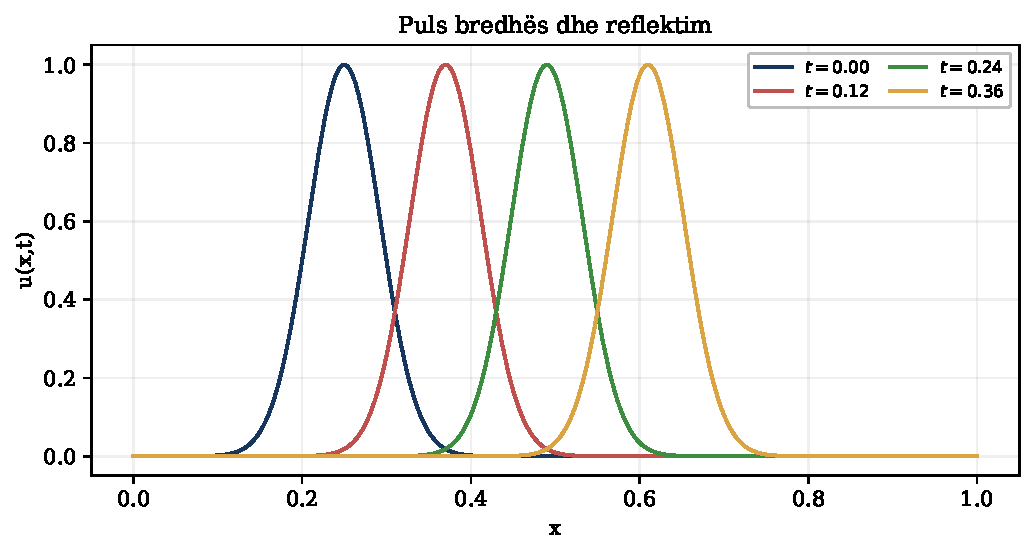
\includegraphics[width=.82\textwidth]{12_vala_bredhese.pdf}
\caption{Evolucioni i një pulsi bredhës dhe përafrimi te kufiri reflektues.}
\end{figure}

\section{Stabiliteti CFL}
Analiza von Neumann zëvendëson $u_j^n$ me një mod Fourier $G^n e^{ikj\Delta x}$. Për skemën standarde në një përmasë merret kushti
\begin{equation}
 r=\frac{c\Delta t}{\Delta x}\le1.
\end{equation}
Ky kusht ka interpretim kauzal: domeni numerik i varësisë duhet të përmbajë domenin fizik. Shkelja e tij prodhon rritje eksponenciale të gabimeve.

\section{Dispersimi numerik}
Edhe kur skema është stabile, frekuenca numerike nuk përputhet saktësisht me $\omega=ck$. Për rrjetin hapësinor,
\begin{equation}
 k_{\mathrm{eff}}=\frac{2}{\Delta x}\sin\frac{k\Delta x}{2}.
\end{equation}
Modet me gjatësi vale pranë $2\Delta x$ përhapen gabim. Një rregull praktik kërkon shumë pika për gjatësi vale, jo vetëm dy.

\begin{figure}[ht]
\centering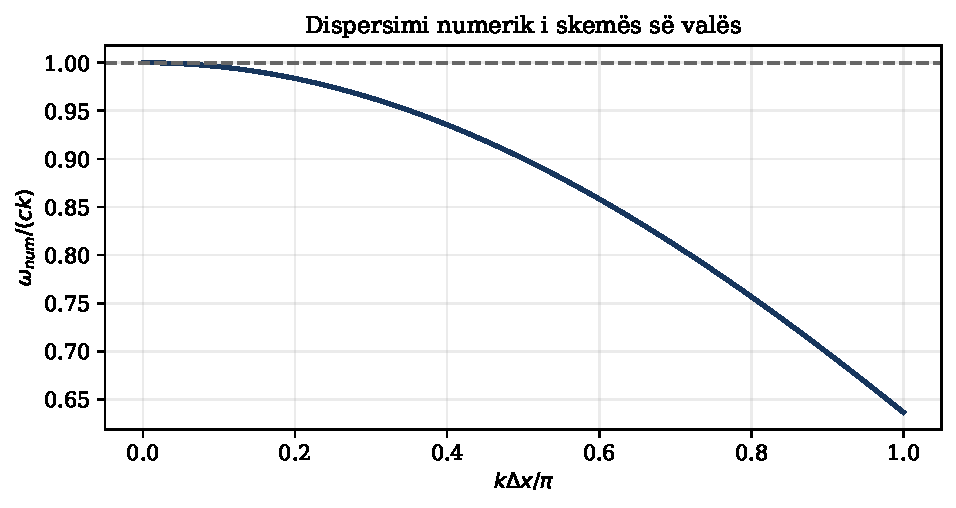
\includegraphics[width=.73\textwidth]{13_dispersimi_numerik.pdf}
\caption{Shpejtësia fazore numerike zvogëlohet për numra valorë të lartë.}
\end{figure}

\section{Valët e qëndrueshme}
Për skaje të fiksuara, zgjidhjet modale janë
\begin{equation}
 u_n(x,t)=A_n\sin\frac{n\pi x}{L}\cos(\omega_nt+\phi_n),\qquad
 \omega_n=\frac{n\pi c}{L}.
\end{equation}
Simulimi mund të nxjerrë spektrin përmes transformimit Fourier të sinjalit në një pikë. Krahasimi me $\omega_n$ verifikon rrjetin dhe kushtet kufitare.

\section{Reflektimi nga plazma}
Në një plazmë të ftohtë pa fushë magnetike,
\begin{equation}
 \varepsilon_r(\omega)=1-\frac{\omega_p^2}{\omega^2},\qquad
 \omega_p=\sqrt{\frac{n_e e^2}{m_e\varepsilon_0}}.
\end{equation}
Kur $\omega<\omega_p$, numri valor bëhet imagjinar dhe vala zbehet: plazma reflekton. Për $\omega>\omega_p$, vala përhapet me dispersim. Në model numerik, fusha elektromagnetike mund të lidhet me lëvizjen e elektroneve; ruajtja e energjisë dhe reflektimi teorik shërbejnë si kontrolle.

\begin{kujdes}
Një kufi i rrjetit mund të krijojë reflektim artificial që ngatërrohet me reflektimin fizik nga plazma. Së pari testohet skaji thithës në vakum, pastaj shtohet mjedisi dispersiv.
\end{kujdes}

\begin{lidhje}
Laboratori krijon valë bredhëse dhe të qëndrueshme, mat shpejtësinë, teston CFL dhe realizon një ndërfaqe vakum--plazmë. Studentët krahasojnë koeficientin numerik të reflektimit me parashikimin teorik.
\end{lidhje}

\section*{Pyetje kontrolli}
\begin{enumerate}
\item Çfarë dallimi ka stabiliteti nga dispersimi numerik?
\item Pse duhen më shumë se dy pika për gjatësi vale?
\item Si ndahet reflektimi fizik nga reflektimi artificial i kufirit?
\end{enumerate}
\section{Algoritmi me diferenca të fundme për valën}
\subsection{Zbatimi vektorial}
\begin{lstlisting}[language=Python,caption={Skema eksplicite e valës me skaje të fiksuara.}]
def vale_1d(u0, v0, c, dx, dt, n_hapa):
    r = c*dt/dx
    if r > 1.0:
        raise ValueError("Shkelet kushti CFL: c*dt/dx <= 1.")
    u0 = np.asarray(u0, float)
    u_prev = u0.copy()
    lap = u0[2:] - 2*u0[1:-1] + u0[:-2]
    u = u0.copy()
    u[1:-1] = u0[1:-1] + dt*v0[1:-1] + 0.5*r*r*lap
    u[[0, -1]] = 0.0
    historia = [u_prev.copy(), u.copy()]
    for _ in range(1, n_hapa):
        u_next = np.zeros_like(u)
        u_next[1:-1] = (2*u[1:-1] - u_prev[1:-1]
                          + r*r*(u[2:] - 2*u[1:-1] + u[:-2]))
        u_prev, u = u, u_next
        historia.append(u.copy())
    return np.asarray(historia)
\end{lstlisting}

\subsection{Kontrollet numerike}
Skema kontrollohet në katër nivele:
\begin{enumerate}
\item kufijtë plotësohen në çdo hap;
\item amplituda nuk rritet pa shkak për $r\le1$;
\item shpejtësia e pulsit afrohet me $c$ kur rafinohet rrjeta;
\item energjia diskrete mbetet afërsisht konstante për kufij reflektues.
\end{enumerate}
Një energji diskrete e dobishme është
\begin{equation}
 E^n=\frac12\sum_j\left(\frac{u_j^{n+1}-u_j^n}{\Delta t}\right)^2\Delta x
 +\frac{c^2}{2}\sum_j\left(\frac{u_{j+1}^n-u_j^n}{\Delta x}\right)^2\Delta x.
\end{equation}

\subsection{Matja e reflektimit}
Në dy sonda, një para dhe një pas ndërfaqes, regjistrohet $u(t)$. Amplituda incidente merret para mbërritjes së reflektimit, ndërsa amplituda e reflektuar në një dritare të vonuar. Koeficienti i amplitudës është $R_A=A_r/A_i$ dhe ai i energjisë $R_E\approx R_A^2$ vetëm kur impedancat janë të njëjta.

\begin{lstlisting}[language=Python]
def amplitude_dritare(sinjal, i0, i1):
    segment = sinjal[i0:i1]
    return 0.5*(segment.max() - segment.min())
\end{lstlisting}

\subsection{Reflektimi nga plazma}
Për një frekuencë të vetme, së pari llogaritet $\omega_p$ dhe parashikohet nëse vala duhet të përhapet. Simulimi nuk interpretohet para se të testohet vakumi dhe kufiri thithës. Në notebook, dendësia elektronike ndryshohet gradualisht dhe ndërtohet grafiku $R(\omega/\omega_p)$.

\begin{lidhje}
I njëjti funksion duhet të përdoret për valën bredhëse, valën e qëndrueshme dhe ndërfaqen e plazmës; ndryshojnë vetëm hyrjet dhe kushtet kufitare. Kjo e bën krahasimin fizik të kontrolluar.
\end{lidhje}

Diskretizimi dhe terminologjia e ekuacioneve me derivate të pjesshme mbështeten te tradita e analizës numerike në shqip \cite{hoxha,hanelli,naco}; pjesa e valëve dhe plazmës plotësohet me tekstet e fizikës llogaritëse \cite{giordano,landau}.

\subsection{Diskretizimi i ekuacionit të valës}
Për
\begin{equation}
 u_{tt}=c^2u_{xx},
\end{equation}
vendosim $x_j=j\Delta x$ dhe $t^n=n\Delta t$. Diferencat qendrore japin
\begin{equation}
 \frac{u_j^{n+1}-2u_j^n+u_j^{n-1}}{\Delta t^2}
 =c^2\frac{u_{j+1}^n-2u_j^n+u_{j-1}^n}{\Delta x^2}
 +\Oh(\Delta t^2+\Delta x^2).
\end{equation}
Pas zgjidhjes për shtresën e re,
\begin{equation}
 u_j^{n+1}=2u_j^n-u_j^{n-1}
 +\lambda^2(u_{j+1}^n-2u_j^n+u_{j-1}^n),
 \qquad \lambda=\frac{c\Delta t}{\Delta x}.
\end{equation}
Skema është eksplicite dhe e rendit të dytë në hapësirë e kohë. Për të nisur, nga $u_t(x,0)=v_0(x)$ merret
\begin{equation}
 u_j^1=u_j^0+\Delta t\,v_{0,j}
 +\frac{\lambda^2}{2}(u_{j+1}^0-2u_j^0+u_{j-1}^0).
\end{equation}

\subsection{Analiza von Neumann dhe kushti CFL}
Provojmë një mod Fourier $u_j^n=G^ne^{\mathrm{i}j\theta}$. Zëvendësimi në skemë jep
\begin{equation}
 G^2-2\left(1-2\lambda^2\sin^2\frac\theta2\right)G+1=0.
\end{equation}
Qëndrueshmëria kërkon që të dy rrënjët të kenë modul jo më të madh se një. Kjo ndodh kur
\begin{equation}
 \lambda=\frac{c\Delta t}{\Delta x}\le1.
\end{equation}
Interpretimi është kauzal: gjatë një hapi kohor, informacioni fizik përshkon largësinë $c\Delta t$, e cila nuk duhet të tejkalojë shtrirjen $\Delta x$ që skema përdor për komunikim ndërmjet nyjeve.

\subsection{Dispersimi numerik}
Duke vendosur $G=e^{-\mathrm{i}\omega\Delta t}$ merret lidhja e dispersimit
\begin{equation}
 \sin^2\left(\frac{\omega\Delta t}{2}\right)
 =\lambda^2\sin^2\left(\frac{k\Delta x}{2}\right).
\end{equation}
Në vazhdësi $\omega=ck$, por në rrjet raporti $\omega/k$ varet nga $k$. Modet me gjatësi vale të krahasueshme me $\Delta x$ përhapen me shpejtësi fazore të gabuar. Prandaj kushti CFL garanton qëndrueshmëri, jo saktësi. Një rregull praktik është të përdoren shumë pika për gjatësi vale dhe të kryhet studim rrjeti.

\subsection{Kushtet kufitare dhe energjia}
Kufiri i fiksuar përdor $u=0$ dhe reflekton me ndryshim shenje. Kufiri i lirë përdor $u_x=0$. Një kusht dalës i rendit të parë,
\begin{equation}
 u_t+cu_x=0,
\end{equation}
lejon kalimin e valës djathtas, por diskretizimi i tij mund të reflektojë pjesërisht. Energjia e vazhdueshme
\begin{equation}
 E(t)=\frac12\int\left(u_t^2+c^2u_x^2\right)\dd x
\end{equation}
është konstante për kufij pa fluks. Një energji diskrete e qëndrueshme është provë e fortë e implementimit.

\subsection{Valët dhe reflektimi nga plazma}
Zgjidhja e d'Alembert-it $u(x,t)=F(x-ct)+G(x+ct)$ ndan valët bredhëse djathtas e majtas. Në një interval me skaje të fiksuara, kushtet kufitare zgjedhin numra valorë diskretë $k_n=n\pi/L$ dhe frekuenca $\omega_n=ck_n$, duke formuar valë të qëndrueshme.

Në një plazmë të ftohtë pa fushë magnetike, permitiviteti relativ është
\begin{equation}
 \varepsilon_r(\omega)=1-\frac{\omega_p^2}{\omega^2},\qquad
 \omega_p=\sqrt{\frac{n_ee^2}{m_e\varepsilon_0}}.
\end{equation}
Për $\omega<\omega_p$, numri valor bëhet imagjinar dhe fusha shuhet brenda plazmës; vala reflektohet. Në modelin me përplasje, $\omega^2$ zëvendësohet në mënyrë efektive nga $\omega(\omega+\mathrm{i}\nu)$ dhe shfaqet absorbimi. Simulimi duhet të dallojë reflektimin fizik nga ai artificial i kufirit numerik.

\subsection{Përmbledhje dhe ushtrime}
Diskretizimi i valëve kërkon njëkohësisht konsistencë, CFL, rezolucion spektral dhe kushte kufitare fizikisht të përshtatshme.
\begin{enumerate}
\item Nxirrni formulën e shtresës së parë nga Taylor-i dhe shpejtësia fillestare.
\item Provoni kushtin CFL me analizën von Neumann.
\item Matni shpejtësinë fazore numerike për disa numra valorë.
\item Ndërtoni një valë të qëndrueshme dhe verifikoni frekuencat normale.
\item Simuloni kalimin nga vakumi në plazmë dhe ndani reflektimin fizik nga ai i kufirit të djathtë.
\end{enumerate}

\subsection{Koeficientët e reflektimit dhe transmetimit}
Kur një valë harmonike bie normalisht mbi një ndërfaqe, fusha në anën e parë shkruhet si shumë e valës rënëse dhe të reflektuar,
\begin{equation}
 E_1(z)=E_i e^{\mathrm{i}k_1z}+E_r e^{-\mathrm{i}k_1z},
\end{equation}
ndërsa në mjedisin e dytë $E_2(z)=E_t e^{\mathrm{i}k_2z}$. Vazhdimësia e komponentëve tangjencialë të fushave elektrike dhe magnetike në $z=0$ jep
\begin{equation}
 1+r=t,
 \qquad
 \frac{1-r}{Z_1}=\frac{t}{Z_2},
\end{equation}
ku $r=E_r/E_i$, $t=E_t/E_i$ dhe $Z_j$ është impedanca e mjedisit. Zgjidhja është
\begin{equation}
 r=\frac{Z_2-Z_1}{Z_2+Z_1},
 \qquad
 t=\frac{2Z_2}{Z_2+Z_1}.
\end{equation}
Koeficienti energjetik i reflektimit është $R=|r|^2$; transmetimi duhet të përfshijë raportin e flukseve dhe nuk është gjithmonë thjesht $|t|^2$.

Për plazmën e ftohtë pa përplasje, $\varepsilon_r=1-\omega_p^2/\omega^2$. Kur $\omega>\omega_p$, numri valor është real dhe vala transmetohet pjesërisht. Kur $\omega<\omega_p$, $k$ është imagjinar: fusha depërton vetëm me një gjatësi karakteristike dhe nuk transporton fuqi në thellësi në modelin ideal. Në plazmë me përplasje, permitiviteti bëhet kompleks; pjesa imagjinare përfaqëson humbjen dhe ndan absorbimin nga reflektimi.

\subsubsection{Ndërfaqja në rrjet dhe gabimi numerik}
Në diferencat e fundme, koeficienti material mund të ndryshojë ndërmjet nyjeve. Vendosja e ndërfaqes pikërisht në një nyje ose gjysmëhapi ndikon në rendin lokal. Një diskretizim konservativ i ekuacionit
\begin{equation}
 u_{tt}=\partial_x\left(c(x)^2u_x\right)
\end{equation}
përdor flukse në gjysmënyje,
\begin{equation}
 \left[\partial_x(c^2u_x)\right]_j
 \approx\frac{c_{j+1/2}^2(u_{j+1}-u_j)-c_{j-1/2}^2(u_j-u_{j-1})}{\Delta x^2}.
\end{equation}
Mesatarja e koeficientit në ndërfaqe duhet zgjedhur nga kushtet e vazhdimësisë; në probleme fluksi, mesatarja harmonike shpesh ruan më mirë fizikën se mesatarja aritmetike.

Për të matur reflektimin numerik, sinjali regjistrohet në një sondë para ndërfaqes. Simulimi referencë pa ndërfaqe jep pulsin rënës; diferenca izolon pulsin e reflektuar. Dritaret kohore duhet të ndajnë pulset dhe kufiri i majtë nuk duhet të reflektojë para përfundimit të matjes. Koeficienti mund të nxirret nga amplituda, energjia ose transformimi Fourier, por përkufizimi duhet të përputhet me formulën teorike.

\subsubsection{Absorbimi kufitar}
Një domen i fundëm duhet të imitojë hapësirën e pafundme. Kushti $u_t+cu_x=0$ është i saktë për valë njëdrejtimëshe në një përmasë dhe incidencë normale, por jo për të gjitha frekuencat dhe këndet. Një shtresë amortizuese shton termin $-\sigma(x)u_t$, me $\sigma$ që rritet gradualisht drejt kufirit. Rritja e menjëhershme e $\sigma$ krijon vetë një ndërfaqe dhe reflektim.

Shtresa e përputhur në mënyrë të përsosur (PML) projektohet që impedanca të mbetet e përputhur në hyrje dhe vala të shuhet brenda shtresës. Implementimi i saj është më i ndërlikuar, por shërben si shembull se kushti kufitar është pjesë e modelit numerik. Në laborator mund të krahasohen kufiri i fiksuar, kushti dalës i rendit të parë dhe shtresa amortizuese duke matur energjinë e kthyer.

\subsubsection{Bilanci diskret i energjisë}
Për skemën qendrore, shpejtësia diskrete mund të vendoset në gjysmëhapa. Një energji e përshtatshme është
\begin{equation}
 E^{n+1/2}=\frac{\Delta x}{2}\sum_j
 \left(\frac{u_j^{n+1}-u_j^n}{\Delta t}\right)^2
 +\frac{c^2\Delta x}{2}\sum_j
 \left(\frac{u_{j+1}^{n+1}-u_j^{n+1}}{\Delta x}\right)
 \left(\frac{u_{j+1}^{n}-u_j^{n}}{\Delta x}\right).
\end{equation}
Për kufij të përshtatshëm dhe CFL të plotësuar, kjo madhësi mbetet e kufizuar. Monitorimi i saj zbulon paqëndrueshmërinë shumë më herët se inspektimi vizual i animacionit.


\chapter{Probabiliteti dhe variablat e rastit}
\begin{qellime}
Studenti interpreton probabilitetin, shpërndarjen, pritjen dhe variancën; punon me ndryshore diskrete e të vazhdueshme; përdor ligjin e numrave të mëdhenj dhe teoremën qendrore kufitare; raporton gabimin statistik.
\end{qellime}

\section{Ngjarjet dhe probabiliteti}
Hapësira e mostrave $\Omega$ përmban rezultatet elementare. Probabiliteti plotëson $P(A)\ge0$, $P(\Omega)=1$ dhe aditivitetin për ngjarje të papajtueshme. Probabiliteti kushtor është
\begin{equation}
 P(A|B)=\frac{P(A\cap B)}{P(B)}.
\end{equation}
Pavarësia kërkon $P(A\cap B)=P(A)P(B)$. Ajo është supozim i fortë dhe nuk duhet ngatërruar me korrelacionin zero.

Teorema e Bayes-it,
\begin{equation}
 P(A|B)=\frac{P(B|A)P(A)}{P(B)},
\end{equation}
ndan informacionin paraprak nga informacioni i të dhënave. Në fizikën eksperimentale ajo shfaqet në klasifikim, zbulim sinjali dhe vlerësim parametrash.

\section{Ndryshoret e rastit}
Për ndryshore diskrete $X$, funksioni masor $p(x)$ plotëson $\sum_xp(x)=1$. Për ndryshore të vazhdueshme, dendësia $f(x)$ plotëson $\int f(x)\dd x=1$ dhe probabiliteti merret nga integrali. Funksioni kumulativ është $F(x)=P(X\le x)$.

Pritja dhe varianca janë
\begin{equation}
 \E[X]=\sum_xxp(x)\quad\text{ose}\quad\int xf(x)\dd x,
 \qquad \Var(X)=\E[(X-\E X)^2].
\end{equation}
Për një funksion $g$, $\E[g(X)]$ llogaritet mbi shpërndarjen e $X$; në përgjithësi $g(\E X)\ne\E[g(X)]$.

\section{Shpërndarje të rëndësishme}
Bernoulli përshkruan një provë me sukses $p$. Shuma e $n$ provave të pavarura është binomiale,
\begin{equation}
 P(K=k)=\binom nk p^k(1-p)^{n-k},\quad \E K=np,\quad \Var K=np(1-p).
\end{equation}

\begin{figure}[ht]
\centering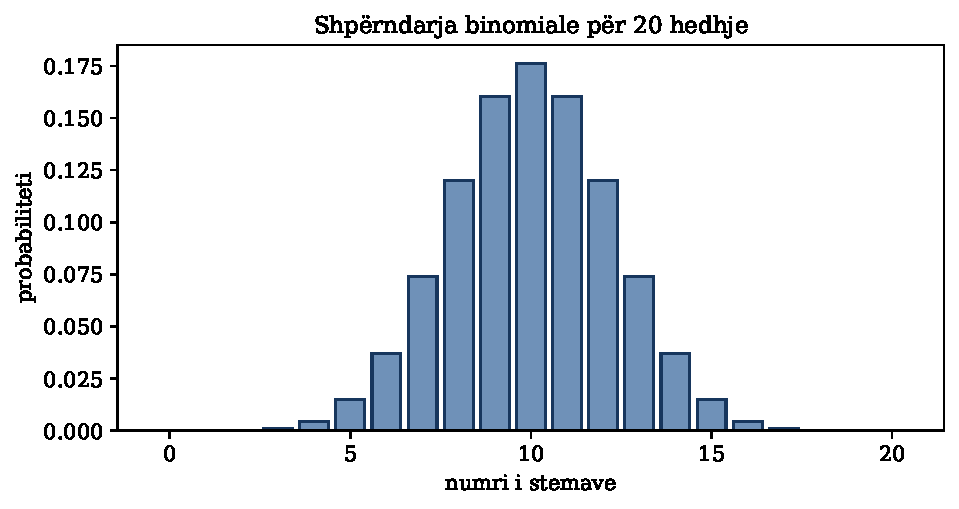
\includegraphics[width=.74\textwidth]{14_shperndarja_binomiale.pdf}
\caption{Shpërndarja e numrit të stemave në 20 hedhje të një monedhe të paanshme.}
\end{figure}

Poisson përshkruan numërime të rralla me normë $\lambda$: $P(K=k)=e^{-\lambda}\lambda^k/k!$. Eksponencialja përshkruan kohën ndërmjet ngjarjeve Poisson dhe ka vetinë pa kujtesë. Gauss-i del nga mbledhja e shumë kontributeve të vogla; parametrat e tij janë mesatarja dhe varianca.

\section{Kovarianca dhe përhapja e pacaktueshmërisë}
\begin{equation}
 \Cov(X,Y)=\E[(X-\E X)(Y-\E Y)],\qquad
 \rho=\frac{\Cov(X,Y)}{\sigma_X\sigma_Y}.
\end{equation}
Për $z=f(\vect x)$ dhe pacaktueshmëri të vogla,
\begin{equation}
 \Var(z)\approx \nabla f^T\Sigma\nabla f,
\end{equation}
ku $\Sigma$ është matrica e kovariancës. Termat jashtë diagonales nuk mund të hiqen kur hyrjet janë të korreluara.

\section{Ligji i numrave të mëdhenj dhe CLT}
Mesatarja e mostrës
\begin{equation}
 \bar X_N=\frac1N\sum_{i=1}^NX_i
\end{equation}
afrohet te $\mu$. Për variancë të fundme, teorema qendrore kufitare jep
\begin{equation}
 \frac{\sqrt N(\bar X_N-\mu)}{\sigma}\Rightarrow\mathcal N(0,1).
\end{equation}
Gabimi standard është $s/\sqrt N$. Katërfishimi i mostrave përgjysmon gabimin, një ligj që përcakton koston e Monte Carlo-s.

\begin{figure}[ht]
\centering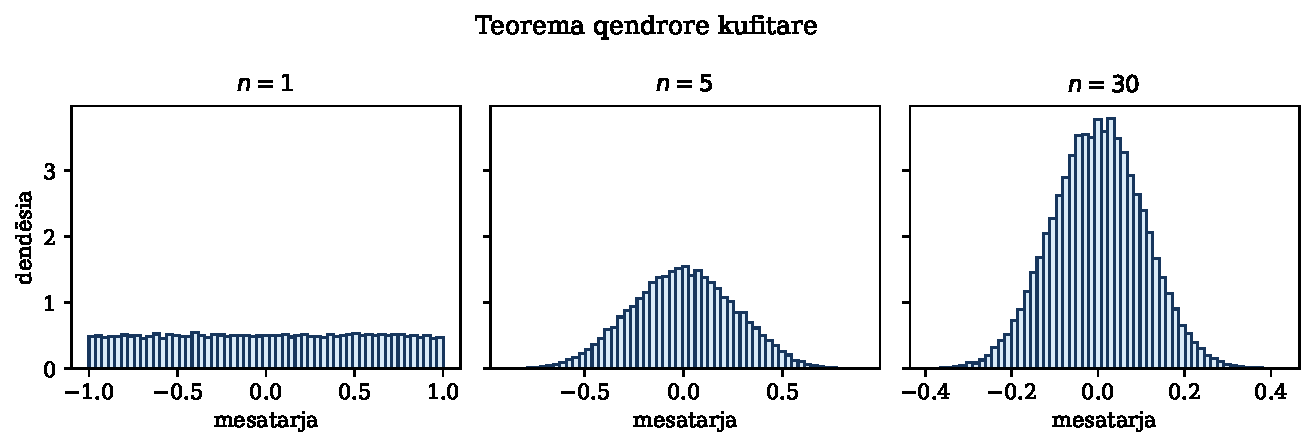
\includegraphics[width=.95\textwidth]{15_teorema_qendrore.pdf}
\caption{Shpërndarja e mesatares së ndryshoreve uniforme afrohet me formën Gauss kur rritet numri i termave.}
\end{figure}

\begin{kujdes}
Formula $s/\sqrt N$ kërkon mostra të pavarura ose një korrigjim për korrelacionin. Në seri Markov, madhësia efektive e mostrës mund të jetë shumë më e vogël se $N$.
\end{kujdes}

\begin{lidhje}
Laboratori simulon hedhjen e monedhës, ndërton intervale besimi dhe kontrollon shkallëzimin $N^{-1/2}$. Diskutohet dallimi ndërmjet luhatjes fizike dhe gabimit të vlerësuesit.
\end{lidhje}

\section*{Pyetje kontrolli}
\begin{enumerate}
\item Dalloni devijimin standard të popullatës nga gabimi standard i mesatares.
\item Kur kovarianca është thelbësore në përhapjen e pacaktueshmërisë?
\item Pse CLT nuk garanton konvergjencë të shpejtë për çdo shpërndarje?
\end{enumerate}
\section{Algoritmet bazë të simulimit probabilitar}
\subsection{Hedhja e monedhës}
\begin{lstlisting}[language=Python,caption={Vlerësimi i probabilitetit dhe gabimit standard.}]
import numpy as np

def monedha(N, p=0.5, seed=2026):
    rng = np.random.default_rng(seed)
    x = rng.random(N) < p
    p_hat = x.mean()
    se = np.sqrt(p_hat*(1-p_hat)/N)
    return p_hat, se, x

for N in [100, 1_000, 10_000, 100_000]:
    p_hat, se, _ = monedha(N)
    print(N, p_hat, se)
\end{lstlisting}
Vlerësimi duhet përsëritur për shumë fara për të parë shpërndarjen e $\hat p$, jo vetëm një trajektore të vetme.

\subsection{Intervali Wilson}
Intervali normal $\hat p\pm z\sqrt{\hat p(1-\hat p)/N}$ sillet dobët për $N$ të vogël ose $\hat p$ pranë 0 e 1. Intervali Wilson është më i qëndrueshëm:
\begin{equation}
 \frac{\hat p+z^2/(2N)\pm z\sqrt{\hat p(1-\hat p)/N+z^2/(4N^2)}}{1+z^2/N}.
\end{equation}

\begin{lstlisting}[language=Python]
def interval_wilson(k, n, z=1.96):
    phat = k/n
    den = 1 + z*z/n
    q = phat + z*z/(2*n)
    d = z*np.sqrt(phat*(1-phat)/n + z*z/(4*n*n))
    return (q-d)/den, (q+d)/den
\end{lstlisting}

\subsection{Përhapja Monte Carlo e pacaktueshmërisë}
\begin{lstlisting}[language=Python,caption={Përhapja e hyrjeve të korreluara.}]
rng = np.random.default_rng(7)
mu = np.array([10.0, 2.0])
Sigma = np.array([[0.25, 0.08], [0.08, 0.04]])
x = rng.multivariate_normal(mu, Sigma, size=200_000)
z = x[:, 0] / x[:, 1]**2
print(np.mean(z), np.std(z), np.quantile(z, [0.025, 0.975]))
\end{lstlisting}
Krahasimi me linearizimin $\nabla f^T\Sigma\nabla f$ tregon kur jolineariteti dhe asimetria bëhen të rëndësishme.

\subsection{Kontrolli i CLT-së}
Për çdo $N$ gjenerohen shumë eksperimente të pavarura dhe studiohet
\begin{equation}
 Z=\frac{\sqrt N(\bar X-\mu)}{\sigma}.
\end{equation}
Histogrami i $Z$ krahasohet me Gauss-in standard. Termi i rekomanduar është \emph{shpërndarje normale} ose \emph{Gauss}, jo përkthime jo të qëndrueshme.

\begin{kujdes}
\emph{Luhatje} përshkruan variacionin e një madhësie të rastit; \emph{gabim standard} përshkruan pacaktueshmërinë e një vlerësuesi. Ato nuk janë sinonime.
\end{kujdes}

Për probabilitetin, statistikën dhe terminologjinë e vlerësimit janë konsultuar materiale universitare shqip \cite{capollari,butka,tasho}; lidhja me simulimin fizik mbështetet te \cite{newman,landau}.

\subsection{Nga aksiomat te ndryshorja e rastit}
Një hapësirë probabilitare $(\Omega,\mathcal F,P)$ përbëhet nga rezultatet e mundshme, ngjarjet e matshme dhe masa e probabilitetit. Ndryshorja e rastit $X:\Omega\to\R$ e shndërron rezultatin elementar në madhësi numerike. Për një ndryshore diskrete,
\begin{equation}
 \E[g(X)]=\sum_x g(x)p_X(x),
\end{equation}
ndërsa për një ndryshore të vazhdueshme,
\begin{equation}
 \E[g(X)]=\int_{-\infty}^{\infty}g(x)f_X(x)\dd x.
\end{equation}
Varianca del nga identiteti
\begin{equation}
 \Var(X)=\E[(X-\mu)^2]=\E[X^2]-\mu^2.
\end{equation}
Ajo ka njësinë në katror të $X$; devijimi standard ka të njëjtën njësi si madhësia fizike.

\subsection{Hedhja e monedhës dhe shpërndarja binomiale}
Le të jetë $X_i\in\{0,1\}$ treguesi i suksesit me $P(X_i=1)=p$. Për prova të pavarura, $S_N=\sum_iX_i$ ka shpërndarje binomiale. Numri i vargjeve me $k$ suksese është $\binom Nk$, prandaj
\begin{equation}
 P(S_N=k)=\binom Nk p^k(1-p)^{N-k}.
\end{equation}
Nga lineariteti i pritjes dhe pavarësia,
\begin{equation}
 \E[S_N]=Np,\qquad \Var(S_N)=Np(1-p).
\end{equation}
Vlerësuesi $\widehat p=S_N/N$ është i paanshëm dhe ka variancë $p(1-p)/N$. Kështu gabimi standard ulet si $N^{-1/2}$, jo si $N^{-1}$.

\subsection{Ligji i numrave të mëdhenj dhe teorema qendrore kufitare}
Ligji i numrave të mëdhenj pohon se mesatarja e mostrës $\overline X_N$ afrohet me $\mu$ kur $N$ rritet. Teorema qendrore kufitare jep më shumë: për ndryshore të pavarura me variancë të fundme,
\begin{equation}
 \frac{\sqrt N(\overline X_N-\mu)}{\sigma}
 \xrightarrow{d}\mathcal N(0,1).
\end{equation}
Kjo justifikon intervalin asimptotik $\overline X\pm z_{1-\alpha/2}s/\sqrt N$. Për mostra të vogla me variancë të panjohur përdoret shpërndarja Student. Për Bernoulli me $p$ pranë zeros ose njësisë, intervali normal mund të dalë jashtë $[0,1]$; intervali Wilson ka sjellje më të mirë.

\subsection{Kovarianca dhe përhapja e pacaktueshmërisë}
Për vektorin $\vect X$ me kovariancë $\Sigma$ dhe $Y=g(\vect X)$, linearizimi rreth mesatares jep
\begin{equation}
 g(\vect X)\simeq g(\vect\mu)+\nabla g(\vect\mu)^T(\vect X-\vect\mu),
\end{equation}
prandaj
\begin{equation}
 \Var(Y)\simeq\nabla g(\vect\mu)^T\Sigma\nabla g(\vect\mu).
\end{equation}
Termat jashtë diagonales mund ta rrisin ose ta ulin pacaktueshmërinë. Supozimi i pavarësisë pa argument mund të jetë po aq problematik sa neglizhimi i një burimi gabimi.

Kur linearizimi nuk është i mjaftueshëm, përhapja Monte Carlo gjeneron $\vect X^{(r)}$ nga shpërndarja e hyrjeve dhe llogarit $Y^{(r)}=g(\vect X^{(r)})$. Shpërndarja empirike e $Y$ mund të jetë asimetrike; atëherë raportohen kuantilet dhe jo vetëm mesatarja me devijimin standard.

\begin{lstlisting}[language=Python,caption={Përhapje Monte Carlo e hyrjeve të korreluara.}]
import numpy as np

rng = np.random.default_rng(2026)
mes = np.array([2.0, 3.0])
kov = np.array([[0.04, 0.03],
                [0.03, 0.09]])
x = rng.multivariate_normal(mes, kov, size=100_000)
y = x[:, 0]**2 / x[:, 1]
q025, q50, q975 = np.quantile(y, [0.025, 0.5, 0.975])
print(q50, q025, q975)
\end{lstlisting}

\subsection{Përmbledhje dhe ushtrime}
Probabiliteti përshkruan modelin e rastësisë; statistika përdor të dhënat për të nxjerrë përfundime rreth këtij modeli. Pacaktueshmëria e rezultatit duhet lidhur me një procedurë kampionimi dhe me supozimet e saj.
\begin{enumerate}
\item Nxirrni mesataren dhe variancën e binomiales nga funksioni gjenerues i momenteve.
\item Krahasoni intervalin normal dhe Wilson për $k=1$ sukses në $N=20$ prova.
\item Provoni me simulim shkallëzimin $N^{-1/2}$ dhe shpjegoni shpërndarjen e pjerrësive të matura.
\item Për periodën $T=2\pi\sqrt{L/g}$, nxirrni përhapjen lineare të pacaktueshmërisë dhe krahasojeni me Monte Carlo.
\end{enumerate}

\subsection{Vlerësuesi, animi dhe gabimi kuadratik mesatar}
Një vlerësues $\widehat\theta$ është ndryshore rasti sepse varet nga mostra. Animi është
\begin{equation}
 \operatorname{Bias}(\widehat\theta)=\E[\widehat\theta]-\theta.
\end{equation}
Gabimi kuadratik mesatar ndahet si
\begin{equation}
 \E[(\widehat\theta-\theta)^2]
 =\Var(\widehat\theta)+\operatorname{Bias}(\widehat\theta)^2.
\end{equation}
Ky identitet tregon se vlerësuesi i paanshëm nuk është automatikisht optimal: një anim i vogël mund të pranohet nëse ul ndjeshëm variancën. Në simulimet fizike, kjo shfaqet te rregullimi i modeleve, prerja e peshave ekstreme ose vlerësuesit me kontroll variabël.

Varianca e mostrës me emërues $N-1$ është e paanshme për variancën e popullatës kur mostrat janë të pavarura,
\begin{equation}
 s^2=\frac{1}{N-1}\sum_{i=1}^{N}(X_i-\overline X)^2.
\end{equation}
Emëruesi $N-1$ vjen sepse mbetjet kanë shumën zero dhe vetëm $N-1$ shkallë lirie. Për seri të korreluara, formula ende përshkruan shpërndarjen margjinale, por $s/\sqrt N$ nuk është gabimi standard i mesatares.

\subsubsection{Intervalet e besimit dhe interpretimi}
Një interval besimi $95\%$ nuk do të thotë se, pasi të dhënat janë vëzhguar, parametri fiks ka probabilitet $95\%$ të jetë brenda atij intervali. Interpretimi frekuentist është se procedura prodhon intervale që mbulojnë parametrin në $95\%$ të përsëritjeve ideale. Ky dallim është i rëndësishëm në raportim.

Për një mesatare me variancë të panjohur dhe të dhëna Gauss të pavarura,
\begin{equation}
 \frac{\overline X-\mu}{s/\sqrt N}\sim t_{N-1}.
\end{equation}
Për mostra të mëdha, kuantilet $t$ afrohen me ato normale. Për probabilitete binomiale, intervali Wilson ose një interval i bazuar në gjasë është më i qëndrueshëm se intervali Wald, sidomos pranë kufijve.

\subsubsection{Bootstrap-i}
Bootstrap-i joparametrik trajton shpërndarjen empirike si përafrim të popullatës. Nga mostra origjinale me $N$ elemente krijohen mostra të reja me rizgjedhje dhe të njëjtën madhësi. Për secilën llogaritet statistiku $T^{*(b)}$. Shpërndarja e këtyre statistikëve vlerëson variancën, animin dhe intervalet.

Metoda funksionon mirë për shumë statistikë të lëmuar, por nuk është universale. Për maksimumin, bishtat ekstremë dhe mostra shumë të vogla mund të jetë e dobët. Për seri kohore nuk duhet rizgjedhur çdo pikë veçmas, sepse prishet varësia; përdoret bootstrap në blloqe. Në Monte Carlo me peshë, skema e rizgjedhjes duhet të respektojë mënyrën si u krijuan peshat.

\subsubsection{Kovarianca nga burime të përbashkëta}
Në eksperimente fizike, dy madhësi shpesh varen nga i njëjti kalibrim. Nëse $x=x_0(1+\epsilon)$ dhe $y=y_0(1+\epsilon)$ ndajnë të njëjtin gabim relativ, raporti $x/y$ anulon gabimin e përbashkët në rendin e parë. Trajtimi i $x$ dhe $y$ si të pavarura do ta mbivlerësonte pacaktueshmërinë. Në diferencën $x-y$, i njëjti korrelacion mund ta ulë ose ta rrisë efektin në varësi të shenjave.

Matrica e kovariancës duhet të jetë simetrike pozitivisht gjysmë e përcaktuar. Një matricë e ndërtuar nga koeficientë korrelacioni të papajtueshëm mund të ketë vlera vetjake negative dhe të mos përfaqësojë asnjë shpërndarje. Para kampionimit shumënormal kontrollohen simetria dhe spektri; vlera të vogla negative nga rrumbullakimi mund të kërkojnë korrigjim të dokumentuar.

\subsubsection{Ligji total i variancës}
Kur modeli varet nga parametri i rastit $\Theta$ dhe nga zhurma e brendshme,
\begin{equation}
 \Var(Y)=\E[\Var(Y\mid\Theta)]
 +\Var(\E[Y\mid\Theta]).
\end{equation}
Termi i parë mat variabilitetin brenda realizimeve për parametra të fiksuar; i dyti mat ndryshimin ndërmjet parametrave. Kjo ndarje është e dobishme në simulimin e zbritjes së mjetit hapësinor, ku mund të dallohen ndryshimet atmosferike nga zhurma e sensorit ose e kontrollit.


\chapter{Numrat pseudorastësorë dhe kampionimi}
\begin{qellime}
Studenti shpjegon gjeneratorët pseudorastësorë, farën dhe gjendjen; zbaton transformimin e anasjelltë, Box--Muller dhe kampionimin me refuzim; teston shpërndarjen dhe pavarësinë; shmang përdorimin e gabuar paralel.
\end{qellime}

\section{Pseudo-rastësia}
Një gjenerator pseudorastësor është algoritëm determinist që prodhon një varg me veti statistike të ngjashme me mostrat e pavarura uniforme. Gjeneratori kongruencial linear është
\begin{equation}
 x_{n+1}=(ax_n+c)\bmod m,\qquad u_n=x_n/m.
\end{equation}
Zgjedhja e parametrave përcakton periodën dhe korrelacionet. Gjeneratorët modernë kanë gjendje më të madhe dhe teste më të mira, por nuk janë automatikisht kriptografikisht të sigurt.

Fara përcakton vargun. Ruajtja e saj mundëson riprodhim. Megjithatë, përdorimi i të njëjtës farë në procese paralele mund të krijojë vargje identike; duhen nënrryma të pavarura ose mekanizma \emph{spawn}.

\begin{figure}[ht]
\centering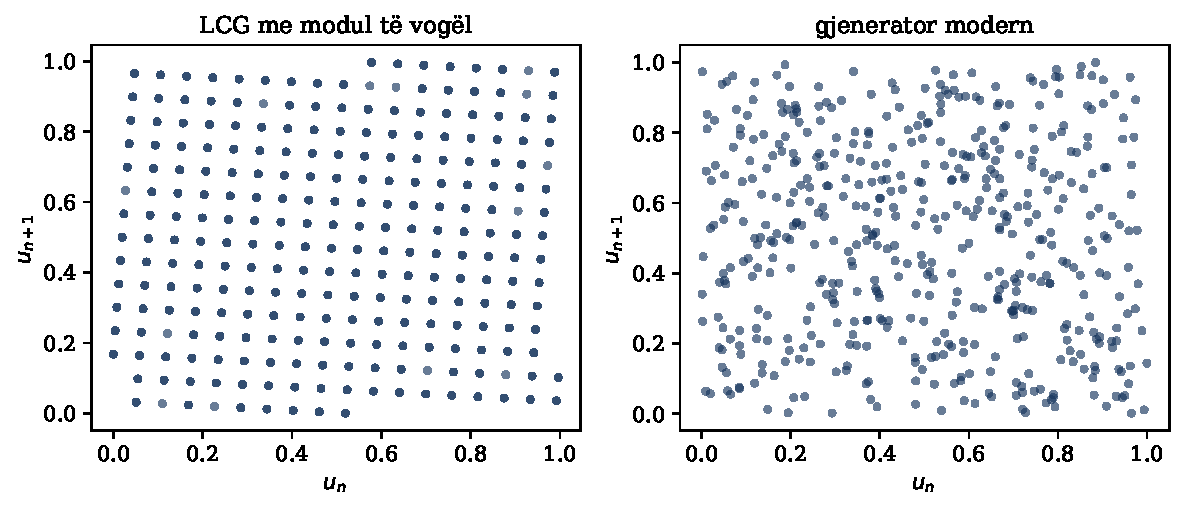
\includegraphics[width=.90\textwidth]{16_testi_cifteve_prng.pdf}
\caption{Grafiku $(u_n,u_{n+1})$ zbulon strukturë rrjete në një gjenerator të dobët.}
\end{figure}

\section{Testet statistike}
Histogrami kontrollon uniformitetin njëpërmasor, por nuk zbulon çdo varësi. Përdoren testi $\chi^2$, Kolmogorov--Smirnov, autokorrelacioni dhe teste spektrale. Një vlerë-$p$ nuk provon rastësinë; ajo vetëm mat përputhjen me një statistikë të zgjedhur. Testimi duhet të përfshijë shumë struktura dhe gjatësi vargu.

\section{Transformimi i anasjelltë}
Nëse $U\sim\mathcal U(0,1)$ dhe $F$ është kumulativi i synuar, atëherë
\begin{equation}
 X=F^{-1}(U)
\end{equation}
ka shpërndarje $F$. Për eksponencialen me normë $\lambda$,
\begin{equation}
 X=-\frac1\lambda\ln(1-U).
\end{equation}

\begin{figure}[ht]
\centering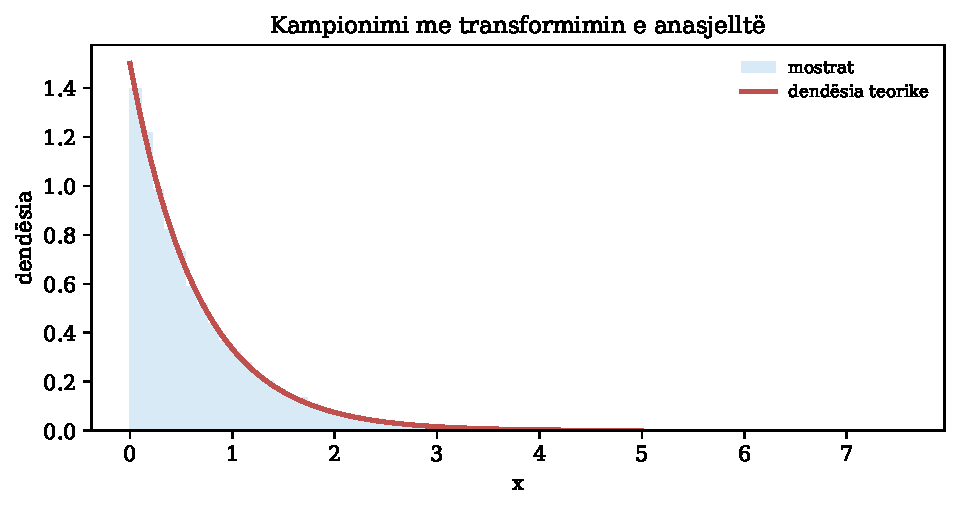
\includegraphics[width=.74\textwidth]{17_kampionimi_eksponencial.pdf}
\caption{Mostrat e gjeneruara me transformimin e anasjelltë dhe dendësia teorike.}
\end{figure}

\section{Mostrat Gauss}
Transformimi Box--Muller përdor dy uniforme të pavarura:
\begin{align}
 Z_1&=\sqrt{-2\ln U_1}\cos(2\pi U_2),\\
 Z_2&=\sqrt{-2\ln U_1}\sin(2\pi U_2).
\end{align}
Kjo rrjedh nga kalimi në koordinata polare të dendësisë Gauss dydimensionale. Bibliotekat moderne mund të përdorin algoritme më të shpejta, por parimi mbetet shembull i rëndësishëm i transformimit të ndryshoreve.

\section{Kampionimi me refuzim}
Le të jetë $f(x)$ dendësia synuar dhe $g(x)$ propozimi, me $f(x)\le Mg(x)$. Gjenerohet $X\sim g$ dhe pranohet nëse
\begin{equation}
 U\le\frac{f(X)}{Mg(X)}.
\end{equation}
Norma mesatare e pranimit është $1/M$. Propozimi duhet të mbulojë të gjithë mbështetjen e $f$ dhe bishtat e tij nuk duhet të jenë më të lehtë. Në dimension të lartë, refuzimi global bëhet shpesh joefikas.

\section{Kampionimi i rëndësisë}
Për një pritje nën $p$,
\begin{equation}
 \E_p[h(X)]=\int h(x)\frac{p(x)}{q(x)}q(x)\dd x
 \approx\frac1N\sum_{i=1}^Nh(X_i)w(X_i),\quad X_i\sim q.
\end{equation}
Propozimi $q$ duhet të vendosë mostra atje ku $|h|p$ është i madh. Peshat shumë të pabarabarta japin madhësi të vogël efektive të mostrës,
\begin{equation}
 N_{\mathrm{eff}}\approx\frac{(\sum_iw_i)^2}{\sum_iw_i^2}.
\end{equation}

\begin{kujdes}
Ndryshimi i farës nuk zëvendëson analizën statistike. Rezultati duhet të jetë i qëndrueshëm ndaj disa farave, ndërsa raportimi duhet të japë vlerësuesin dhe gabimin standard.
\end{kujdes}

\begin{lidhje}
Laboratori gjeneron uniforme, eksponenciale dhe Gauss; përdor histogramin, CDF empirike dhe autokorrelacionin; krahason transformimin e anasjelltë me refuzimin.
\end{lidhje}

\section*{Pyetje kontrolli}
\begin{enumerate}
\item Pse një histogram uniform nuk provon pavarësinë?
\item Çfarë ndodh nëse $Mg(x)<f(x)$ në një zonë?
\item Si organizohen vargjet pseudorastësore në llogaritje paralele?
\end{enumerate}
\section{Algoritmet e gjenerimit dhe kampionimit}
\subsection{Gjeneratori dhe gjendja e tij}
Në NumPy rekomandohet objekti \texttt{Generator}. Ai e bën burimin e rastësisë të dukshëm dhe shmang varësinë nga një gjendje globale.
\begin{lstlisting}[language=Python]
rng = np.random.default_rng(2026)
u = rng.random(1_000_000)
print(u.mean(), u.var())  # priten afersisht 1/2 dhe 1/12
\end{lstlisting}

\subsection{Transformimi i anasjelltë}
\begin{lstlisting}[language=Python,caption={Mostra eksponenciale pa përdorur funksionin e gatshëm.}]
def eksponenciale_anasjelltas(rng, lam, size):
    u = rng.random(size)
    return -np.log1p(-u) / lam

x = eksponenciale_anasjelltas(rng, lam=1.5, size=100_000)
print(x.mean(), 1/1.5)
\end{lstlisting}
Funksioni \texttt{log1p(-u)} është më i saktë kur $u$ është i vogël. Kontrollohen mesatarja, varianca dhe CDF-ja empirike.

\subsection{Box--Muller}
\begin{lstlisting}[language=Python,caption={Gjenerimi i çifteve Gauss standarde.}]
def box_muller(rng, n):
    u1 = rng.random(n)
    u2 = rng.random(n)
    r = np.sqrt(-2.0*np.log(u1))
    phi = 2.0*np.pi*u2
    return r*np.cos(phi), r*np.sin(phi)
\end{lstlisting}
Testohet jo vetëm histogrami i secilit komponent, por edhe kovarianca ndërmjet tyre.

\subsection{Kampionimi me refuzim}
\begin{lstlisting}[language=Python,caption={Refuzimi për një dendësi në interval të fundmë.}]
def refuzim(rng, f, a, b, M, n):
    pranuar = []
    prova = 0
    while len(pranuar) < n:
        x = rng.uniform(a, b)
        y = rng.uniform(0.0, M)
        prova += 1
        if y <= f(x):
            pranuar.append(x)
    return np.asarray(pranuar), n/prova
\end{lstlisting}
Këtu $M$ është kufi i sipërm i $f$ në $[a,b]$. Në formulimin me propozim të përgjithshëm, kontrollohet $f(x)\le M g(x)$.

\subsection{Testet minimale}
\begin{enumerate}
\item krahasohen momentet empirike me ato teorike;
\item vizatohet CDF-ja empirike;
\item testohet autokorrelacioni;
\item përsëritet me fara të ndryshme;
\item matet norma e pranimit dhe kostoja për mostër.
\end{enumerate}
Termi \emph{kampionim} përdoret për sampling dhe \emph{mostër} për sample. \emph{Gjenerator pseudorastësor} thekson natyrën deterministe të vargut.

Terminologjia probabilitare shqip mbështetet te \cite{capollari,butka,tasho}; algoritmet e gjenerimit dhe testimit krahasohen me trajtimet standarde \cite{press,robert}.

\subsection{Gjeneratorët pseudorastësorë si sisteme dinamike diskrete}
Një gjenerator pseudorastësor është një algoritëm determinist me gjendje të fundme. Gjeneratori kongruencial linear,
\begin{equation}
 x_{n+1}=(ax_n+c)\bmod m,
 \qquad u_n=\frac{x_n}{m},
\end{equation}
e bën këtë strukturë të dukshme. Për shkak se ka vetëm $m$ gjendje, vargu duhet të përsëritet; perioda dhe korrelacionet varen nga parametrat. Edhe kur histogrami i $u_n$ duket uniform, çiftet $(u_n,u_{n+1})$ mund të shtrihen në një numër të vogël hiperplanesh. Prandaj uniformiteti njëpërmasor nuk provon cilësinë shumëpërmasore.

Gjeneratorët modernë kanë gjendje shumë më të madhe dhe cilësi të testuar, por mbeten deterministë. Fara përcakton trajektoren. Ruajtja e farës siguron riprodhueshmëri, ndërsa përdorimi i së njëjtës farë për eksperimente që duhet të jenë të pavarura mund të krijojë korrelacione artificiale.

\subsection{Transformimi i anasjellë}
Nëse $U\sim\mathcal U(0,1)$ dhe $F$ është funksioni kumulativ i vazhdueshëm e rritës, atëherë
\begin{equation}
 X=F^{-1}(U)
\end{equation}
ka funksion kumulativ $F$, sepse
\begin{equation}
 P(X\le x)=P(F^{-1}(U)\le x)=P(U\le F(x))=F(x).
\end{equation}
Për eksponencialen $F(x)=1-e^{-\lambda x}$ merret
\begin{equation}
 X=-\frac{1}{\lambda}\ln(1-U).
\end{equation}
Shkrimi $\log1p(-U)$ është më i saktë kur $U$ është i vogël. Metoda është e thjeshtë kur inversi është i njohur; për shpërndarje të tjera nevojitet zgjidhje numerike ose metodë alternative.

\subsection{Box--Muller për mostrën Gauss}
Dy ndryshore Gauss standarde kanë dendësi të përbashkët
\begin{equation}
 f(z_1,z_2)=\frac{1}{2\pi}\exp[-(z_1^2+z_2^2)/2].
\end{equation}
Në koordinata polare, elementi i sipërfaqes është $r\dd r\dd\theta$, kështu që $\Theta$ është uniforme në $[0,2\pi)$ dhe $R^2$ ka shpërndarje eksponenciale me parametër $1/2$. Me $U_1,U_2$ uniforme të pavarura,
\begin{equation}
 R=\sqrt{-2\ln U_1},\qquad \Theta=2\pi U_2,
\end{equation}
dhe
\begin{equation}
 Z_1=R\cos\Theta,qquad Z_2=R\sin\Theta.
\end{equation}
Duhet shmangur $U_1=0$. Mostrat verifikohen jo vetëm me histogram, por edhe me mesatare, variancë, kuantile dhe korrelacion ndërmjet $Z_1$ e $Z_2$.

\subsection{Kampionimi me refuzim}
Le të jetë $f$ dendësia e synuar dhe $g$ dendësia propozuese, me $f(x)\le Mg(x)$. Gjenerohet $Y\sim g$ dhe $U\sim\mathcal U(0,1)$; $Y$ pranohet kur
\begin{equation}
 U\le\frac{f(Y)}{Mg(Y)}.
\end{equation}
Dendësia e një vlere të pranuar është proporcionale me
\begin{equation}
 g(y)\frac{f(y)}{Mg(y)}=\frac{f(y)}{M},
\end{equation}
pra pas normalizimit është $f$. Probabiliteti mesatar i pranimit është $1/M$. Një mbështjellëse e dobët e bën metodën të kushtueshme, sidomos në dimension të lartë.

\subsection{Kampionimi i rëndësisë dhe madhësia efektive}
Për një pritje nën $p$,
\begin{equation}
 I=\int h(x)p(x)\dd x
 =\int h(x)\frac{p(x)}{q(x)}q(x)\dd x,
\end{equation}
gjenerohen $X_i\sim q$ dhe përdoren peshat $w_i=p(X_i)/q(X_i)$. Kushti themelor është që $q>0$ kudo ku $|h|p$ kontribuon. Varianca mund të zvogëlohet shumë nëse $q$ vendos mostra në rajonet me kontribut të madh, por peshat shumë të pabarabarta e bëjnë vlerësimin të paqëndrueshëm. Një diagnostikë është
\begin{equation}
 N_{\mathrm{eff}}=\frac{(\sum_iw_i)^2}{\sum_iw_i^2}.
\end{equation}
Kjo nuk është identike me madhësinë efektive të një zinxhiri Markov, megjithëse të dyja matin humbjen e informacionit kundrejt $N$ mostrave ideale.

\subsection{Testimi i mostrave}
Një paketë minimale kontrollesh përfshin histogramin, CDF-në empirike, testin e momenteve dhe autokorrelacionin. Vlera-$p$ nuk provon rastësinë; ajo mat sa i pazakontë është statistiku nën një hipotezë të caktuar. Me shumë teste shfaqen rezultate të vogla edhe për një gjenerator të mirë, prandaj duhet parë modeli i përgjithshëm dhe jo vetëm minimumi i vlerave-$p$.

\subsection{Përmbledhje dhe ushtrime}
Gjenerimi i mostrës është pjesë e algoritmit shkencor. Një transformim i saktë matematikisht mund të dështojë numerikisht ose të trashëgojë korrelacionet e gjeneratorit bazë.
\begin{enumerate}
\item Gjeni kushtet për periodë të plotë të një gjeneratori kongruencial linear dhe testojini në parametra të vegjël.
\item Nxirrni transformimin e anasjellë për shpërndarjen Pareto.
\item Vërtetoni Box--Muller-in duke përfshirë Jakobinin polar.
\item Ndërtoni një mbështjellëse refuzimi për një dendësi trekëndore dhe parashikoni normën e pranimit.
\item Krahasoni dy propozime të kampionimit të rëndësisë me anë të variancës dhe $N_{\mathrm{eff}}$.
\end{enumerate}

\subsection{Rrymat e pavarura dhe ekzekutimi paralel}
Në një simulim paralel, përdorimi i farave $s,s+1,s+2,\ldots$ nuk garanton rryma të pavarura për çdo familje gjeneratorësh. Gjeneratorët modernë ofrojnë mekanizma për ndarje: kapërcim përpara, nënrryma ose ndërtim të gjendjeve fëmijë nga një sekuencë farash. Qëllimi është që asnjë punëtor të mos përdorë pjesë të mbivendosura të të njëjtit varg.

Rezultati duhet të jetë i riprodhueshëm edhe kur ndryshon numri i bërthamave. Një strategji është që çdo realizim të marrë farë të derivuar nga identifikuesi i realizimit, jo nga rendi i ekzekutimit. Atëherë planifikimi paralel mund të ndryshojë pa ndryshuar mostrat. Në raport ruhen fara bazë, metoda e ndarjes dhe versioni i bibliotekës.

Gjeneratori kriptografik nuk është domosdoshmërisht i nevojshëm për fizikë llogaritëse; kërkohen periodë e gjatë, cilësi statistikë, shpejtësi dhe ndarje e sigurt e rrymave. Për aplikime sigurie, parashikueshmëria deterministe është e papranueshme dhe kërkesat janë të tjera.

\subsubsection{Gjenerimi i vektorëve Gauss të korreluar}
Le të jetë $\vect Z\sim\mathcal N(0,I)$ dhe $\Sigma=LL^T$ faktorizimi Cholesky i kovariancës. Atëherë
\begin{equation}
 \vect X=\vect\mu+L\vect Z
\end{equation}
ka mesatare $\vect\mu$ dhe kovariancë
\begin{equation}
 \Cov(\vect X)=L\Cov(\vect Z)L^T=LL^T=\Sigma.
\end{equation}
Nëse $\Sigma$ është vetëm pozitivisht gjysmë e përcaktuar, Cholesky mund të dështojë; përdoret zbërthimi spektral dhe mbahen vlerat vetjake jo negative. Një vlerë vetjake zero përfaqëson kufizim të saktë linear dhe dimension efektiv më të vogël.

Kontrolli empirik kërkon shumë realizime dhe krahasim të mesatares e kovariancës së mostrës me objektivat. Devijimet priten të shkallëzohen me madhësinë e mostrës; nuk duhet kërkuar barazi e saktë. Grafikët e çifteve ndihmojnë të zbulohen shenja të gabuara ose renditje e gabuar e komponentëve.

\subsubsection{Metoda e përbërjes dhe shpërndarjet diskrete}
Nëse dendësia është përzierje
\begin{equation}
 f(x)=\sum_{k=1}^{K}w_kf_k(x),\qquad w_k\ge0,\quad\sum_kw_k=1,
\end{equation}
fillimisht gjenerohet komponenti $K$ me probabilitete $w_k$, pastaj $X\sim f_K$. Kjo metodë është e saktë dhe shpesh më efikase se refuzimi. Për shembull, një model zhurme me bërthamë të ngushtë dhe bisht të gjerë mund të simulohet si përzierje e dy shpërndarjeve Gauss.

Për shpërndarje diskrete me shumë kategori, kërkimi kumulativ kushton $\Oh(\log K)$ me kërkim binar. Metoda alias kryen parapërpunim $\Oh(K)$ dhe pastaj gjeneron çdo kategori në kohë $\Oh(1)$. Zgjedhja varet nga sa herë përdoret e njëjta shpërndarje.

\subsubsection{Efikasiteti i refuzimit në dimension të lartë}
Në njësi $d$-dimensionale, raporti i vëllimit të sferës ndaj kubit kufizues është
\begin{equation}
 \frac{V_d}{2^d}=\frac{\pi^{d/2}}{2^d\Gamma(d/2+1)},
\end{equation}
dhe shkon shpejt në zero. Prandaj gjenerimi uniform në kub dhe refuzimi jashtë sferës bëhet katastrofik në dimension të lartë. Ky shembull konkret tregon se një algoritëm intuitiv në dy përmasa mund të jetë i papërdorshëm në njëzet përmasa.

Transformimet që respektojnë gjeometrinë, kampionimi i rëndësisë ose MCMC shmangin këtë humbje. Megjithatë, MCMC prodhon korrelacion dhe kërkon diagnostikë; nuk ka metodë universale pa kosto.

\subsubsection{Testet si bateri, jo si vulë}
Një test uniformiteti kontrollon vetëm një aspekt. Testet seriale kontrollojnë çifte ose blloqe; testet spektrale kontrollojnë strukturën e rrjetës; testet e runs kontrollojnë vargjet rritëse dhe zbritëse. Kur kryhen shumë teste në nivel $5\%$, rreth $5\%$ pritet të dështojnë rastësisht. Duhet parë shpërndarja e vlerave-$p$, përsëritja në fara të ndryshme dhe rëndësia për algoritmin konkret.

Prova më bindëse për një simulim është kombinimi i një gjeneratori të njohur, testeve standarde dhe verifikimit të observablave ndaj rezultateve teorike. Një gjenerator mund të kalojë një bateri dhe përsëri të bashkëveprojë keq me strukturën periodike të një algoritmi të veçantë.


\chapter{Integrimi Monte Carlo}
\begin{qellime}
Studenti formulon integralin si pritje; ndërton vlerësuesin Monte Carlo dhe gabimin e tij; përdor kampionim të rëndësisë, variabla antitetike dhe variabla kontrolli; trajton integrale shumëdimensionale dhe pacaktueshmëri në modele fizike.
\end{qellime}

\section{Integrali si pritje}
Për domen $D$ me vëllim $V_D$ dhe mostra uniforme $X_i$,
\begin{equation}
 I=\int_Df(\vect x)\dd\vect x=V_D\E[f(X)],
\qquad
 \hat I_N=\frac{V_D}{N}\sum_{i=1}^Nf(X_i).
\end{equation}
Vlerësuesi është i paanshëm dhe
\begin{equation}
 \operatorname{SE}(\hat I_N)=V_D\frac{\sigma_f}{\sqrt N}.
\end{equation}
Avantazhi kryesor është se rendi $N^{-1/2}$ nuk përkeqësohet drejtpërdrejt me dimensionin. Disavantazhi është konvergjenca e ngadaltë në dimension të ulët krahasuar me kuadraturat me rend të lartë.

\section{Shembulli gjeometrik i $\pi$}
Në katrorin njësi, probabiliteti që $x^2+y^2\le1$ është $\pi/4$. Prandaj
\begin{equation}
 \hat\pi_N=4\frac{N_{\mathrm{brenda}}}{N}.
\end{equation}
Ky shembull është intuitiv, por jo metodë efikase për llogaritjen e $\pi$; shërben për të demonstruar treguesit, ligjin binomial dhe intervalin e besimit.

\begin{figure}[ht]
\centering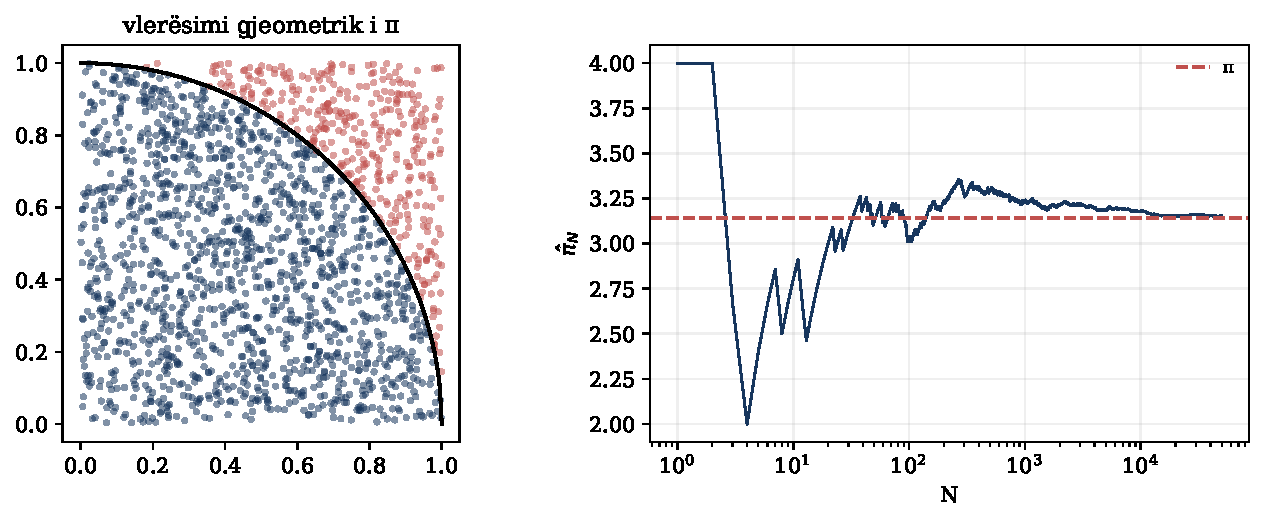
\includegraphics[width=.95\textwidth]{18_monte_carlo_pi.pdf}
\caption{Vlerësimi gjeometrik i $\pi$ dhe konvergjenca e vlerësuesit.}
\end{figure}

\section{Gabimi statistik}
Varianca vlerësohet nga mostrat,
\begin{equation}
 s_f^2=\frac1{N-1}\sum_{i=1}^N(f_i-\bar f)^2,
\qquad \widehat{\operatorname{SE}}(\hat I_N)=V_D\frac{s_f}{\sqrt N}.
\end{equation}
Raportimi $\hat I\pm\mathrm{SE}$ pa treguar $N$, metodën e kampionimit dhe korrelacionin është i paplotë. Për integrandë me variancë të pafundme, CLT standard mund të mos zbatohet.

\begin{figure}[ht]
\centering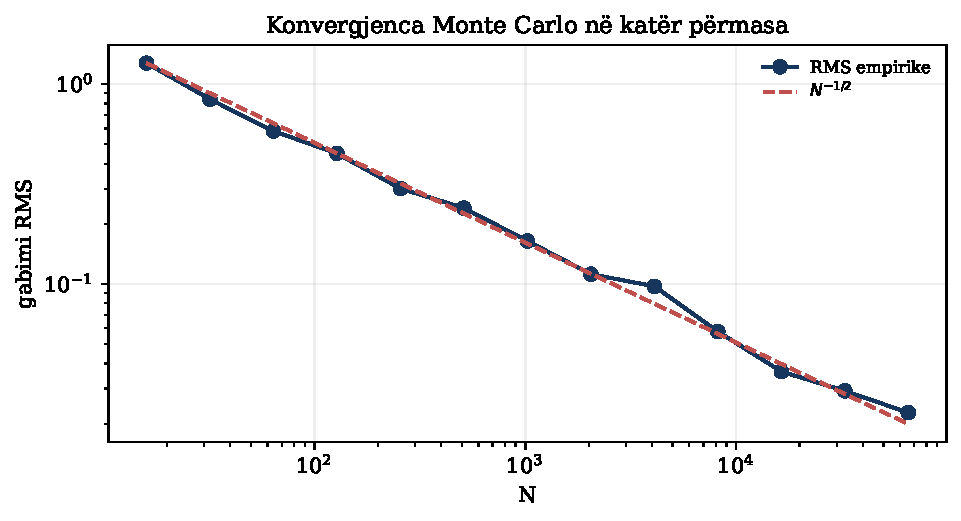
\includegraphics[width=.74\textwidth]{19_gabimi_monte_carlo.pdf}
\caption{Shkallëzimi $N^{-1/2}$ në një integral katërpërmasor.}
\end{figure}

\section{Reduktimi i variancës}
\subsection{Kampionimi i rëndësisë}
Nëse $p$ është dendësia e synuar dhe $q$ dendësia e kampionimit,
\begin{equation}
 I=\E_q\left[f(X)\frac{p(X)}{q(X)}\right].
\end{equation}
Zgjedhja ideale vendos më shumë mostra ku kontributi është i madh. Peshat duhet të monitorohen për degenerim.

\subsection{Variablat antitetike}
Për $U\sim\mathcal U(0,1)$, çiftet $U$ dhe $1-U$ janë të korreluara negativisht për funksione monotone. Mesatarja e çiftit mund të ketë variancë më të vogël se dy mostra të pavarura.

\subsection{Variablat kontrolli}
Nëse $g$ ka pritje të njohur,
\begin{equation}
 \hat I_c=\bar f-c(\bar g-\E g).
\end{equation}
Koeficienti optimal është $c^*=\Cov(f,g)/\Var(g)$. Metoda përdor korrelacionin me një model të thjeshtë për të korrigjuar modelin e shtrenjtë.

\section{Integrale shumëfishta dhe rajone të ndërlikuara}
Një tregues $\mathbf1_D(\vect x)$ e kthen integrimin mbi rajon të parregullt në pritje mbi një kuti. Efikasiteti bie kur $D$ zë fraksion shumë të vogël. Atëherë përdoret parametrizim i rajonit, kampionim i rëndësisë ose ndarje stratifikore.

Quasi-Monte Carlo zëvendëson rastësinë me vargje me diskrepancë të ulët. Për integrandë të rregullt mund të tejkalojë $N^{-1/2}$, por vlerësimi i gabimit kërkon randomizim ose analiza të tjera.

\section{Përhapja Monte Carlo e pacaktueshmërisë}
Kur dalja $Y=g(\vect X)$ varet jolinearisht nga hyrje të pacaktuara, kampionohen hyrjet sipas shpërndarjes së tyre dhe llogaritet $Y$ për çdo realizim. Kjo ruan jo-Gaussianitetin, kufijtë dhe korrelacionet. Shpërndarja e daljes jep kuantile dhe probabilitete rreziku, jo vetëm mesatare.

\begin{figure}[ht]
\centering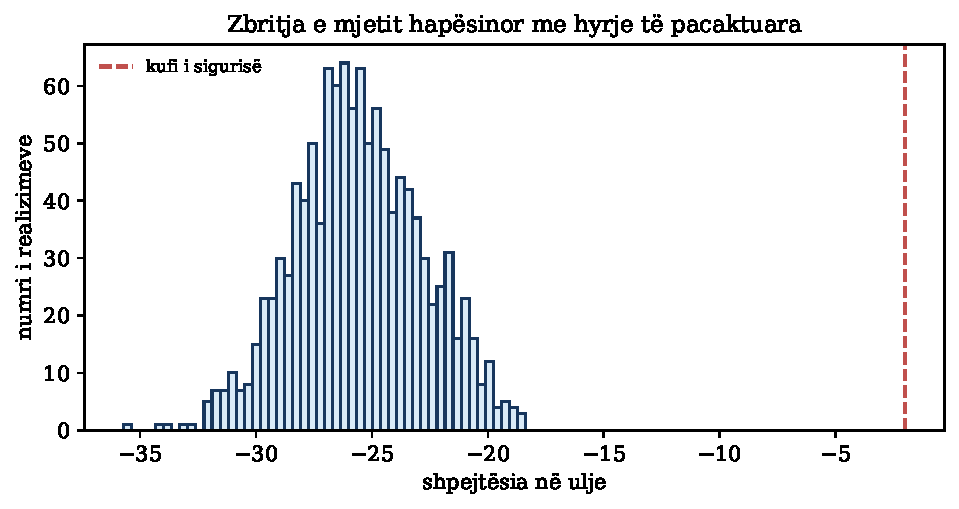
\includegraphics[width=.74\textwidth]{20_zbritja_mjetit_monte_carlo.pdf}
\caption{Shpërndarja e shpejtësisë së uljes kur lartësia, shpejtësia fillestare dhe shtytja kanë pacaktueshmëri.}
\end{figure}

\begin{shembull}[Zbritja e mjetit hapësinor]
Për çdo realizim kampionohen masa, shtytja, lartësia dhe shpejtësia fillestare. Integruesi dinamik jep shpejtësinë e kontaktit. Probabiliteti $P(v_{\mathrm{kontakt}}<v_{\mathrm{kufi}})$ është madhësi më informative se një trajektore me parametra mesatarë.
\end{shembull}

\begin{lidhje}
Laboratori krahason kuadraturën dhe Monte Carlo-n, verifikon $N^{-1/2}$, përdor një teknikë reduktimi variance dhe zbaton përhapjen e pacaktueshmërisë në zbritjen e mjetit.
\end{lidhje}

\section*{Pyetje kontrolli}
\begin{enumerate}
\item Pse Monte Carlo bëhet më tërheqës në dimension të lartë?
\item Si zgjidhet një variabël kontrolli e mirë?
\item Pse simulimi me parametrat mesatarë nuk jep domosdoshmërisht daljen mesatare?
\end{enumerate}
\section{Algoritmet Monte Carlo në Python}
\subsection{Integruesi bazë me gabim standard}
\begin{lstlisting}[language=Python,caption={Integrimi uniform në një kuti shumëpërmasore.}]
def integral_mc(f, kufijte, N, seed=2026):
    rng = np.random.default_rng(seed)
    kufijte = np.asarray(kufijte, float)
    a, b = kufijte[:, 0], kufijte[:, 1]
    x = rng.uniform(a, b, size=(N, len(a)))
    fx = np.asarray(f(x), float)
    vellimi = np.prod(b - a)
    vleresimi = vellimi * fx.mean()
    se = vellimi * fx.std(ddof=1) / np.sqrt(N)
    return vleresimi, se

f = lambda x: np.exp(x.sum(axis=1))
I, se = integral_mc(f, [(0, 1)]*4, N=200_000)
print(f"I = {I:.6f} +/- {se:.6f}")
\end{lstlisting}

\subsection{Kontrolli i ligjit $N^{-1/2}$}
Për secilin $N$ kryhen $R$ simulime të pavarura. Llogaritet RMSE kundrejt një reference dhe përshtatet pjerrësia në koordinata logaritmike.
\begin{lstlisting}[language=Python]
Ns = 2**np.arange(8, 18)
rmse = []
for N in Ns:
    v = [integral_mc(f, [(0, 1)]*4, N, seed=s)[0]
         for s in range(40)]
    rmse.append(np.sqrt(np.mean((np.array(v) - I_ref)**2)))
pjerrtesia = np.polyfit(np.log(Ns), np.log(rmse), 1)[0]
\end{lstlisting}
Pjerrësia pritet afër $-1/2$. Devijimi mund të vijë nga numër i pamjaftueshëm përsëritjesh ose nga variancë e madhe e integrandit.

\subsection{Variabli kontrollues}
\begin{lstlisting}[language=Python,caption={Reduktimi i variancës me një madhësi të korreluar.}]
def kontrolli(fx, gx, Eg):
    cov = np.cov(fx, gx, ddof=1)
    c = cov[0, 1] / cov[1, 1]
    korrigjuar = fx - c*(gx - Eg)
    return korrigjuar.mean(), korrigjuar.std(ddof=1)/np.sqrt(len(fx)), c
\end{lstlisting}
Raportohet faktori i reduktimit të variancës $\Var(f)/\Var(f_c)$. Nëse korrelacioni është i dobët, metoda mund të mos sjellë përfitim.

\subsection{Pacaktueshmëria e zbritjes së mjetit}
Algoritmi i plotë është i folezuar: jashtë kampionohen parametrat; brenda integrohet dinamika për çdo realizim. Rezultati është shpërndarja e shpejtësisë së kontaktit dhe probabiliteti i tejkalimit të kufirit.
\begin{lstlisting}[language=Python]
rng = np.random.default_rng(12)
parametra = rng.multivariate_normal(mu, Sigma, size=20_000)
v_kontakt = np.array([simulo_zbritjen(p) for p in parametra])
rreziku = np.mean(v_kontakt < v_kufi)
se_rreziku = np.sqrt(rreziku*(1-rreziku)/len(v_kontakt))
\end{lstlisting}

\begin{kujdes}
Në shqip dallohen \emph{vlerësuesi} (estimator), \emph{vlerësimi} (estimate), \emph{varianca} dhe \emph{gabimi standard}. Shprehja ``gabimi Monte Carlo'' duhet të shoqërohet me përkufizimin konkret.
\end{kujdes}

Literatura shqip për Monte Carlo është më e kufizuar; për terminologjinë probabilitare dhe të rizgjedhjes janë përdorur \cite{butka,tasho,hyka}, ndërsa baza algoritmike mbështetet te \cite{newman,robert,press}.

\subsection{Integrimi Monte Carlo si vlerësim i një pritjeje}
Le të jetë $X\sim p$ dhe
\begin{equation}
 I=\int h(x)p(x)\dd x=\E_p[h(X)].
\end{equation}
Vlerësuesi bazë është
\begin{equation}
 \widehat I_N=\frac1N\sum_{i=1}^{N}h(X_i).
\end{equation}
Për mostra të pavarura,
\begin{equation}
 \E[\widehat I_N]=I,
 \qquad
 \Var(\widehat I_N)=\frac{\sigma_h^2}{N}.
\end{equation}
Gabimi standard vlerësohet me $s_h/\sqrt N$. Teorema qendrore kufitare jep
\begin{equation}
 \frac{\widehat I_N-I}{s_h/\sqrt N}\approx\mathcal N(0,1).
\end{equation}
Kështu për ta përgjysmuar gabimin duhen afërsisht katër herë më shumë mostra. Shkalla $N^{-1/2}$ nuk varet drejtpërdrejt nga dimensioni, por varianca e integrandit dhe vështirësia e kampionimit mund të rriten fort me dimensionin.

Për integralin $J=\int_D f(\vect x)\dd\vect x$ mbi një rajon me vëllim $V_D$, nëse $X$ është uniforme në $D$, atëherë $J=V_D\E[f(X)]$. Metoda gjeometrike hit-or-miss përdor një ndryshore treguese dhe zakonisht ka variancë më të madhe se mesatarja e drejtpërdrejtë e $f$.

\subsection{Variablat antitetike}
Nëse $U\sim\mathcal U(0,1)$, edhe $1-U$ është uniforme. Vlerësuesi
\begin{equation}
 \widehat I_{\mathrm{anti}}=\frac1N\sum_{i=1}^{N}
 \frac{h(U_i)+h(1-U_i)}{2}
\end{equation}
ka variancë
\begin{equation}
 \frac{1}{2N}\left[\Var(h(U))+\Cov(h(U),h(1-U))\right].
\end{equation}
Për $h$ monotone, kovarianca zakonisht është negative dhe varianca ulet. Metoda nuk është automatikisht e dobishme për funksione jo monotone; kovarianca duhet matur.

\subsection{Variabli kontrollues}
Le të jetë $Y$ madhësia e interesit dhe $C$ një madhësi e korreluar me pritje të njohur $\mu_C$. Vlerësuesi
\begin{equation}
 Y_\beta=Y-\beta(C-\mu_C)
\end{equation}
mbetet i paanshëm. Varianca është
\begin{equation}
 \Var(Y_\beta)=\Var(Y)+\beta^2\Var(C)-2\beta\Cov(Y,C).
\end{equation}
Derivimi ndaj $\beta$ jep optimumin
\begin{equation}
 \beta_*=\frac{\Cov(Y,C)}{\Var(C)}.
\end{equation}
Në praktikë $\beta_*$ vlerësohet nga një mostër pilot ose nga e njëjta mostër, duke raportuar qartë procedurën.

\subsection{Kampionimi i rëndësisë për ngjarje të rralla}
Kur integrali dominohet nga një rajon që $p$ e viziton rrallë, kampionimi i drejtpërdrejtë prodhon shumicën e kontributeve zero dhe disa pesha shumë të mëdha. Me $X\sim q$,
\begin{equation}
 I=\E_q\left[h(X)\frac{p(X)}{q(X)}\right].
\end{equation}
Propozimi ideal formal është $q_*(x)\propto|h(x)|p(x)$, por varet nga integrali i panjohur. Ai shërben si parim projektimi: $q$ duhet të imitojë madhësinë e integrandit, jo vetëm dendësinë bazë.

\subsection{Përhapja Monte Carlo në zbritjen e mjetit hapësinor}
Në një model të thjeshtuar vertikal,
\begin{align}
 \dot h&=v,\\
 m\dot v&=-mg(h)+\tfrac12\rho(h)C_DA,v|v|+T(t),
\end{align}
ku $h$ është lartësia dhe $v<0$ gjatë zbritjes. Parametrat $C_D$, masa, dendësia atmosferike dhe shtytja kanë pacaktueshmëri. Çdo realizim përdor një mostër të parametrave, integron ODE-në dhe regjistron shpejtësinë në kontakt. Probabiliteti i dështimit vlerësohet nga treguesi $I_r=1$ kur $|v_{\mathrm{kontakt}}|$ tejkalon kufirin.

Një analizë bindëse raporton intervalin e besimit të probabilitetit, jo vetëm numrin e dështimeve. Për ngjarje shumë të rralla, simulimi i drejtpërdrejtë është joefikas; nevojitet kampionim i rëndësisë ose ndarje e ngjarjeve, me korrigjimin përkatës të peshave.

\begin{lstlisting}[language=Python,caption={Vlerësues Monte Carlo me gabim standard.}]
import numpy as np

def monte_carlo(h, gjenero, N, fare=2026):
    rng = np.random.default_rng(fare)
    x = gjenero(rng, N)
    y = np.asarray(h(x), float)
    vleresimi = y.mean()
    gabimi_standard = y.std(ddof=1) / np.sqrt(N)
    return vleresimi, gabimi_standard
\end{lstlisting}

\subsection{Përmbledhje dhe ushtrime}
Monte Carlo prodhon një vlerësim dhe një procedurë të matjes së gabimit. Numri i shifrave duhet të jetë në përputhje me gabimin standard.
\begin{enumerate}
\item Nxirrni variancën e metodës hit-or-miss për një sipërfaqe me probabilitet $p$.
\item Provoni formulën e $\beta_*$ dhe zvogëlimin maksimal të variancës në terma të korrelacionit.
\item Krahasoni kuadraturën deterministe dhe Monte Carlo kur dimensioni rritet.
\item Ndërtoni një analizë konvergjence me shumë fara dhe përshtatni pjerrësinë në grafik log--log.
\item Vlerësoni probabilitetin e uljes së pasigurt të mjetit dhe jepni interval Wilson.
\end{enumerate}

\subsection{Kampionimi i shtresëzuar}
Le të ndahet domeni në rajone pa mbivendosje $D_k$ me probabilitete $p_k$. Integrali shkruhet
\begin{equation}
 I=\sum_{k=1}^{K}p_k\mu_k,
 \qquad \mu_k=\E[h(X)\mid X\in D_k].
\end{equation}
Nëse në shtresën $k$ përdoren $n_k$ mostra të pavarura,
\begin{equation}
 \widehat I=\sum_kp_k\overline h_k,qquad
 \Var(\widehat I)=\sum_k\frac{p_k^2\sigma_k^2}{n_k}.
\end{equation}
Me kosto të njëjtë për mostër dhe $\sum_kn_k=N$, minimizimi jep ndarjen Neyman $n_k\propto p_k\sigma_k$. Pra më shumë mostra vendosen në shtresa me peshë ose variancë të madhe. Kur $\sigma_k$ nuk njihet, përdoret një fazë pilot.

Edhe ndarja proporcionale $n_k=Np_k$ zakonisht nuk është më e keqe se kampionimi i thjeshtë, sepse heq luhatjen e rastësishme të numrit të pikave në çdo shtresë. Në një integral njëpërmasor, ndarja e intervalit në qeliza dhe zgjedhja e një pike të rastit për qelizë kombinon mbulim të rregullt me paanshmëri.

\subsubsection{Mesatarizimi kushtor}
Nëse $Y$ varet nga $X$ dhe një burim tjetër rastësie, atëherë
\begin{equation}
 \E[Y]=\E[\E(Y\mid X)].
\end{equation}
Zëvendësimi i $Y$ me $g(X)=\E(Y\mid X)$ ruan pritjen dhe, nga ligji total i variancës,
\begin{equation}
 \Var(g(X))\le\Var(Y).
\end{equation}
Kjo teknikë quhet Rao--Blackwellizim ose mesatarizim kushtor. Në një model transporti, nëse një pjesë e dinamikës mund të integrohet analitikisht për një trajektore të dhënë, është më mirë të përdoret pritja kushtore sesa të simulohet një hedhje shtesë.

\subsubsection{Sekuencat me mospërputhje të ulët}
Kuazi-Monte Carlo zëvendëson pikat e pavarura me sekuenca që mbulojnë kubin në mënyrë më uniforme, si Halton ose Sobol. Për funksione me variacion të kufizuar, pabarazia Koksma--Hlawka lidh gabimin me mospërputhjen e pikave. Shkallëzimi teorik mund t'i afrohet $N^{-1}(\log N)^d$, më i mirë se $N^{-1/2}$ për dimension efektiv të moderuar.

Pikat nuk janë të rastit, prandaj gabimi standard i zakonshëm nuk zbatohet. Randomizimi i sekuencës, për shembull scrambling, ruan mbulimin dhe lejon disa përsëritje të pavarura për vlerësimin e gabimit. Në dimension shumë të lartë, renditja e ndryshoreve ka rëndësi: dimensionet e para të një sekuence zakonisht kanë cilësi më të mirë dhe duhet t'u caktohen drejtimet më të rëndësishme.

\subsubsection{Ngjarjet e rralla}
Për një probabilitet $p\ll1$, vlerësuesi binomial ka gabim relativ
\begin{equation}
 \frac{\sqrt{p(1-p)/N}}{p}\simeq\frac{1}{\sqrt{Np}}.
\end{equation}
Për të marrë gabim relativ $10\%$ duhen rreth $100/p$ realizime. Nëse $p=10^{-8}$, kjo kërkon rreth $10^{10}$ realizime dhe është e papërshtatshme. Kampionimi i rëndësisë zhvendos shpërndarjen drejt dështimit dhe korrigjon me peshën e gjasës.

Një propozim tepër agresiv mund të japë pesha me variancë të pafundme ose disa mostra dominuese. Diagnostika përfshin madhësinë efektive të peshave, maksimumin e peshës së normalizuar dhe përsëritjen me propozime alternative. Rezultati i ngjarjes së rrallë nuk duhet raportuar pa këto kontrolle.

\subsubsection{Buxheti i gabimit në Monte Carlo}
Gabimi total mund të përfshijë diskretizimin e trajektores, animin e modelit, gabimin e kampionimit dhe gabimin nga vlerësimi i peshave. Rritja e $N$ ul vetëm komponentin e kampionimit. Nëse ODE-ja brenda çdo realizimi zgjidhet me hap $h$, një strategji e balancuar zgjedh $h$ që gabimi numerik të jetë dukshëm më i vogël, por jo shumë më i vogël, se gabimi Monte Carlo.

Për të kontrolluar këtë ndarje kryhen dy eksperimente: në një $N$ të madh ndryshohet $h$ për të matur animin numerik; në një $h$ të vogël ndryshohet $N$ dhe fara për të matur variancën. Raporti final jep të dy komponentët dhe koston në vlerësime modeli ose kohë procesori.


\chapter{Bredhjet e rastit, difuzioni dhe zinxhirët Markov}
\begin{qellime}
Studenti lidh bredhjen e rastit me difuzionin; nxjerr ligjin e zhvendosjes katrore mesatare; simulon bredhje në një dhe dy përmasa; përkufizon zinxhirin Markov, shpërndarjen stacionare, kthyeshmërinë dhe kohën e korrelacionit.
\end{qellime}

\section{Bredhja simetrike në një përmasë}
Le të jenë hapat $S_i=\pm\ell$ me probabilitet $1/2$. Pas $N$ hapash,
\begin{equation}
 X_N=\sum_{i=1}^{N}S_i,qquad \E[X_N]=0,qquad \E[X_N^2]=N\ell^2.
\end{equation}
Zhvendosja tipike rritet si $\sqrt N$, jo si $N$. Nëse çdo hap zgjat $\Delta t$, atëherë
\begin{equation}
 \avg{X^2}=2Dt,qquad D=\frac{\ell^2}{2\Delta t}.
\end{equation}
Në $d$ përmasa, $\avg{r^2}=2dDt$.

\begin{figure}[ht]
\centering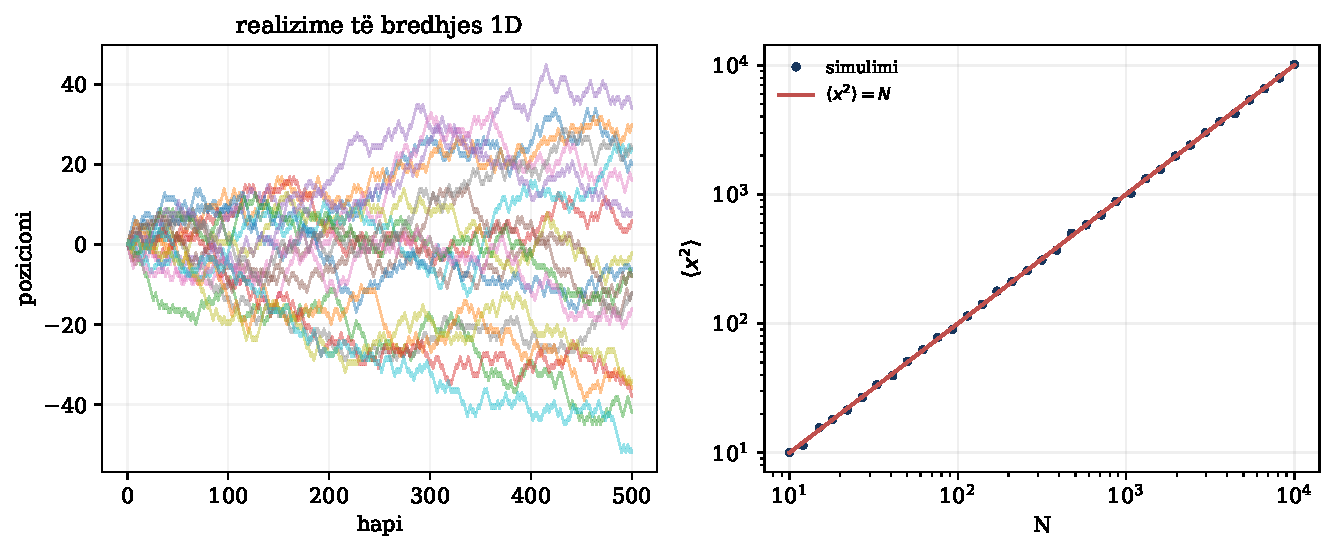
\includegraphics[width=.95\textwidth]{21_bredhja_e_rastit.pdf}
\caption{Realizime të bredhjes dhe rritja lineare e zhvendosjes katrore mesatare.}
\end{figure}

\section{Kufiri i vazhdueshëm dhe difuzioni}
Probabiliteti diskret plotëson ekuacionin master
\begin{equation}
 p_j^{n+1}=\tfrac12p_{j-1}^n+\tfrac12p_{j+1}^n.
\end{equation}
Zhvillimi Taylor dhe kufiri $\ell,\Delta t\to0$ me $\ell^2/(2\Delta t)=D$ japin
\begin{equation}
 \frac{\partial p}{\partial t}=D\frac{\partial^2p}{\partial x^2}.
\end{equation}
Për një grimcë fillimisht në origjinë,
\begin{equation}
 p(x,t)=\frac1{\sqrt{4\pi Dt}}\exp\left(-\frac{x^2}{4Dt}\right).
\end{equation}

\begin{figure}[ht]
\centering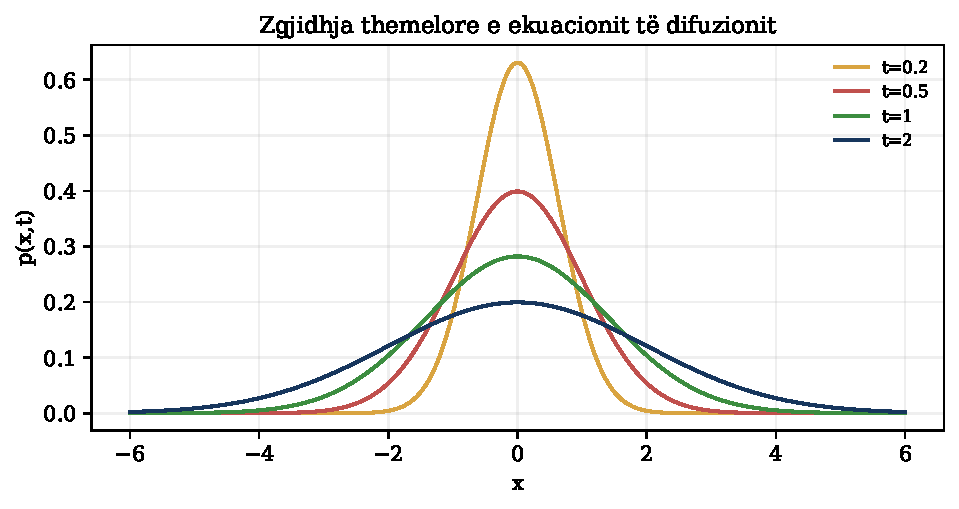
\includegraphics[width=.74\textwidth]{22_difuzioni_gaussian.pdf}
\caption{Profili i difuzionit zgjerohet, ndërsa normalizimi ruhet.}
\end{figure}

\section{Kufij, drift dhe kohë e parë kalimi}
Një kufi reflektues ruan grimcën; një kufi thithës e heq kur arrihet. Koha e parë e kalimit është koha kur trajektorja prek për herë të parë një objektiv. Me drift $v$,
\begin{equation}
 \frac{\partial p}{\partial t}=-v\frac{\partial p}{\partial x}+D\frac{\partial^2p}{\partial x^2}.
\end{equation}
Kjo lidh transportin determinist me luhatjet. Në mjedise heterogjene, hapi ose probabiliteti mund të varen nga pozicioni.

\section{Zinxhirët Markov}
Një proces diskret është Markov nëse e ardhmja, me kusht gjendjen e tanishme, nuk varet nga historia:
\begin{equation}
 P(X_{n+1}=j|X_n=i,X_{n-1},\ldots)=P_{ij}.
\end{equation}
Matrica $P$ ka elemente jo-negative dhe rreshta me shumë një. Shpërndarja evoluon si $\vect p_{n+1}=\vect p_nP$. Shpërndarja stacionare plotëson
\begin{equation}
 \vect\pi=\vect\pi P.
\end{equation}
Një zinxhir i fundmë, i pareduktueshëm dhe aperiodik ka shpërndarje stacionare unike dhe konvergon drejt saj.

\begin{figure}[ht]
\centering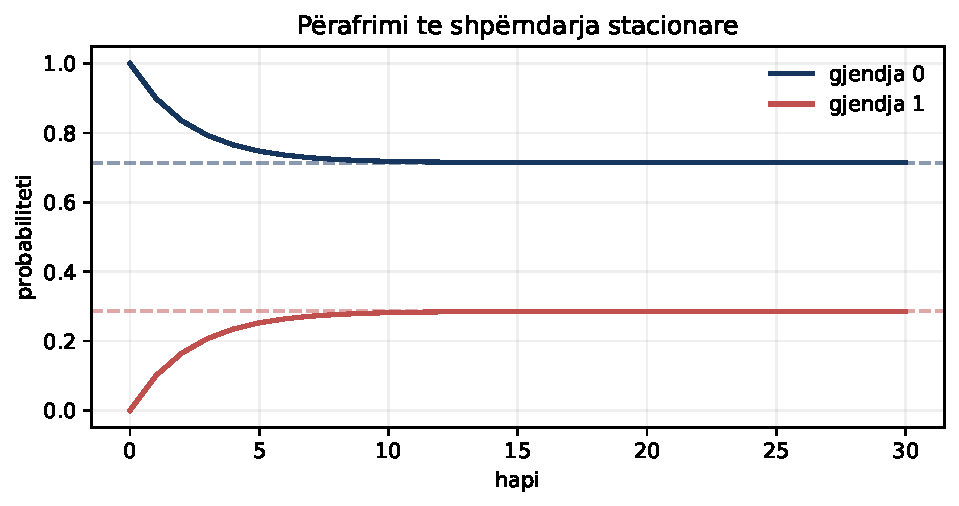
\includegraphics[width=.74\textwidth]{23_zinxhiri_markov.pdf}
\caption{Humbja graduale e kujtesës së gjendjes fillestare në një zinxhir me dy gjendje.}
\end{figure}

\section{Kthyeshmëria dhe balanca e detajuar}
Kushti
\begin{equation}
 \pi_iP_{ij}=\pi_jP_{ji}
\end{equation}
quhet balancë e detajuar. Ajo garanton stacionaritetin, por nuk është kusht i domosdoshëm. Interpretimi është ekuilibër i fluksit probabilitar ndërmjet çdo çifti gjendjesh.

\section{Korrelacioni dhe madhësia efektive}
Në një zinxhir, mostrat pasuese janë të korreluara. Për një observabël $A$,
\begin{equation}
 \rho_A(k)=\frac{\Cov(A_n,A_{n+k})}{\Var(A)},\qquad
 \tau_{\mathrm{int}}=\frac12+\sum_{k=1}^{\infty}\rho_A(k).
\end{equation}
Varianca e mesatares sillet afërsisht si
\begin{equation}
 \Var(\bar A)\approx\frac{2\tau_{\mathrm{int}}}{N}\Var(A),
\end{equation}
pra $N_{\mathrm{eff}}\approx N/(2\tau_{\mathrm{int}})$. Rritja e numrit të hapave nuk ndihmon shumë kur zinxhiri përzihet ngadalë.

\begin{lidhje}
Laboratori simulon bredhje 1D dhe 2D, mat $\avg{r^2}$, zbaton kufij thithës e reflektues dhe vlerëson kohën e korrelacionit të një zinxhiri të vogël.
\end{lidhje}

\section*{Pyetje kontrolli}
\begin{enumerate}
\item Si del ekuacioni i difuzionit nga ekuacioni master?
\item Çfarë dallimi ka stacionariteti nga pavarësia?
\item Pse $N$ hapa Markov nuk japin $N$ mostra të pavarura?
\end{enumerate}
\section{Algoritmet e bredhjes dhe të zinxhirit Markov}
\subsection{Bredhja dydimensionale}
\begin{lstlisting}[language=Python,caption={Shumë realizime të bredhjes në 2D.}]
def bredhje_2d(rng, n_realizime, n_hapa):
    drejtimi = rng.integers(0, 4, size=(n_realizime, n_hapa))
    dx = (drejtimi == 0) - (drejtimi == 1)
    dy = (drejtimi == 2) - (drejtimi == 3)
    x = np.c_[np.zeros(n_realizime), np.cumsum(dx, axis=1)]
    y = np.c_[np.zeros(n_realizime), np.cumsum(dy, axis=1)]
    return x, y

rng = np.random.default_rng(2026)
x, y = bredhje_2d(rng, 50_000, 2_000)
msd = np.mean(x*x + y*y, axis=0)
\end{lstlisting}
Përshtatja e $\avg{r^2}$ kundrejt kohës jep $4D$ në dy përmasa. Pikat e hershme dhe efektet e kufirit trajtohen veçmas.

\subsection{Kufiri thithës dhe koha e parë e kalimit}
\begin{lstlisting}[language=Python]
def koha_e_pare(x, prag):
    prekje = np.abs(x) >= prag
    ka = prekje.any(axis=1)
    t = np.full(len(x), np.nan)
    t[ka] = np.argmax(prekje[ka], axis=1)
    return t
\end{lstlisting}
Vlerat pa prekje janë të censuruara dhe nuk duhet të zëvendësohen me kohën maksimale pa e deklaruar.

\subsection{Evolucioni me matricë kalimi}
\begin{lstlisting}[language=Python,caption={Shpërndarja stacionare e një zinxhiri të fundmë.}]
P = np.array([[0.90, 0.10], [0.25, 0.75]])
p = np.array([1.0, 0.0])
for _ in range(100):
    p = p @ P
print(p, p @ P - p)

w, V = np.linalg.eig(P.T)
i = np.argmin(np.abs(w - 1.0))
pi = np.real(V[:, i]); pi /= pi.sum()
\end{lstlisting}

\subsection{Autokorrelacioni dhe $N_{\mathrm{eff}}$}
\begin{lstlisting}[language=Python,caption={Vlerësim fillestar i kohës së integruar të autokorrelacionit.}]
def autocorr(x, max_lag):
    x = np.asarray(x) - np.mean(x)
    c = np.correlate(x, x, mode="full")[len(x)-1:]
    c = c[:max_lag+1] / c[0]
    return c

rho = autocorr(observabli, 500)
pozitive = rho[1:][rho[1:] > 0]
tau_int = 0.5 + pozitive.sum()
N_eff = len(observabli)/(2*tau_int)
\end{lstlisting}
Prerja në vonesën e parë negative është rregull i thjeshtë, jo universal. Për analiza serioze përdoret dritare automatike ose bllokim.

\begin{lidhje}
Notebook-u duhet të paraqesë njëkohësisht trajektoret, $\avg{r^2}$, shpërndarjen e pozicionit dhe kohën e parë të kalimit. Secila mat një aspekt të ndryshëm të procesit.
\end{lidhje}

Për proceset e rastit dhe terminologjinë e statistikës janë konsultuar \cite{capollari,butka,tasho}; trajtimi i zinxhirëve Markov dhe autokorrelacionit mbështetet te \cite{robert,krauth}.

\subsection{Bredhja e rastit dhe kufiri i difuzionit}
Në një përmasë, hapi $\xi_n$ merr vlerat $\pm\ell$ me probabilitete të barabarta dhe
\begin{equation}
 X_N=\sum_{n=1}^{N}\xi_n.
\end{equation}
Pavarësia jep $\E[X_N]=0$ dhe $\Var(X_N)=N\ell^2$. Nëse një hap zgjat $\Delta t$, atëherë $t=N\Delta t$ dhe
\begin{equation}
 \E[X(t)^2]=\frac{\ell^2}{\Delta t}t=2Dt,
 \qquad D=\frac{\ell^2}{2\Delta t}.
\end{equation}
Për të marrë kufirin e vazhdueshëm mbahen $D$ dhe $t$ të fiksuara ndërsa $\ell,\Delta t\to0$. Shpërndarja e pozicionit i afrohet
\begin{equation}
 p(x,t)=\frac{1}{\sqrt{4\pi Dt}}\exp\left(-\frac{x^2}{4Dt}\right),
\end{equation}
që zgjidh $p_t=Dp_{xx}$. Ky është një shembull themelor ku një model mikroskopik stokastik çon në ekuacion makroskopik determinist.

Me drift, probabilitetet nuk janë të barabarta. Në kufirin e duhur shfaqet ekuacioni adveksion--difuzion
\begin{equation}
 p_t=-v p_x+Dp_{xx}.
\end{equation}
Kushtet thithëse përfaqësojnë largimin e grimcës; kushtet reflektuese ruajnë probabilitetin. Koha e parë e kalimit është ndryshore rasti dhe trajektoret që nuk e arrijnë kufirin brenda kohës së simulimit janë të censuruara, jo zero.

\subsection{Zinxhirët Markov dhe shpërndarja stacionare}
Për një zinxhir me hapësirë të fundme dhe matricë kalimi $P$, shpërndarja rresht evoluon si
\begin{equation}
 \vect\pi_{n+1}^T=\vect\pi_n^TP.
\end{equation}
Shpërndarja stacionare plotëson $\vect\pi^TP=\vect\pi^T$, $\pi_i\ge0$ dhe $\sum_i\pi_i=1$. Nëse zinxhiri është i pakthyeshëm dhe aperiodik, shpërndarja konvergon te stacionarja pavarësisht gjendjes fillestare. Shpejtësia lidhet me boshllëkun spektral ndërmjet vlerës vetjake $1$ dhe vlerës së dytë në modul.

Balanca e detajuar,
\begin{equation}
 \pi_iP_{ij}=\pi_jP_{ji},
\end{equation}
është kusht i mjaftueshëm për stacionaritet, sepse mbledhja sipas $i$ jep $(\vect\pi^TP)_j=\pi_j$. Ai nuk është kusht i domosdoshëm: mund të ketë rryma stacionare që nuk anulohen çift më çift.

\subsection{Autokorrelacioni dhe madhësia efektive}
Për një seri stacionare $A_n$, autokovarianca është
\begin{equation}
 C(k)=\E[(A_n-\mu)(A_{n+k}-\mu)],
 \qquad \rho(k)=C(k)/C(0).
\end{equation}
Varianca e mesatares për $N$ vëzhgime është
\begin{align}
 \Var(\overline A)&=\frac{1}{N^2}\sum_{i,j}\Cov(A_i,A_j)\\
 &\simeq\frac{C(0)}{N}\left[1+2\sum_{k=1}^{\infty}\rho(k)\right]
 =\frac{2\tau_{\mathrm{int}}C(0)}{N},
\end{align}
ku
\begin{equation}
 \tau_{\mathrm{int}}=\frac12+\sum_{k=1}^{\infty}\rho(k).
\end{equation}
Prandaj
\begin{equation}
 N_{\mathrm{eff}}=\frac{N}{2\tau_{\mathrm{int}}}.
\end{equation}
Formula $s/\sqrt N$ nënvlerëson gabimin kur mostrat janë të korreluara. Shuma e autokorrelacionit duhet prerë në një vonesë ku zhurma e vlerësimit nuk dominon; alternativa praktike janë mesataret në blloqe dhe shumë zinxhirë të pavarur.

\subsection{Koha e përzierjes dhe diagnostika}
Koha e përzierjes mat sa shpejt shpërndarja e zinxhirit harron gjendjen fillestare. Heqja e një numri fiks hapash pa diagnostikë nuk garanton termalizim. Vëzhgohen trajektoret, mesataret kumulative dhe krahasimi i zinxhirëve nga gjendje të ndryshme. Hollimi i zinxhirit zakonisht hedh informacion; ruajtja e të gjitha mostrave dhe përdorimi i $N_{\mathrm{eff}}$ është më transparent, përveç kufizimeve të ruajtjes ose kostos së vlerësimit.

\subsection{Përmbledhje dhe ushtrime}
Bredhja e rastit lidh fluktuacionet mikroskopike me difuzionin. Zinxhiri Markov shton varësinë kohore dhe kërkon korrigjimin e gabimit standard me autokorrelacionin.
\begin{enumerate}
\item Nxirrni $\E[r^2]=2dDt$ për bredhjen në $d$ përmasa.
\item Zgjidhni kohën mesatare të daljes nga një interval me kufij thithës.
\item Gjeni shpërndarjen stacionare dhe vlerat vetjake të një matrice kalimi $3\times3$.
\item Simuloni një zinxhir me dy gjendje dhe krahasoni $N_{\mathrm{eff}}$ teorik me atë të vlerësuar.
\item Tregoni me shembull se stacionariteti nuk nënkupton balancë të detajuar.
\end{enumerate}

\subsection{Koha mesatare e daljes}
Për bredhjen simetrike në nyjet $0,1,\ldots,L$ me kufij thithës, le të jetë $T_i$ numri mesatar i hapave deri në dalje kur nisemi nga $i$. Kushtëzimi ndaj hapit të parë jep
\begin{equation}
 T_i=1+\frac12T_{i-1}+\frac12T_{i+1},
 \qquad T_0=T_L=0.
\end{equation}
Riorganizimi jep diferencën e dytë
\begin{equation}
 T_{i+1}-2T_i+T_{i-1}=-2.
\end{equation}
Zgjidhja kuadratike që plotëson kufijtë është
\begin{equation}
 T_i=i(L-i).
\end{equation}
Në kufirin e difuzionit, koha mesatare $\tau(x)$ plotëson ekuacionin e prapëm
\begin{equation}
 D\tau''(x)=-1,qquad \tau(0)=\tau(a)=0,
\end{equation}
me zgjidhje $\tau(x)=x(a-x)/(2D)$. Kjo lidh drejtpërdrejt ekuacionin diskret me modelin e vazhdueshëm.

Nëse një kufi është reflektues, kushti bëhet derivat zero. Me drift, operatori i prapëm është $v\partial_x+D\partial_{xx}$. Kohët e para të kalimit janë të ndjeshme ndaj bishtave dhe kërkojnë shumë realizime; mesatarja vetëm mund të mos përshkruajë shpërndarjen.

\subsubsection{Spektri i matricës së kalimit}
Për një zinxhir të kthyeshëm, matrica e kalimit është vetë-adjunkte në prodhimin skalar të peshuar
\begin{equation}
 \langle f,g\rangle_\pi=\sum_i\pi_if_ig_i.
\end{equation}
Vlerat vetjake janë reale dhe plotësojnë $1=\lambda_1>\lambda_2\ge\cdots\ge-1$. Komponentët jo stacionarë shuhen si $\lambda_k^n$. Boshllëku spektral $1-\max_{k>1}|\lambda_k|$ kontrollon relaksimin më të ngadaltë.

Për një observabël që projektohet fort mbi modin e dytë, autokorrelacioni mund të sillet si $\rho(n)\simeq\lambda_2^n$. Atëherë
\begin{equation}
 \tau_{\mathrm{int}}\simeq\frac12+\frac{\lambda_2}{1-\lambda_2}
 =\frac{1+\lambda_2}{2(1-\lambda_2)}.
\end{equation}
Kjo tregon lidhjen ndërmjet përzierjes, boshllëkut spektral dhe gabimit të mesatares.

\subsubsection{Vlerësimi praktik i autokorrelacionit}
Vlerësuesi i autokovariancës në vonesën $k$ është
\begin{equation}
 \widehat C(k)=\frac{1}{N-k}\sum_{n=1}^{N-k}
 (A_n-\overline A)(A_{n+k}-\overline A).
\end{equation}
Për $k$ të madh mbeten pak çifte dhe vlerësuesi bëhet i zhurmshëm. Shuma naive deri në $N$ mund të luhatet fort. Përdoret një dritare vetëkonsistente: shuma ndalet kur $k$ është disa herë më i madh se $\widehat\tau_{\mathrm{int}}$, ose kur autokorrelacioni hyn në një rajon të pajtueshëm me zhurmën.

Metoda e blloqeve ndan serinë në blloqe me gjatësi $B$ dhe llogarit mesataren e çdo blloku. Kur $B\gg\tau$, mesataret e blloqeve janë afërsisht të pavarura. Gabimi i vlerësuar duhet të arrijë një pllajë me rritjen e $B$, para se numri i blloqeve të bëhet tepër i vogël.

\subsubsection{Ergodiciteti dhe kurthet}
Stacionariteti nuk mjafton nëse zinxhiri nuk mund të arrijë të gjithë mbështetjen. Një zinxhir i reduktueshëm mund të ketë disa shpërndarje stacionare dhe rezultati varet nga gjendja fillestare. Periodiciteti mund të shkaktojë alternim pa konvergjencë pikë për pikë, edhe kur mesataret kohore sillen më mirë.

Në hapësira me moda të ndara nga barriera, zinxhiri mund të jetë teorikisht ergodik, por praktikisht të mos kalojë barrierën gjatë simulimit. Trajektorja duket e qëndrueshme brenda një mode dhe jep pacaktueshmëri artificialisht të vogël. Nisja e shumë zinxhirëve, propozimet globale, temperimi ose metodat e grupimeve përdoren për të zbuluar dhe zbutur këtë problem.

\subsubsection{Renditja e faqeve dhe zinxhiri Markov}
Në renditjen e faqeve, kalimi ndjek një lidhje me probabilitet $\alpha$ dhe ``teleportohet'' me probabilitet $1-\alpha$. Termi i teleportimit e bën matricën pozitive, kështu që teorema Perron--Frobenius garanton një vektor stacionar unik pozitiv. Parametri $\alpha$ balancon respektimin e strukturës së lidhjeve me shpejtësinë e përzierjes.

Faqet pa dalje duhet të trajtohen: kolona përkatëse zëvendësohet me një shpërndarje probabilitare. Pa këtë hap, matrica nuk është stohastike dhe masa humbet. Ky shembull tregon se pastrimi i të dhënave është pjesë e modelit matematik, jo vetëm detaj programimi.


\chapter[Metropolis--Hastings dhe Monte Carlo në fizikën statistike]{Metropolis--Hastings dhe Monte Carlo\\në fizikën statistike}
\begin{qellime}
Studenti ndërton algoritmin Metropolis--Hastings; provon ruajtjen e shpërndarjes synuar; dallon termalizimin, përzierjen dhe autokorrelacionin; simulon modelin Ising dhe interpreton energjinë, magnetizimin, kapacitetin termik dhe tranzicionin fazor.
\end{qellime}

\section{Pse nevojitet MCMC}
Në fizikën statistike duam pritje sipas shpërndarjes Boltzmann,
\begin{equation}
 \pi(x)=\frac{e^{-\beta E(x)}}{Z},\qquad
 Z=\sum_xe^{-\beta E(x)}.
\end{equation}
Numri i gjendjeve rritet eksponencialisht dhe $Z$ është zakonisht i paarritshëm. Metodat Markov Chain Monte Carlo ndërtojnë një zinxhir me shpërndarje stacionare $\pi$ pa kërkuar konstanten e normalizimit.

\section{Algoritmi Metropolis--Hastings}
Nga gjendja $x$, propozohet $y\sim q(y|x)$ dhe pranohet me probabilitet
\begin{equation}
 \alpha(x,y)=\min\left[1,\frac{\pi(y)q(x|y)}{\pi(x)q(y|x)}\right].
\end{equation}
Nëse propozimi është simetrik,
\begin{equation}
 \alpha(x,y)=\min[1,e^{-\beta\Delta E}].
\end{equation}
Raporti anulon $Z$. Hapi i refuzuar nuk hidhet; gjendja e vjetër regjistrohet sërish. Kjo është e domosdoshme për shpërndarjen e saktë.

\begin{shembull}[Algoritmi Metropolis--Hastings]
Niset nga $x_0$. Për çdo hap propozohet $y\sim q(\cdot|x_n)$ dhe gjenerohet $u\sim\mathcal U(0,1)$. Llogaritet $a=\min\{1,\pi(y)q(x_n|y)/[\pi(x_n)q(y|x_n)]\}$. Nëse $u<a$, vendoset $x_{n+1}=y$; përndryshe vendoset $x_{n+1}=x_n$.
\end{shembull}

\section{Termalizimi dhe diagnostika}
Hapat e parë varen nga gjendja fillestare dhe hiqen si \emph{burn-in}. Gjatësia nuk zgjidhet me një numër universal; kontrollohen disa nisje, gjurmët, observablat dhe koha e autokorrelacionit. Hollimi i zinxhirit zakonisht hedh informacion dhe nuk zëvendëson vlerësimin e $N_{\mathrm{eff}}$.

Norma e pranimit nuk është qëllim në vetvete. Hapa shumë të vegjël pranohen shpesh, por lëvizin ngadalë; hapa shumë të mëdhenj refuzohen. Propozimi duhet të balancojë lëvizjen dhe pranimin. Për shpërndarje shumëmodale, zinxhiri mund të mbetet në një modë edhe kur gjurma duket e qëndrueshme.

\section{Modeli Ising dydimensional}
Në rrjet katror me spine $s_i=\pm1$,
\begin{equation}
 E=-J\sum_{\langle i,j\rangle}s_is_j-H\sum_is_i,
\qquad m=\frac1N\sum_is_i.
\end{equation}
Me kufij periodikë, çdo spin ka katër fqinjë. Për një kthim $s_i\to-s_i$,
\begin{equation}
 \Delta E=2s_i\left(J\sum_{j\in\mathrm{fqinj}}s_j+H\right).
\end{equation}
Në temperaturë të ulët, gjendjet e rreshtuara dominojnë; në temperaturë të lartë, entropia prodhon çrregullim.

\begin{figure}[ht]
\centering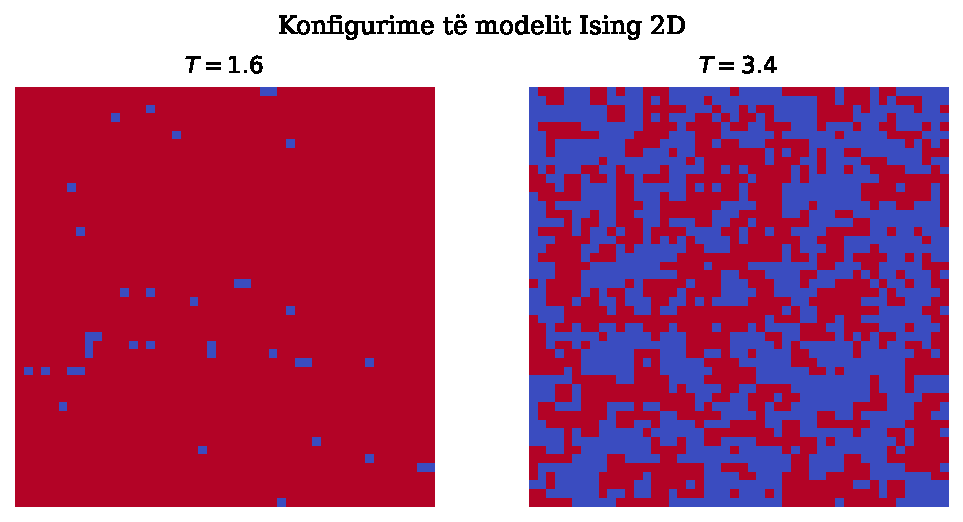
\includegraphics[width=.78\textwidth]{24_ising_konfigurime.pdf}
\caption{Formimi i domeneve nën temperaturën kritike dhe çrregullimi sipër saj.}
\end{figure}

\section{Observablat termodinamike}
Nga luhatjet merren
\begin{equation}
 C_V=\frac{\beta^2}{N}(\avg{E^2}-\avg E^2),
 \qquad
 \chi=\frac{\beta}{N}(\avg{M^2}-\avg M^2).
\end{equation}
Në sistem të fundmë, tranzicioni shfaqet si maksimum i gjerë, jo singularitet i vërtetë. Temperatura kritike e rrjetit katror pa fushë është
\begin{equation}
 \frac{k_BT_c}{J}=\frac{2}{\ln(1+\sqrt2)}\approx2.269.
\end{equation}

\begin{figure}[ht]
\centering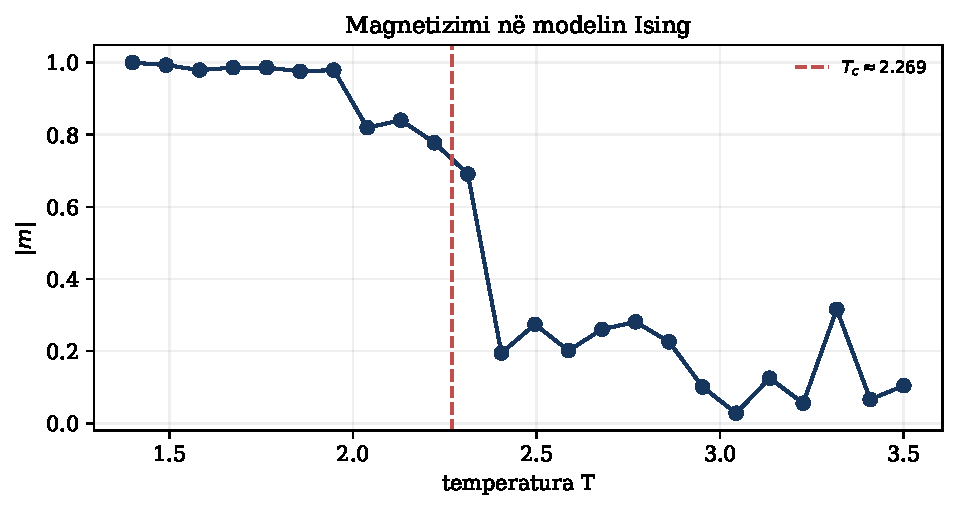
\includegraphics[width=.74\textwidth]{25_ising_magnetizimi.pdf}
\caption{Rënia e magnetizimit pranë zonës kritike në një simulim të fundmë.}
\end{figure}

\subsection{Ngadalësimi kritik dhe përmirësimet}
Pranë $T_c$, domenet ekzistojnë në shumë shkallë dhe përditësimi me një spin përzihet ngadalë. Koha e autokorrelacionit rritet me madhësinë e sistemit. Algoritmet e grupeve, si Wolff dhe Swendsen--Wang, ndryshojnë bashkë rajone të korreluara dhe ulin ngadalësimin kritik.

\subsection{Gabimet dhe analiza e të dhënave MCMC}
Mesatarja llogaritet pas termalizimit, por gabimi nuk merret duke trajtuar çdo hap si të pavarur. Përdoren autokorrelacioni i integruar, bllokimi ose batch means. Simulime të pavarura me fara të ndryshme ndihmojnë të zbulohet mos-përzierja.

\begin{kujdes}
Një konfigurim tërheqës vizualisht nuk është rezultat termodinamik. Përfundimet kërkojnë seri të termalizuara, madhësi efektive, prova me përmasa të ndryshme të rrjetit dhe observabla me gabime statistike.
\end{kujdes}

\subsection{Nga Ising te probleme të tjera}
I njëjti parim përdoret në mekanikën statistike, inferencën Bayesiane, modelet e materialeve dhe fushat në rrjet. Ndryshojnë energjia, hapësira e gjendjeve dhe propozimi; mbeten invarianca e shpërndarjes, ergodiciteti dhe analiza e korrelacionit.

\begin{lidhje}
Laboratori zbaton Ising 2D me Metropolis, verifikon $\Delta E$, mat normën e pranimit, termalizimin dhe autokorrelacionin, pastaj paraqet $|m|$, $C_V$ dhe $\chi$ kundrejt temperaturës.
\end{lidhje}

\section*{Pyetje kontrolli}
\begin{enumerate}
\item Pse konstanta e normalizimit anulohet në raportin Metropolis?
\item Pse hapat e refuzuar duhet të regjistrohen?
\item Çfarë është ngadalësimi kritik dhe si ndikon në gabimin statistik?
\item Pse një simulim me një madhësi rrjeti nuk mjafton për të vërtetuar tranzicion fazor?
\end{enumerate}
\section{Algoritmi Metropolis për modelin Ising}
\subsection{Energjia lokale dhe një sweep}
\begin{lstlisting}[language=Python,caption={Përditësimi Metropolis me një spin.}]
def delta_E(spin, i, j, J=1.0, H=0.0):
    L = spin.shape[0]
    fq = (spin[(i+1) % L, j] + spin[(i-1) % L, j]
          + spin[i, (j+1) % L] + spin[i, (j-1) % L])
    return 2.0*spin[i, j]*(J*fq + H)

def sweep_metropolis(spin, beta, rng, J=1.0, H=0.0):
    L = spin.shape[0]
    pranuar = 0
    for _ in range(L*L):
        i, j = rng.integers(0, L, size=2)
        dE = delta_E(spin, i, j, J, H)
        if dE <= 0.0 or rng.random() < np.exp(-beta*dE):
            spin[i, j] *= -1
            pranuar += 1
    return pranuar/(L*L)
\end{lstlisting}

\subsection{Matja e energjisë pa numërim të dyfishtë}
\begin{lstlisting}[language=Python]
def observablat(spin, J=1.0, H=0.0):
    djathtas = np.roll(spin, -1, axis=1)
    poshte = np.roll(spin, -1, axis=0)
    E = -J*np.sum(spin*(djathtas + poshte)) - H*np.sum(spin)
    M = np.sum(spin)
    return E, M
\end{lstlisting}
Numërohen vetëm lidhjet djathtas dhe poshtë, në mënyrë që çdo çift fqinjësh të hyjë një herë.

\subsection{Termalizimi dhe matjet}
\begin{lstlisting}[language=Python,caption={Struktura e një simulimi të plotë.}]
def simulo_ising(L, T, n_term, n_matje, hendek, seed):
    rng = np.random.default_rng(seed)
    spin = rng.choice([-1, 1], size=(L, L))
    beta = 1.0/T
    for _ in range(n_term):
        sweep_metropolis(spin, beta, rng)
    E, M = [], []
    for _ in range(n_matje):
        for _ in range(hendek):
            sweep_metropolis(spin, beta, rng)
        e, m = observablat(spin)
        E.append(e); M.append(m)
    return np.asarray(E), np.asarray(M)
\end{lstlisting}
Hendeku nuk garanton pavarësi. Autokorrelacioni matet dhe raportohet $N_{\mathrm{eff}}$.

\subsection{Observablat dhe gabimet}
\begin{lstlisting}[language=Python]
N = L*L
e = E/N; m = M/N
Cv = (np.mean(E**2) - np.mean(E)**2)/(N*T*T)
chi = (np.mean(M**2) - np.mean(M)**2)/(N*T)
m_abs = np.mean(np.abs(m))
\end{lstlisting}
Për gabimet përdoret bllokimi: seria ndahet në blloqe më të gjata se koha e korrelacionit dhe mesataret e blloqeve trajtohen si afërsisht të pavarura.

\subsection{Protokolli i studimit termik}
\begin{enumerate}
\item Ekzekutohen disa temperatura larg dhe pranë $T_c$.
\item Për çdo temperaturë kontrollohen termalizimi dhe pranimi.
\item Raportohen $\avg{|m|}$, $\avg e$, $C_V$, $\chi$ dhe gabimet.
\item Përsëritet për disa $L$ për të dalluar efektet e përmasës së fundme.
\item Krahasohen nisja e rregullt dhe e çrregullt pranë zonës kritike.
\end{enumerate}

\begin{kujdes}
Përdoren \emph{balancë e detajuar}, \emph{shpërndarje stacionare}, \emph{termalizim}, \emph{përzierje}, \emph{kohë autokorrelacioni} dhe \emph{ngadalësim kritik}. Këto terma përkufizohen para përdorimit dhe nuk zëvendësohen me anglicizma të panevojshëm.
\end{kujdes}

Termat e fizikës statistike janë harmonizuar me përdorimin universitar në shqip dhe me burimet probabilitare \cite{capollari,butka}; algoritmi dhe analiza MCMC mbështeten te burimet themelore \cite{metropolis,hastings,krauth,robert,walter}.

\subsection{Ndërtimi i Metropolis--Hastings nga balanca e detajuar}
Synohet shpërndarja $\pi(x)$, e njohur deri në një konstante normalizimi. Nga gjendja $x$ propozohet $y\sim q(y|x)$ dhe pranohet me probabilitet
\begin{equation}
 \alpha(x,y)=\min\left\{1,
 \frac{\pi(y)q(x|y)}{\pi(x)q(y|x)}\right\}.
\end{equation}
Për $x\ne y$, kerneli i kalimit është $T(x,y)=q(y|x)\alpha(x,y)$. Nëse raporti është më i vogël se një,
\begin{equation}
 \pi(x)T(x,y)=\pi(x)q(y|x)
 \frac{\pi(y)q(x|y)}{\pi(x)q(y|x)}
 =\pi(y)q(x|y),
\end{equation}
ndërsa kalimi i kundërt pranohet me probabilitet një. Rasti tjetër është simetrik; kështu vlen balanca e detajuar. Probabiliteti i refuzimit vendos masën e mbetur në $T(x,x)$ dhe siguron normalizimin.

Kur $q(y|x)=q(x|y)$, raporti i propozimit anulohet. Për shpërndarjen Boltzmann $\pi(x)\propto e^{-\beta E(x)}$ merret
\begin{equation}
 \alpha=\min\{1,e^{-\beta\Delta E}\}.
\end{equation}
Konstantja e ndarjes nuk llogaritet: ky është një nga avantazhet kryesore të MCMC.

\subsection{Zgjedhja e propozimit, pranimi dhe përzierja}
Një hap shumë i vogël pranohet shpesh, por lëviz ngadalë; një hap shumë i madh refuzohet shpesh. Norma e pranimit nuk është objektivi i vetëm. Duhet parë largësia e përshkuar, autokorrelacioni dhe $N_{\mathrm{eff}}$ për koston llogaritëse. Propozimi duhet të ruajë mbështetjen e synuar dhe ta bëjë zinxhirin të pakthyeshëm e aperiodik.

Termalizimi hiqet vetëm pas kontrollit të trajektoreve nga gjendje të shpërndara. Pastaj maten observablat në pjesën stacionare. Përfundimi shoqërohet me kohën e integruar të autokorrelacionit, madhësinë efektive dhe, kur është e mundur, krahasimin e shumë zinxhirëve.

\subsection{Modeli Ising dydimensional}
Në një rrjet katror me $N=L^2$ spine $s_i=\pm1$ dhe kufij periodikë,
\begin{equation}
 E=-J\sum_{\langle i,j\rangle}s_is_j-H\sum_i s_i,
 \qquad M=\sum_i s_i.
\end{equation}
Çdo lidhje numërohet një herë. Kur përmbyset spini $s_i$, vetëm lidhjet lokale ndryshojnë dhe
\begin{equation}
 \Delta E=2s_i\left(J\sum_{j\in\mathrm{fq}(i)}s_j+H\right).
\end{equation}
Ky rezultat shmang rillogaritjen e energjisë së gjithë rrjetit dhe ul koston e një prove nga $\Oh(N)$ në $\Oh(1)$. Një sweep përmban $N$ prova, pra kushton $\Oh(N)$.

Observablat termodinamike për spin janë
\begin{equation}
 e=\frac{\langle E\rangle}{N},\qquad
 m=\frac{\langle |M|\rangle}{N},
\end{equation}
\begin{equation}
 C_V=\frac{\beta^2}{N}\left(\langle E^2\rangle-\langle E\rangle^2\right),
 \qquad
 \chi=\frac{\beta}{N}\left(\langle M^2\rangle-\langle M\rangle^2\right).
\end{equation}
Përdorimi i $|M|$ në magnetizim shmang anulimin ndërmjet dy fazave të simetrisë në një rrjet të fundëm, por për susceptibilitetin duhet deklaruar qartë nëse përdoret $M$ apo $|M|$.

\subsection{Gabimet e matjeve të korreluara}
Mesatarja e energjisë nuk ka gabim $s_E/\sqrt{N_{\mathrm{matjeve}}}$ kur konfigurimet vijnë nga i njëjti zinxhir. Përdoret
\begin{equation}
 \operatorname{SE}(\overline E)=
 \sqrt{\frac{2\tau_{\mathrm{int},E}\Var(E)}{N_{\mathrm{matjeve}}}}.
\end{equation}
Për $C_V$ dhe $\chi$, që janë funksione jolineare të momenteve, bllokimi ose jackknife ruan korrelacionet dhe përhap pacaktueshmërinë. Madhësia e bllokut duhet të jetë dukshëm më e madhe se koha e autokorrelacionit; qëndrueshmëria e gabimit ndaj rritjes së bllokut është diagnostikë.

\subsection{Ngadalësimi kritik dhe madhësia e fundme}
Pranë temperaturës kritike, gjatësia e korrelacionit rritet dhe përditësimet lokale ndryshojnë vetëm ngadalë domenet e mëdha. Koha e autokorrelacionit rritet afërsisht si $\tau\sim L^z$. Ky ngadalësim kritik ul rëndë $N_{\mathrm{eff}}$. Algoritmet e grupimeve Wolff ose Swendsen--Wang përmbysin rajone të korreluara dhe mund ta zvogëlojnë këtë efekt, por Metropolis-i mbetet themeli pedagogjik për balancën e detajuar.

Për rrjet të fundëm nuk ka singularitet të vërtetë. Kulmet e $C_V$ dhe $\chi$ zhvendosen dhe mprehen me $L$. Prandaj një temperaturë kritike e vlerësuar nga një rrjet i vetëm është rezultat me efekt madhësie të fundme, jo kufiri termodinamik.

\begin{lstlisting}[language=Python,caption={Një sweep Metropolis për modelin Ising.}]
import numpy as np

def sweep_metropolis(spin, beta, rng, J=1.0, H=0.0):
    L = spin.shape[0]
    for _ in range(L * L):
        i = rng.integers(L); j = rng.integers(L)
        fqinjet = (spin[(i+1) % L, j] + spin[(i-1) % L, j]
                 + spin[i, (j+1) % L] + spin[i, (j-1) % L])
        delta_E = 2.0 * spin[i, j] * (J * fqinjet + H)
        if delta_E <= 0.0 or rng.random() < np.exp(-beta * delta_E):
            spin[i, j] *= -1
    return spin
\end{lstlisting}

\subsection{Protokolli i një studimi të riprodhueshëm}
Një studim termik duhet të deklarojë $L$, $J$, $H$, temperaturat, farat, gjendjet fillestare, numrin e sweeps të termalizimit, numrin e matjeve dhe mënyrën e vlerësimit të autokorrelacionit. Duhet provuar energjia lokale ndaj rillogaritjes së plotë në rrjete të vogla, të krahasohen kufijtë $T\to0$ dhe $T\to\infty$, dhe të kontrollohet simetria $M\leftrightarrow-M$ kur $H=0$.

\subsection{Përmbledhje dhe ushtrime}
Metropolis--Hastings ndërton një dinamikë artificiale me shpërndarje stacionare të zgjedhur. Koha Monte Carlo nuk është domosdoshmërisht kohë fizike; interpretimi termodinamik vjen nga shpërndarja e ekuilibrit.
\begin{enumerate}
\item Provoni balancën e detajuar për raportin e përgjithshëm Hastings.
\item Nxirrni $\Delta E$ për përmbysjen e një spini dhe kontrolloni numërimin e dyfishtë të lidhjeve.
\item Matni $\tau_{\mathrm{int}}$ të energjisë dhe magnetizimit në disa temperatura.
\item Krahasoni nisjen e renditur dhe të çrregullt për të përcaktuar termalizimin.
\item Kryeni studim me disa $L$ dhe diskutoni zhvendosjen e kulmit të susceptibilitetit.
\item Implementoni bllokimin ose jackknife për pacaktueshmërinë e kapacitetit termik.
\end{enumerate}

\subsection{Kufijtë analitikë të modelit Ising}
Në temperaturë zero dhe $H=0$, energjia minimizohet kur të gjitha spinet janë të njëjta. Në rrjetin katror çdo spin ka katër fqinjë, por çdo lidhje numërohet një herë; ka $2N$ lidhje. Prandaj energjia bazë është
\begin{equation}
 E_0=-2JN,qquad e_0=-2J.
\end{equation}
Magnetizimi për spin ka modul një. Këto janë teste të drejtpërdrejta për kodin në temperaturë të ulët.

Në temperaturë të pafundme, konfigurimet janë të barasvlershme dhe spinet janë të pavarura me mesatare zero. Atëherë $\langle E\rangle\to0$, $\langle M\rangle=0$ dhe
\begin{equation}
 \langle M^2\rangle=N.
\end{equation}
Prandaj $\langle M^2\rangle/N^2=1/N$. Një simulim me temperaturë shumë të lartë duhet t'i afrohet këtyre kufijve. Për rrjete shumë të vogla, të gjitha $2^N$ konfigurimet mund të enumerohen dhe të japin vlera të sakta të funksionit të ndarjes; ky është testi më i fortë i algoritmit dhe i observablave.

\subsubsection{Pranimi dhe bilanci energjetik lokal}
Në $H=0$, shuma e katër fqinjëve merr vlerat $-4,-2,0,2,4$. Për rrjedhojë, ndryshimi i energjisë kufizohet në bashkësinë
\begin{equation}
 \Delta E\in\{-8J,-4J,0,4J,8J\}.
\end{equation}
Faktorët $e^{-4\beta J}$ dhe $e^{-8\beta J}$ mund të parallogariten. Ky optimizim shmang eksponencialen në çdo provë dhe ruan saktësisht algoritmin.

Një matje e energjisë duhet të numërojë vetëm lidhjet djathtas dhe lart, ose të ndajë me dy shumën mbi të katër fqinjët. Gabimi i numërimit të dyfishtë ndryshon energjinë dhe temperaturën efektive. Testi lokal zgjedh një spin, llogarit energjinë e plotë para dhe pas përmbysjes dhe kontrollon barazinë me formulën e $\Delta E$ për shumë konfigurime të rastit.

\subsubsection{Kapaciteti termik, susceptibiliteti dhe cumulanti Binder}
Derivimi i pritjes kanonike jep
\begin{equation}
 \frac{\partial\langle E\rangle}{\partial\beta}
 =-\left(\langle E^2\rangle-\langle E\rangle^2\right).
\end{equation}
Me $\beta=1/(k_BT)$ merret formula e fluktuacioneve për $C_V$. Në mënyrë analoge, derivimi ndaj fushës jep susceptibilitetin nga fluktuacionet e magnetizimit. Këto marrëdhënie lidhin përgjigjen makroskopike me luhatjet mikroskopike.

Cumulanti Binder për magnetizimin është
\begin{equation}
 U_L=1-\frac{\langle M^4\rangle}{3\langle M^2\rangle^2}.
\end{equation}
Në fazën e çrregullt Gauss, $U_L\to0$; në një shpërndarje me dy maja të ngushta pranë $\pm M_0$, $U_L\to2/3$. Kurbat për madhësi të ndryshme rrjeti priten pranë temperaturës kritike, duke dhënë një vlerësim më robust se maksimumi i një observable të vetëm.

\subsubsection{Shkallëzimi me madhësinë e fundme}
Pranë pikës kritike, gjatësia e korrelacionit sillet si $\xi\sim|t|^{-\nu}$, ku $t=(T-T_c)/T_c$. Në rrjet të fundëm, rritja ndalet kur $\xi\sim L$. Kjo çon në forma shkallëzimi, për shembull
\begin{equation}
 m(T,L)=L^{-\beta_m/\nu}\mathcal M(tL^{1/\nu}),
\end{equation}
ku $\beta_m$ është eksponent kritik, jo inversi i temperaturës. Në $T_c$, grafiku log--log i $m$ ndaj $L$ ka pjerrësi $-\beta_m/\nu$.

Maksimumi i susceptibilitetit rritet afërsisht si $L^{\gamma/\nu}$ dhe temperatura e pseudokritike zhvendoset si $L^{-1/\nu}$. Një studim serioz përdor disa madhësi, interpolon observablat me pacaktueshmëri dhe kontrollon shembjen e të dhënave. Një kurbë e vetme magnetizimi nuk mjafton për të përcaktuar tranzicionin.

\subsubsection{Jackknife për madhësi jolineare}
Le të ndahen matjet në $B$ blloqe. Për çdo $b$ llogaritet statistiku $\theta_{(b)}$ duke hequr bllokun $b$. Mesatarja jackknife është $\overline\theta_J=B^{-1}\sum_b\theta_{(b)}$ dhe varianca vlerësohet me
\begin{equation}
 \widehat{\Var}_J(\theta)=\frac{B-1}{B}
 \sum_{b=1}^{B}(\theta_{(b)}-\overline\theta_J)^2.
\end{equation}
Kjo metodë përhap kovariancën ndërmjet $\langle E\rangle$ dhe $\langle E^2\rangle$ në $C_V$, ose ndërmjet momenteve në cumulantin Binder. Blloqet duhet të jenë më të gjata se autokorrelacioni; përndryshe pseudo-mostrat nuk janë afërsisht të pavarura.

\subsubsection{Krahasimi i algoritmeve}
Kostoja nuk matet vetëm me sweeps. Krahasimi përdor kohën e procesorit për një mostër efektivisht të pavarur,
\begin{equation}
 C_{\mathrm{eff}}\propto C_{\mathrm{sweep}}\,2\tau_{\mathrm{int}}.
\end{equation}
Metropolis-i lokal ka sweep të lirë, por $\tau$ të madh pranë kritikës. Algoritmi Wolff ndërton një grup spinesh të lidhura dhe e përmbys; kostoja për hap ndryshon, por autokorrelacioni kritik zvogëlohet fort. Krahasimi duhet bërë për të njëjtin observable dhe të njëjtën madhësi rrjeti.

Koha Monte Carlo e këtyre algoritmeve nuk është dinamika reale e magnetit, përveç rasteve kur rregullat e përditësimit janë zgjedhur si model kinetik. Për observablat e ekuilibrit mjafton shpërndarja stacionare; për koha relaksimi fizik nevojitet model dinamik me interpretim të veçantë.


\appendix
\chapter{Fjalorth, standarde të kodit dhe ura drejt notebook-eve}
Kjo shtojcë standardizon gjuhën e përdorur në leksione dhe në laborator. Qëllimi është që termi fizik, simboli matematik dhe emri në kod të tregojnë të njëjtin koncept. Kur dokumentacioni i një biblioteke përdor termin anglisht, ai jepet në kllapa vetëm në paraqitjen e parë.

\section{Fjalorth i termave kryesorë}
\small
\begin{longtable}{p{.25\textwidth}p{.22\textwidth}p{.45\textwidth}}
\toprule
Termi në shqip & Termi ndërkombëtar & Kuptimi në këtë tekst\\ \midrule
\endfirsthead
\toprule
Termi në shqip & Termi ndërkombëtar & Kuptimi në këtë tekst\\ \midrule
\endhead
algoritëm & algorithm & Varg i fundmë hapash që prodhon një rezultat nga hyrjet.\\
zbatim & implementation & Realizimi i algoritmit në një gjuhë programimi.\\
rrjetë & grid, mesh & Bashkësia diskrete e pikave në kohë ose hapësirë.\\
hap & step size & Largësia $h$, $\Delta t$ ose $\Delta x$ ndërmjet pikave të rrjetës.\\
gabim absolut & absolute error & $|\tilde x-x|$.\\
gabim relativ & relative error & $|\tilde x-x|/|x|$, kur emëruesi është i përshtatshëm.\\
gabim i përparmë & forward error & Gabimi në rezultatin e llogaritur.\\
gabim i prapëm & backward error & Perturbimi minimal i të dhënave që e bën rezultatin të saktë.\\
gabim i këputjes & truncation error & Gabimi nga zëvendësimi i një procesi të pafundëm me formulë të fundme.\\
gabim rrumbullakimi & round-off error & Gabimi nga paraqitja dhe veprimet me saktësi të fundme.\\
kushtëzim & conditioning & Ndjeshmëria e problemit ndaj perturbimeve të hyrjeve.\\
qëndrueshmëri & stability & Kontrolli i përhapjes së gabimeve nga algoritmi.\\
pajtueshmëri & consistency & Përafrimi i formulës diskrete me ekuacionin kur hapi shkon në zero.\\
konvergjencë & convergence & Përafrimi i zgjidhjes numerike me zgjidhjen e problemit.\\
mbetje & residual & Diferenca që mbetet kur përafrimi zëvendësohet në ekuacion.\\
tolerancë & tolerance & Prag numerik për ndalim ose pranim.\\
metodë e shtjelluar & explicit method & Hapi i ri llogaritet drejtpërdrejt nga vlerat e njohura.\\
metodë e pashtjelluar & implicit method & Hapi i ri gjendet duke zgjidhur një ekuacion.\\
problem i vlerës fillestare & initial-value problem & Kushti jepet në kohën fillestare.\\
problem i vlerave kufitare & boundary-value problem & Kushtet jepen në kufij të ndryshëm të domenit.\\
përshtatje & fitting & Përcaktimi i parametrave të modelit nga të dhënat.\\
mbetje e regresit & regression residual & $r_i=y_i-\hat y_i$.\\
rizgjedhje & resampling & Ndërtimi i mostrave të reja nga të dhënat ekzistuese.\\
ndryshore rasti & random variable & Funksion numerik mbi hapësirën e rezultateve.\\
mostër & sample & Bashkësi realizimesh të një ndryshoreje rasti.\\
kampionim & sampling & Procedura e gjenerimit ose përzgjedhjes së mostrave.\\
vlerësues & estimator & Rregull që i shoqëron mostrës një vlerë për parametrin.\\
vlerësim & estimate & Vlera konkrete e prodhuar nga vlerësuesi.\\
gabim standard & standard error & Devijimi standard i shpërndarjes së vlerësuesit.\\
interval besimi & confidence interval & Procedurë intervalore me mbulim të përcaktuar në përsëritje.\\
pacaktueshmëri & uncertainty & Diapazoni i arsyeshëm i vlerave për shkak të informacionit të kufizuar.\\
luhatje & fluctuation & Variacion fizik ose statistik i observablit.\\
gjenerator pseudorastësor & pseudorandom generator & Algoritëm determinist që prodhon varg me veti të kërkuara statistike.\\
farë & seed & Gjendje fillestare që identifikon një varg pseudorastësor.\\
kampionim i rëndësisë & importance sampling & Kampionim nga një propozim dhe korrigjim me pesha.\\
variabël kontrollues & control variate & Madhësi me pritje të njohur që ul variancën e vlerësuesit.\\
bredhje e rastit & random walk & Proces i ndërtuar nga hapa të rastit.\\
zinxhir Markov & Markov chain & Proces ku kalimi i ardhshëm varet nga gjendja e tanishme.\\
shpërndarje stacionare & stationary distribution & Shpërndarje që nuk ndryshon nën operatorin e kalimit.\\
balancë e detajuar & detailed balance & Barazi e flukseve probabilitare ndërmjet çifteve të gjendjeve.\\
përzierje & mixing & Humbja e varësisë nga gjendja fillestare.\\
termalizim & thermalization & Përafrimi i simulimit të fizikës statistike drejt ekuilibrit.\\
kohë autokorrelacioni & autocorrelation time & Shkalla e varësisë ndërmjet mostrave të zinxhirit.\\
madhësi efektive e mostrës & effective sample size & Numri i përafërt i mostrave të pavarura me të njëjtën saktësi.\\
ngadalësim kritik & critical slowing down & Rritja e kohës së korrelacionit pranë tranzicionit kritik.\\
observabël & observable & Madhësi e matshme e llogaritur nga gjendja e sistemit.\\
vleftësim & validation & Kontrolli i përshtatshmërisë së modelit ndaj dukurisë reale.\\
verifikim & verification & Kontrolli nëse ekuacionet e zgjedhura zgjidhen saktë.\\
riprodhueshmëri & reproducibility & Mundësia për të marrë të njëjtin rezultat me të njëjtat të dhëna dhe procedurë.\\
\bottomrule
\end{longtable}
\normalsize

\section{Emërtimi i madhësive në kod}
Emrat duhet të jenë të shkurtër, por jo të paqartë. Simbolet standarde mund të ruhen kur konteksti është i qartë: \texttt{dt}, \texttt{dx}, \texttt{beta}, \texttt{omega}. Për madhësi të përpunuara përdoren emra përshkrues: \texttt{gabimi\_relativ}, \texttt{energji\_totale}, \texttt{koha\_autokorrelacionit}. Njësia jepet në docstring ose në emër kur rreziku i ngatërrimit është i madh.

\begin{lstlisting}[language=Python,caption={Funksion me kontratë të qartë numerike.}]
def shpejtesia_terminale(masa_kg: float,
                         g_ms2: float,
                         koeficienti_kg_s: float) -> float:
    """Kthen shpejtesine terminale [m/s] per rezistence lineare."""
    if masa_kg <= 0 or koeficienti_kg_s <= 0:
        raise ValueError("Masa dhe koeficienti duhet te jene pozitivë.")
    return masa_kg * g_ms2 / koeficienti_kg_s
\end{lstlisting}

\section{Struktura standarde e çdo notebook-u}
Çdo notebook i kursit duhet të ketë të njëjtën skelet pedagogjik. Kjo lejon që studenti të përqendrohet te fizika dhe metoda, jo te gjetja e strukturës së raportit.

\begin{enumerate}
\item \textbf{Titulli dhe pyetja fizike.} Një fjali që mund të marrë përgjigje numerike.
\item \textbf{Rezultatet e të nxënit.} Tre deri pesë aftësi të verifikueshme.
\item \textbf{Modeli.} Ekuacionet, supozimet, njësitë dhe domeni i vlefshmërisë.
\item \textbf{Algoritmi.} Hapat, rendi, stabiliteti, kostoja dhe kriteri i ndalimit.
\item \textbf{Zbatimi.} Funksione të vogla, parametra të përqendruar dhe komente për arsyen, jo për sintaksën e dukshme.
\item \textbf{Verifikimi.} Rast analitik, ligj ruajtjeje, mbetje ose provë konvergjence.
\item \textbf{Eksperimenti.} Ndryshohet një faktor në çdo seri; ruhen të dhënat e papërpunuara.
\item \textbf{Analiza.} Figura me njësi, tabela, gabim numerik dhe pacaktueshmëri.
\item \textbf{Interpretimi.} Përgjigjja fizike dhe kufijtë e saj.
\item \textbf{Detyra.} Ndryshim modeli, metode ose të dhënash që kërkon arsyetim të ri.
\end{enumerate}

\section{Kontrollet minimale të cilësisë}
\begin{longtable}{p{.24\textwidth}p{.68\textwidth}}
\toprule
Kontrolli & Pyetjet që duhet të marrin përgjigje\\ \midrule
\endfirsthead
\toprule Kontrolli & Pyetjet që duhet të marrin përgjigje\\ \midrule\endhead
Fizika & A janë njësitë të pajtueshme? A respektohen kufijtë dhe shenjat? A ka ligj ruajtjeje?\\
Matematika & A ekziston dhe është unike zgjidhja? A është problemi i mirëkushtëzuar?\\
Algoritmi & Cili është rendi? Cili është kushti i stabilitetit? Sa kushton në kohë dhe memorie?\\
Kodi & A testohen hyrjet? A shmangen inverset e panevojshme? A është fara e kontrolluar?\\
Konvergjenca & A ndryshon rezultati siç pritet kur përgjysmohet hapi ose rritet $N$?\\
Statistika & A janë mostrat të pavarura? A raportohet gabimi standard ose $N_{\mathrm{eff}}$?\\
Figura & A kanë boshtet emra dhe njësi? A dallohen të dhënat nga modeli?\\
Raportimi & A përmenden supozimet, tolerancat, versionet dhe kufijtë e përfundimit?\\
\bottomrule
\end{longtable}

\section{Lidhja ndërmjet kapitujve dhe laboratorëve}
\begin{longtable}{p{.08\textwidth}p{.35\textwidth}p{.47\textwidth}}
\toprule
Nr. & Boshti i leksionit & Produkti minimal i notebook-ut\\ \midrule
\endfirsthead
\toprule Nr. & Boshti i leksionit & Produkti minimal i notebook-ut\\ \midrule\endhead
1 & Programimi shkencor & Funksione, figura me njësi, test fillestar dhe raport i shkurtër.\\
2 & Gabimet dhe kushtëzimi & Grafik gabimi--hap dhe sistem me $\kappa(A)$ të ndryshueshme.\\
3 & Rrënjët, sistemet, modet & Krahasim konvergjence dhe mode normale masë--sustë.\\
4 & Interpolimi dhe regresi & Ligji i Keplerit, mbetje dhe pacaktueshmëri parametrash.\\
5 & Derivatet dhe integralet & Perioda e lavjerrësit dhe studim konvergjence.\\
6 & Ekuacionet diferenciale & Rënie, lavjerrës dhe orbitë me kontrolle energjie.\\
7 & Valët & Puls, valë e qëndrueshme, CFL dhe reflektim nga plazma.\\
8 & Probabiliteti & Hedhje monedhe, interval besimi dhe CLT empirike.\\
9 & Kampionimi & Gjenerim shpërndarjesh dhe teste të CDF-së e korrelacionit.\\
10 & Integrimi Monte Carlo & Integral shumëpërmasor, $N^{-1/2}$ dhe zbritje me pacaktueshmëri.\\
11 & Bredhjet dhe Markov & Difuzion, kohë e parë kalimi dhe $N_{\mathrm{eff}}$.\\
12 & Metropolis dhe Ising & Termalizim, autokorrelacion, magnetizim dhe efekte të përmasës.\\
\bottomrule
\end{longtable}

\section{Parimi i kalimit nga notebook-u te paketa}
Në fillim funksionet shkruhen pranë shpjegimit. Kur përdoren në dy ose më shumë notebook-e, ato zhvendosen në modul. Paketa përfundimtare duhet të ketë ndarje ndërmjet modelit, algoritmeve, analizës dhe paraqitjes. Testet ruhen veçmas dhe ekzekutohen pa hapur notebook-un.

\begin{lstlisting}[caption={Struktura e rekomanduar e paketës së studentit.}]
projekti/
|-- pyproject.toml
|-- README.md
|-- src/simulim_fizik/
|   |-- modele.py
|   |-- algoritme.py
|   |-- statistike.py
|   `-- vizualizim.py
|-- notebooks/
|   |-- 01_verifikimi.ipynb
|   `-- 02_eksperimenti.ipynb
|-- tests/
|   |-- test_modele.py
|   `-- test_algoritme.py
`-- results/
\end{lstlisting}

Kjo strukturë ruan parimin e kursit pararendës: notebook-u për kuptim dhe komunikim; paketa për ripërdorim, testim dhe zgjerim.

\section{Udhëzues i burimeve shkencore në shqip}
Literatura universitare në shqip përdoret në këtë tekst për tri qëllime: për terminologjinë, për rendin didaktik të analizës numerike dhe për shembujt që janë familjarë në programet shqiptare. Ajo plotësohet me literaturë ndërkombëtare kur kërkohen algoritme moderne, analiza të hollësishme të qëndrueshmërisë ose metoda Monte Carlo të avancuara.

\subsection{Analiza numerike me MATLAB}
Teksti i L. Hanellit dhe F. Osmanit \cite{hanelli} është burim qendror për trajtimin në shqip të gabimeve, ekuacioneve jolineare, sistemeve lineare, interpolimit, kuadraturës, ekuacioneve diferenciale dhe problemeve të vlerave vetjake. Në këto leksione ruhet ndarja e qartë ndërmjet problemit matematik, metodës dhe zbatimit, por shembujt e kodit janë përditësuar kryesisht në Python dhe lidhen me eksperimente fizike.

\subsection{Metoda të Analizës Numerike}
Teksti i F. Hoxhës \cite{hoxha} përdoret për përkufizimet, rendin e temave dhe emërtimet tradicionale shqip. Veçanërisht të dobishme janë dallimet ndërmjet gabimit, kushtëzimit, qëndrueshmërisë dhe konvergjencës. Në leksione këto koncepte shoqërohen me eksperimente kompjuterike, sepse studenti duhet t'i shohë si sjellje të matshme dhe jo vetëm si përkufizime.

\subsection{Leksionet e Universitetit Politeknik të Tiranës}
Materialet e R. Datjës \cite{datja} japin një urë të vlefshme ndërmjet analizës numerike, MATLAB-it dhe programeve inxhinierike. Ato janë përdorur për të kontrolluar terminologjinë e metodave të rrënjëve, interpolimit, kuadraturës dhe vlerave vetjake. Në këtë tekst ruhet lidhja me MATLAB/Octave, edhe kur snippet-i kryesor jepet në Python.

\subsection{Ekuacionet diferenciale dhe qëndrueshmëria}
Disertacioni dhe punimet e E. Dishmemës \cite{dishmema,dishmemaArticle} përmbajnë një trajtim të gjerë në shqip të metodave me një hap, gabimit lokal e global, pajtueshmërisë, konvergjencës dhe qëndrueshmërisë. Ky burim ka ndihmuar veçanërisht në përdorimin e termave \emph{metodë e shtjelluar} dhe \emph{metodë e pashtjelluar}. Leksionet tona fokusohen te ekuacionet e zakonshme pa vonesë, por parimet numerike janë të përbashkëta.

\subsection{Problemet kufitare dhe ekuacionet me derivate të pjesshme}
Puna e A. Naços \cite{naco} dhe materialet shqiptare të analizës numerike shërbejnë si pikë reference për problemet kufitare. Për valët, diferencat e fundme dhe kushtin CFL, këto burime plotësohen me tekstet e fizikës llogaritëse, sepse interpretimi fizik i dispersimit dhe reflektimit është po aq i rëndësishëm sa skema numerike.

\subsection{Probabiliteti, rizgjedhja dhe analiza e të dhënave}
Materialet e probabilitetit dhe statistikës \cite{capollari}, si edhe disertacionet mbi bootstrap-in dhe vlerat e humbura \cite{butka,tasho}, ndihmojnë në standardizimin e termave \emph{mostër}, \emph{vlerësues}, \emph{rizgjedhje}, \emph{gabim standard} dhe \emph{interval besimi}. Këto koncepte janë themelore për Monte Carlo-n, edhe kur objektivi përfundimtar është një integral ose një observabël termodinamik.

\subsection{Monte Carlo dhe fizika statistike}
Burimet e plota në shqip për MCMC dhe modelin Ising janë më të pakta. Për këtë arsye, terminologjia probabilitare lidhet me burimet shqiptare, ndërsa hollësitë algoritmike mbështeten te Metropolis et al., Hastings, Krauth dhe Robert--Casella \cite{metropolis,hastings,krauth,robert}. Ky kombinim shmang dy rreziqe: përkthimin mekanik të termave dhe thjeshtimin e tepërt të teorisë.

\section{Rruga e rekomanduar e leximit}
\begin{longtable}{p{.22\textwidth}p{.33\textwidth}p{.37\textwidth}}
\toprule
Nevoja e studentit & Kapitujt e këtij teksti & Burimet plotësuese\\ \midrule
\endfirsthead
\toprule Nevoja e studentit & Kapitujt e këtij teksti & Burimet plotësuese\\ \midrule\endhead
Bazat e gabimit dhe algoritmit & 1--2 & Hanelli--Osmani; Hoxha; Higham\\
Rrënjë dhe sisteme & 3 & Hanelli--Osmani; Datja; Burden--Faires\\
Vlera vetjake dhe mode & 3 & Datja; Newman; Landau et al.\\
Interpolim dhe përshtatje & 4 & Hanelli--Osmani; Hoxha; Press et al.\\
Derivim dhe kuadraturë & 5 & Hoxha; Datja; Newman\\
Ekuacione diferenciale & 6 & Dishmema; Hanelli--Osmani; Giordano--Nakanishi\\
Valë dhe diferenca të fundme & 7 & Naço; Giordano--Nakanishi; Landau et al.\\
Probabilitet dhe pacaktueshmëri & 8 & Çapollari et al.; Butka; Tasho Milo\\
Gjeneratorë dhe kampionim & 9 & Press et al.; Robert--Casella\\
Integrim Monte Carlo & 10 & Newman; Press et al.; Robert--Casella\\
Bredhje dhe Markov & 11 & Newman; Krauth; Robert--Casella\\
Metropolis dhe Ising & 12 & Metropolis et al.; Hastings; Krauth\\
\bottomrule
\end{longtable}

\section{Parime për citimin në notebook}
Kur një formulë, algoritëm ose grup të dhënash merret nga një burim, notebook-u duhet të japë autorin, titullin dhe vendin e saktë ku është përdorur. Dokumentacioni i NumPy, SciPy ose MATLAB citohet për sjelljen e funksionit të gatshëm; ai nuk zëvendëson burimin shkencor të metodës. Për figurat e prodhuara nga kodi i studentit shënohet ``llogaritje e autorit'' dhe ruhen skripti, parametrat dhe të dhënat që e gjeneruan.

Një listë e gjatë referencash nuk garanton cilësi. Çdo citim duhet të ketë rol të qartë: përkufizim, metodë, të dhëna, krahasim ose interpretim. Burimet në shqip ndihmojnë terminologjinë dhe vazhdimësinë akademike; burimet ndërkombëtare sigurojnë mbulimin e zhvillimeve dhe standardeve të fushës.


\backmatter
\chapter*{Përfundime}
Metodat numerike dhe Monte Carlo nuk janë vetëm teknika llogaritëse. Ato janë mënyra për të ndërtuar argumente shkencore kur zgjidhja analitike mungon, të dhënat kanë pacaktueshmëri ose hapësira e gjendjeve është shumë e madhe. Një simulim bindës bashkon modelin fizik, analizën e gabimit, kontrollin e kodit, eksperimentin numerik dhe interpretimin e matur.

\begin{thebibliography}{99}
\bibitem{hanelli} L. Hanelli dhe F. Osmani, \emph{Analiza numerike me MATLAB}, Pegi, Tiranë, 2013.
\bibitem{hoxha} F. Hoxha, \emph{Metoda të Analizës Numerike}, Tiranë, 2008.
\bibitem{datja} R. Datja, \emph{Analizë Numerike: leksione dhe seminare të shkruara për Inxhinieri Elektronike dhe Mekatronikë}, Universiteti Politeknik i Tiranës, 2022--2023.
\bibitem{dishmema} E. Dishmema, \emph{Metoda numerike për ekuacionet diferenciale me vonesa}, disertacion, Fakulteti i Shkencave të Natyrës, Universiteti i Tiranës, 2020.
\bibitem{dishmemaArticle} E. Dishmema et al., ``Krahasim i strategjive numerike për problemin e vlerës fillestare të ekuacioneve diferenciale të zakonshme dhe me vonesa'', \emph{Buletini i Shkencave të Natyrës}, Universiteti i Tiranës.
\bibitem{naco} A. Naço, \emph{Analizë krahasuese e metodave për zgjidhjen e problemit kufitar}, punim në Analizë Numerike, Universiteti Politeknik i Tiranës.
\bibitem{butka} A. Butka, \emph{Metoda bootstrap tek modelet e serive kohore, në veçanti tek modelet ARFIMA}, disertacion, Fakulteti i Shkencave të Natyrës, Universiteti i Tiranës.
\bibitem{tasho} E. Tasho Milo, \emph{Vlerat e humbura me metodat e rizgjedhjes}, disertacion, Programi Metodat Probabilitare, Statistike dhe Metodat e Analizës Numerike, Universiteti i Tiranës, 2019.
\bibitem{capollari} Gj. Çapollari dhe bashkautorë, \emph{Ushtrime probabiliteti dhe statistike}, material universitar, Tiranë, 2007.
\bibitem{zeqiri2020} A. Zeqiri et al., punim mbi algjebrën lineare numerike dhe metodat iterative, \emph{Buletini i Shkencave të Natyrës}, Universiteti i Tiranës, 29, 2020.
\bibitem{hyka} N. Hyka, materiale mësimore dhe trajnuese mbi metodat Monte Carlo dhe analizën e të dhënave, Universiteti i Mjekësisë, Tiranë.
\bibitem{newman} M. Newman, \emph{Computational Physics}, CreateSpace, 2012.
\bibitem{giordano} N. J. Giordano dhe H. Nakanishi, \emph{Computational Physics}, Pearson, 2005.
\bibitem{press} W. H. Press et al., \emph{Numerical Recipes}, 3rd ed., Cambridge University Press, 2007.
\bibitem{burden} R. L. Burden dhe J. D. Faires, \emph{Numerical Analysis}, 9th ed., Brooks/Cole, 2011.
\bibitem{higham} N. J. Higham, \emph{Accuracy and Stability of Numerical Algorithms}, 2nd ed., SIAM, 2002.
\bibitem{landau} R. H. Landau, M. J. Páez dhe C. C. Bordeianu, \emph{Computational Physics}, 3rd ed., Wiley-VCH, 2015.
\bibitem{krauth} W. Krauth, \emph{Statistical Mechanics: Algorithms and Computations}, Oxford University Press, 2006.
\bibitem{robert} C. P. Robert dhe G. Casella, \emph{Monte Carlo Statistical Methods}, 2nd ed., Springer, 2004.
\bibitem{metropolis} N. Metropolis et al., ``Equation of State Calculations by Fast Computing Machines'', \emph{J. Chem. Phys.} 21, 1087--1092, 1953.
\bibitem{hastings} W. K. Hastings, ``Monte Carlo Sampling Methods Using Markov Chains and Their Applications'', \emph{Biometrika} 57, 97--109, 1970.
\bibitem{walter} J.-C. Walter dhe G. T. Barkema, ``An Introduction to Monte Carlo Methods'', arXiv:1404.0209, 2014.
\end{thebibliography}
\end{document}
